\documentclass[twoside]{book}

% Packages required by doxygen
\usepackage{fixltx2e}
\usepackage{calc}
\usepackage{doxygen}
\usepackage[export]{adjustbox} % also loads graphicx
\usepackage{graphicx}
\usepackage[utf8]{inputenc}
\usepackage{makeidx}
\usepackage{multicol}
\usepackage{multirow}
\PassOptionsToPackage{warn}{textcomp}
\usepackage{textcomp}
\usepackage[nointegrals]{wasysym}
\usepackage[table]{xcolor}

% Font selection
\usepackage[T1]{fontenc}
\usepackage[scaled=.90]{helvet}
\usepackage{courier}
\usepackage{amssymb}
\usepackage{sectsty}
\renewcommand{\familydefault}{\sfdefault}
\allsectionsfont{%
  \fontseries{bc}\selectfont%
  \color{darkgray}%
}
\renewcommand{\DoxyLabelFont}{%
  \fontseries{bc}\selectfont%
  \color{darkgray}%
}
\newcommand{\+}{\discretionary{\mbox{\scriptsize$\hookleftarrow$}}{}{}}

% Page & text layout
\usepackage{geometry}
\geometry{%
  a4paper,%
  top=2.5cm,%
  bottom=2.5cm,%
  left=2.5cm,%
  right=2.5cm%
}
\tolerance=750
\hfuzz=15pt
\hbadness=750
\setlength{\emergencystretch}{15pt}
\setlength{\parindent}{0cm}
\setlength{\parskip}{3ex plus 2ex minus 2ex}
\makeatletter
\renewcommand{\paragraph}{%
  \@startsection{paragraph}{4}{0ex}{-1.0ex}{1.0ex}{%
    \normalfont\normalsize\bfseries\SS@parafont%
  }%
}
\renewcommand{\subparagraph}{%
  \@startsection{subparagraph}{5}{0ex}{-1.0ex}{1.0ex}{%
    \normalfont\normalsize\bfseries\SS@subparafont%
  }%
}
\makeatother

% Headers & footers
\usepackage{fancyhdr}
\pagestyle{fancyplain}
\fancyhead[LE]{\fancyplain{}{\bfseries\thepage}}
\fancyhead[CE]{\fancyplain{}{}}
\fancyhead[RE]{\fancyplain{}{\bfseries\leftmark}}
\fancyhead[LO]{\fancyplain{}{\bfseries\rightmark}}
\fancyhead[CO]{\fancyplain{}{}}
\fancyhead[RO]{\fancyplain{}{\bfseries\thepage}}
\fancyfoot[LE]{\fancyplain{}{}}
\fancyfoot[CE]{\fancyplain{}{}}
\fancyfoot[RE]{\fancyplain{}{\bfseries\scriptsize Generated by Doxygen }}
\fancyfoot[LO]{\fancyplain{}{\bfseries\scriptsize Generated by Doxygen }}
\fancyfoot[CO]{\fancyplain{}{}}
\fancyfoot[RO]{\fancyplain{}{}}
\renewcommand{\footrulewidth}{0.4pt}
\renewcommand{\chaptermark}[1]{%
  \markboth{#1}{}%
}
\renewcommand{\sectionmark}[1]{%
  \markright{\thesection\ #1}%
}

% Indices & bibliography
\usepackage{natbib}
\usepackage[titles]{tocloft}
\setcounter{tocdepth}{3}
\setcounter{secnumdepth}{5}
\makeindex

% Hyperlinks (required, but should be loaded last)
\usepackage{ifpdf}
\ifpdf
  \usepackage[pdftex,pagebackref=true]{hyperref}
\else
  \usepackage[ps2pdf,pagebackref=true]{hyperref}
\fi
\hypersetup{%
  colorlinks=true,%
  linkcolor=blue,%
  citecolor=blue,%
  unicode%
}

% Custom commands
\newcommand{\clearemptydoublepage}{%
  \newpage{\pagestyle{empty}\cleardoublepage}%
}

\usepackage{caption}
\captionsetup{labelsep=space,justification=centering,font={bf},singlelinecheck=off,skip=4pt,position=top}

%===== C O N T E N T S =====

\begin{document}

% Titlepage & ToC
\hypersetup{pageanchor=false,
             bookmarksnumbered=true,
             pdfencoding=unicode
            }
\pagenumbering{alph}
\begin{titlepage}
\vspace*{7cm}
\begin{center}%
{\Large Central\+Taxis }\\
\vspace*{1cm}
{\large Generated by Doxygen 1.8.12}\\
\end{center}
\end{titlepage}
\clearemptydoublepage
\pagenumbering{roman}
\tableofcontents
\clearemptydoublepage
\pagenumbering{arabic}
\hypersetup{pageanchor=true}

%--- Begin generated contents ---
\chapter{Hierarchical Index}
\section{Class Hierarchy}
This inheritance list is sorted roughly, but not completely, alphabetically\+:\begin{DoxyCompactList}
\item \contentsline{section}{Central\+Taxis}{\pageref{classCentralTaxis}}{}
\item \contentsline{section}{Customer}{\pageref{classCustomer}}{}
\begin{DoxyCompactList}
\item \contentsline{section}{Company\+Customer}{\pageref{classCompanyCustomer}}{}
\item \contentsline{section}{Private\+Customer}{\pageref{classPrivateCustomer}}{}
\end{DoxyCompactList}
\item \contentsline{section}{Date}{\pageref{classDate}}{}
\item \contentsline{section}{Invalid\+Distance\+Exception}{\pageref{classInvalidDistanceException}}{}
\item \contentsline{section}{Invalid\+Expected\+Time\+Exception}{\pageref{classInvalidExpectedTimeException}}{}
\item \contentsline{section}{Invalid\+Nif\+Exception}{\pageref{classInvalidNifException}}{}
\item \contentsline{section}{Invalid\+Phone\+Number\+Exception}{\pageref{classInvalidPhoneNumberException}}{}
\item \contentsline{section}{Route}{\pageref{classRoute}}{}
\item \contentsline{section}{Service}{\pageref{classService}}{}
\item \contentsline{section}{Voucher}{\pageref{classVoucher}}{}
\end{DoxyCompactList}

\chapter{Class Index}
\section{Class List}
Here are the classes, structs, unions and interfaces with brief descriptions\+:\begin{DoxyCompactList}
\item\contentsline{section}{\hyperlink{classCentralTaxis}{Central\+Taxis} }{\pageref{classCentralTaxis}}{}
\item\contentsline{section}{\hyperlink{classCompanyCustomer}{Company\+Customer} }{\pageref{classCompanyCustomer}}{}
\item\contentsline{section}{\hyperlink{classCustomer}{Customer} }{\pageref{classCustomer}}{}
\item\contentsline{section}{\hyperlink{classDate}{Date} }{\pageref{classDate}}{}
\item\contentsline{section}{\hyperlink{classInvalidDistanceException}{Invalid\+Distance\+Exception} }{\pageref{classInvalidDistanceException}}{}
\item\contentsline{section}{\hyperlink{classInvalidExpectedTimeException}{Invalid\+Expected\+Time\+Exception} }{\pageref{classInvalidExpectedTimeException}}{}
\item\contentsline{section}{\hyperlink{classInvalidNifException}{Invalid\+Nif\+Exception} }{\pageref{classInvalidNifException}}{}
\item\contentsline{section}{\hyperlink{classInvalidPhoneNumberException}{Invalid\+Phone\+Number\+Exception} }{\pageref{classInvalidPhoneNumberException}}{}
\item\contentsline{section}{\hyperlink{classPrivateCustomer}{Private\+Customer} }{\pageref{classPrivateCustomer}}{}
\item\contentsline{section}{\hyperlink{classRoute}{Route} }{\pageref{classRoute}}{}
\item\contentsline{section}{\hyperlink{classService}{Service} }{\pageref{classService}}{}
\item\contentsline{section}{\hyperlink{classVoucher}{Voucher} }{\pageref{classVoucher}}{}
\end{DoxyCompactList}

\chapter{File Index}
\section{File List}
Here is a list of all files with brief descriptions\+:\begin{DoxyCompactList}
\item\contentsline{section}{src/\hyperlink{CentralTaxis_8cpp}{Central\+Taxis.\+cpp} }{\pageref{CentralTaxis_8cpp}}{}
\item\contentsline{section}{src/\hyperlink{CentralTaxis_8h}{Central\+Taxis.\+h} }{\pageref{CentralTaxis_8h}}{}
\item\contentsline{section}{src/\hyperlink{CompanyCustomer_8cpp}{Company\+Customer.\+cpp} }{\pageref{CompanyCustomer_8cpp}}{}
\item\contentsline{section}{src/\hyperlink{CompanyCustomer_8h}{Company\+Customer.\+h} }{\pageref{CompanyCustomer_8h}}{}
\item\contentsline{section}{src/\hyperlink{Customer_8cpp}{Customer.\+cpp} }{\pageref{Customer_8cpp}}{}
\item\contentsline{section}{src/\hyperlink{Customer_8h}{Customer.\+h} }{\pageref{Customer_8h}}{}
\item\contentsline{section}{src/\hyperlink{Date_8cpp}{Date.\+cpp} }{\pageref{Date_8cpp}}{}
\item\contentsline{section}{src/\hyperlink{Date_8h}{Date.\+h} }{\pageref{Date_8h}}{}
\item\contentsline{section}{src/\hyperlink{main_8cpp}{main.\+cpp} }{\pageref{main_8cpp}}{}
\item\contentsline{section}{src/\hyperlink{Menu_8cpp}{Menu.\+cpp} }{\pageref{Menu_8cpp}}{}
\item\contentsline{section}{src/\hyperlink{Menu_8h}{Menu.\+h} }{\pageref{Menu_8h}}{}
\item\contentsline{section}{src/\hyperlink{PrivateCustomer_8cpp}{Private\+Customer.\+cpp} }{\pageref{PrivateCustomer_8cpp}}{}
\item\contentsline{section}{src/\hyperlink{PrivateCustomer_8h}{Private\+Customer.\+h} }{\pageref{PrivateCustomer_8h}}{}
\item\contentsline{section}{src/\hyperlink{Route_8cpp}{Route.\+cpp} }{\pageref{Route_8cpp}}{}
\item\contentsline{section}{src/\hyperlink{Route_8h}{Route.\+h} }{\pageref{Route_8h}}{}
\item\contentsline{section}{src/\hyperlink{Service_8cpp}{Service.\+cpp} }{\pageref{Service_8cpp}}{}
\item\contentsline{section}{src/\hyperlink{Service_8h}{Service.\+h} }{\pageref{Service_8h}}{}
\item\contentsline{section}{src/\hyperlink{utilities_8h}{utilities.\+h} }{\pageref{utilities_8h}}{}
\item\contentsline{section}{src/\hyperlink{Voucher_8cpp}{Voucher.\+cpp} }{\pageref{Voucher_8cpp}}{}
\item\contentsline{section}{src/\hyperlink{Voucher_8h}{Voucher.\+h} }{\pageref{Voucher_8h}}{}
\end{DoxyCompactList}

\chapter{Class Documentation}
\hypertarget{classCentralTaxis}{}\section{Central\+Taxis Class Reference}
\label{classCentralTaxis}\index{Central\+Taxis@{Central\+Taxis}}


{\ttfamily \#include $<$Central\+Taxis.\+h$>$}

\subsection*{Public Member Functions}
\begin{DoxyCompactItemize}
\item 
\hyperlink{classCentralTaxis_aca0cca3a2df44dadf8bfcb71b3636739}{Central\+Taxis} (string \hyperlink{classCentralTaxis_ab651d92a544bb7910586183aef0b5ff6}{name}, string \hyperlink{classCentralTaxis_a6b4866b7ea58f6672dfab0677cc7a3ed}{vouchers\+File}, string \hyperlink{classCentralTaxis_a658c8ac7923a5f759da1545a21416532}{customers\+File}, string \hyperlink{classCentralTaxis_a0c57e6ffde520f8145edd96eb0e1fe22}{services\+File}, string \hyperlink{classCentralTaxis_af411ccf9a02306f4fb6343607ad9b751}{routes\+File})
\item 
\hyperlink{classCentralTaxis_a3a39063e06963a5465f0fcb9ed34ac14}{$\sim$\+Central\+Taxis} ()
\item 
void \hyperlink{classCentralTaxis_a487d12631006ffef10f96d8dd74a1bf5}{load\+Vouchers} (map$<$ int, \hyperlink{classVoucher}{Voucher} $\ast$$>$ \&)
\item 
vector$<$ \hyperlink{classCustomer}{Customer} $\ast$ $>$ \hyperlink{classCentralTaxis_a906b443fab8b19ebadb141c83bb769c7}{get\+Customers} () const
\item 
vector$<$ \hyperlink{classService}{Service} $\ast$ $>$ \hyperlink{classCentralTaxis_af1d3832f3a1c96b78d04b4970cd8f777}{get\+Services} () const
\item 
vector$<$ \hyperlink{classRoute}{Route} $\ast$ $>$ \hyperlink{classCentralTaxis_a16d7310cd6a72a69855756902aec68ec}{get\+Routes} () const
\item 
string \hyperlink{classCentralTaxis_a64985fb9b31e49a68b9f70450ce59c88}{get\+Customers\+File\+Name} () const
\item 
string \hyperlink{classCentralTaxis_a28391cdefa6db5676197fbea2c031160}{get\+Services\+File\+Name} () const
\item 
void \hyperlink{classCentralTaxis_a085236a6f7fed6b8bb9fa76321c66bb3}{edit\+Customer\+Name} ()
\item 
void \hyperlink{classCentralTaxis_a7cc08b8ba57d9fff5b9adb50745e3718}{edit\+Customer\+Address} ()
\item 
void \hyperlink{classCentralTaxis_a5e432b9d6c0379ec72c44c68f2c7985e}{edit\+Customer\+Phone\+Number} ()
\item 
void \hyperlink{classCentralTaxis_af3f66bbaf6634e194516cad57e81dc29}{remove\+Customer} ()
\item 
\hyperlink{classCustomer}{Customer} $\ast$ \hyperlink{classCentralTaxis_aa7d75e8104ae0545d2492a901d0dad01}{insert\+New\+Customer} ()
\item 
void \hyperlink{classCentralTaxis_a25e5982f718aed970a3e45a52ed5f679}{save\+Customers} ()
\item 
void \hyperlink{classCentralTaxis_a41834471902f8edecd3bca59aded0a17}{remove\+Route} ()
\item 
void \hyperlink{classCentralTaxis_a6b5ef764a0ea1e6d7db69a132f7f7b93}{insert\+New\+Route} ()
\item 
\hyperlink{classRoute}{Route} $\ast$ \hyperlink{classCentralTaxis_ac082bb8603c1118dbf262e917d2d1f72}{insert\+New\+Route} (string, string)
\item 
void \hyperlink{classCentralTaxis_a82f1612dc9c403c5fdb9997230b6d256}{save\+Routes} ()
\item 
void \hyperlink{classCentralTaxis_a92ab1cf8aae3e4344d10a6ec35b602ba}{insert\+New\+Service} ()
\item 
\hyperlink{classCustomer}{Customer} $\ast$ \hyperlink{classCentralTaxis_ab73c78ec721497c927b5a9201f83372d}{process\+Customer\+New\+Service} ()
\item 
\hyperlink{classRoute}{Route} $\ast$ \hyperlink{classCentralTaxis_ade8b270f8899bda1b78011a56cc2ee52}{find\+Route} (string, string)
\item 
\hyperlink{classRoute}{Route} $\ast$ \hyperlink{classCentralTaxis_a36a8bbc9bb6b7d94d7a635d7244305c4}{process\+Route\+New\+Service} ()
\item 
int \hyperlink{classCentralTaxis_aae75d9fc9baad1a95b00abeeed8fcb96}{process\+Time\+Service} ()
\item 
string \hyperlink{classCentralTaxis_a5acf24269ed6bed72b034c13bfb2395d}{process\+Type\+Of\+Payment} (\hyperlink{classCustomer}{Customer} $\ast$)
\item 
void \hyperlink{classCentralTaxis_ad262d0a0dabe84a7a8f4f0469e3fa837}{process\+Extra\+Rate\+Service} (double \&, string)
\item 
bool \hyperlink{classCentralTaxis_a29fcc5ee66cd32edfd78ef0eac650df9}{use\+Discount} (\hyperlink{classCustomer}{Customer} $\ast$, float)
\item 
bool \hyperlink{classCentralTaxis_aaa6a5d0823c6fdfe9897ce5d9c2c62d7}{offer\+Voucher} (\hyperlink{classCompanyCustomer}{Company\+Customer} $\ast$)
\item 
void \hyperlink{classCentralTaxis_a9edea0d7bf78ea4dfbba91c89d4d75f2}{save\+Services} ()
\item 
void \hyperlink{classCentralTaxis_a9376fbd8fe4cb00eadb8362318d722e0}{save\+Vouchers} ()
\item 
bool \hyperlink{classCentralTaxis_a5eec3e0f79f237dffd86ce7971ea8697}{read\+File} (const string \&, vector$<$ string $>$ \&)
\item 
bool \hyperlink{classCentralTaxis_abc9cdf5bffe9022c1a06579d029f9ffb}{read\+Vouchers\+File} (map$<$ int, \hyperlink{classVoucher}{Voucher} $\ast$$>$ \&)
\item 
bool \hyperlink{classCentralTaxis_abf02cd0c1df2362782871eef2bf4286a}{read\+Customers\+File} (const map$<$ int, \hyperlink{classVoucher}{Voucher} $\ast$$>$ \&)
\item 
bool \hyperlink{classCentralTaxis_a5e41ce28aea248f923e5a4be43897d93}{read\+Services\+File} ()
\item 
bool \hyperlink{classCentralTaxis_a19d4f7d194ff8745f788ec748c35c017}{read\+Routes\+File} ()
\item 
void \hyperlink{classCentralTaxis_aa1888de63e2e31347ff1279b0e95f764}{print\+Voucher\+Table} ()
\item 
void \hyperlink{classCentralTaxis_a129e85f40c8b2c618b5ea3b72551dd2c}{show\+Discounts} ()
\end{DoxyCompactItemize}
\subsection*{Private Attributes}
\begin{DoxyCompactItemize}
\item 
string \hyperlink{classCentralTaxis_ab651d92a544bb7910586183aef0b5ff6}{name}
\item 
string \hyperlink{classCentralTaxis_a658c8ac7923a5f759da1545a21416532}{customers\+File}
\item 
string \hyperlink{classCentralTaxis_a0c57e6ffde520f8145edd96eb0e1fe22}{services\+File}
\item 
string \hyperlink{classCentralTaxis_af411ccf9a02306f4fb6343607ad9b751}{routes\+File}
\item 
string \hyperlink{classCentralTaxis_a6b4866b7ea58f6672dfab0677cc7a3ed}{vouchers\+File}
\item 
map$<$ int, \hyperlink{classVoucher}{Voucher} $\ast$ $>$ \hyperlink{classCentralTaxis_a3213a25703a7791fda679f93de0ff652}{map\+Vouchers}
\item 
vector$<$ \hyperlink{classCustomer}{Customer} $\ast$ $>$ \hyperlink{classCentralTaxis_a5418c7eb3c09a2037e4802630c53f5ee}{customers}
\item 
vector$<$ \hyperlink{classService}{Service} $\ast$ $>$ \hyperlink{classCentralTaxis_af5c916262a876770f184a31fff7203e5}{services}
\item 
vector$<$ \hyperlink{classRoute}{Route} $\ast$ $>$ \hyperlink{classCentralTaxis_aefebf92c6b447639524856f919b8736f}{routes}
\end{DoxyCompactItemize}


\subsection{Constructor \& Destructor Documentation}
\hypertarget{classCentralTaxis_aca0cca3a2df44dadf8bfcb71b3636739}{}\label{classCentralTaxis_aca0cca3a2df44dadf8bfcb71b3636739} 
\index{Central\+Taxis@{Central\+Taxis}!Central\+Taxis@{Central\+Taxis}}
\index{Central\+Taxis@{Central\+Taxis}!Central\+Taxis@{Central\+Taxis}}
\subsubsection{\texorpdfstring{Central\+Taxis()}{CentralTaxis()}}
{\footnotesize\ttfamily Central\+Taxis\+::\+Central\+Taxis (\begin{DoxyParamCaption}\item[{string}]{name,  }\item[{string}]{vouchers\+File,  }\item[{string}]{customers\+File,  }\item[{string}]{services\+File,  }\item[{string}]{routes\+File }\end{DoxyParamCaption})}

The constructor of the main class, where the elements are initialized. 
\begin{DoxyParams}{Parameters}
{\em name} & name of central taxi \\
\hline
{\em vouchers\+File} & file with customer vouchers \\
\hline
{\em customer\+File} & file with the information of the clients \\
\hline
{\em services\+File} & file with the information of the services \\
\hline
{\em routes\+File} & file with the information of the available routes \\
\hline
\end{DoxyParams}
\hypertarget{classCentralTaxis_a3a39063e06963a5465f0fcb9ed34ac14}{}\label{classCentralTaxis_a3a39063e06963a5465f0fcb9ed34ac14} 
\index{Central\+Taxis@{Central\+Taxis}!````~Central\+Taxis@{$\sim$\+Central\+Taxis}}
\index{````~Central\+Taxis@{$\sim$\+Central\+Taxis}!Central\+Taxis@{Central\+Taxis}}
\subsubsection{\texorpdfstring{$\sim$\+Central\+Taxis()}{~CentralTaxis()}}
{\footnotesize\ttfamily Central\+Taxis\+::$\sim$\+Central\+Taxis (\begin{DoxyParamCaption}{ }\end{DoxyParamCaption})}



\subsection{Member Function Documentation}
\hypertarget{classCentralTaxis_a7cc08b8ba57d9fff5b9adb50745e3718}{}\label{classCentralTaxis_a7cc08b8ba57d9fff5b9adb50745e3718} 
\index{Central\+Taxis@{Central\+Taxis}!edit\+Customer\+Address@{edit\+Customer\+Address}}
\index{edit\+Customer\+Address@{edit\+Customer\+Address}!Central\+Taxis@{Central\+Taxis}}
\subsubsection{\texorpdfstring{edit\+Customer\+Address()}{editCustomerAddress()}}
{\footnotesize\ttfamily void Central\+Taxis\+::edit\+Customer\+Address (\begin{DoxyParamCaption}{ }\end{DoxyParamCaption})}

This function edits a customer address. The customer is searched by the N\+IF. 
\begin{DoxyExceptions}{Exceptions}
{\em \hyperlink{classInvalidNifException}{Invalid\+Nif\+Exception}} & \\
\hline
\end{DoxyExceptions}
\hypertarget{classCentralTaxis_a085236a6f7fed6b8bb9fa76321c66bb3}{}\label{classCentralTaxis_a085236a6f7fed6b8bb9fa76321c66bb3} 
\index{Central\+Taxis@{Central\+Taxis}!edit\+Customer\+Name@{edit\+Customer\+Name}}
\index{edit\+Customer\+Name@{edit\+Customer\+Name}!Central\+Taxis@{Central\+Taxis}}
\subsubsection{\texorpdfstring{edit\+Customer\+Name()}{editCustomerName()}}
{\footnotesize\ttfamily void Central\+Taxis\+::edit\+Customer\+Name (\begin{DoxyParamCaption}{ }\end{DoxyParamCaption})}

This function edits a customer name. The customer is searched by the N\+IF. 
\begin{DoxyExceptions}{Exceptions}
{\em \hyperlink{classInvalidNifException}{Invalid\+Nif\+Exception}} & \\
\hline
\end{DoxyExceptions}
\hypertarget{classCentralTaxis_a5e432b9d6c0379ec72c44c68f2c7985e}{}\label{classCentralTaxis_a5e432b9d6c0379ec72c44c68f2c7985e} 
\index{Central\+Taxis@{Central\+Taxis}!edit\+Customer\+Phone\+Number@{edit\+Customer\+Phone\+Number}}
\index{edit\+Customer\+Phone\+Number@{edit\+Customer\+Phone\+Number}!Central\+Taxis@{Central\+Taxis}}
\subsubsection{\texorpdfstring{edit\+Customer\+Phone\+Number()}{editCustomerPhoneNumber()}}
{\footnotesize\ttfamily void Central\+Taxis\+::edit\+Customer\+Phone\+Number (\begin{DoxyParamCaption}{ }\end{DoxyParamCaption})}

This function edits a customer phone number. The customer is searched by the N\+IF. 
\begin{DoxyExceptions}{Exceptions}
{\em \hyperlink{classInvalidNifException}{Invalid\+Nif\+Exception}} & \\
\hline
\end{DoxyExceptions}
\hypertarget{classCentralTaxis_ade8b270f8899bda1b78011a56cc2ee52}{}\label{classCentralTaxis_ade8b270f8899bda1b78011a56cc2ee52} 
\index{Central\+Taxis@{Central\+Taxis}!find\+Route@{find\+Route}}
\index{find\+Route@{find\+Route}!Central\+Taxis@{Central\+Taxis}}
\subsubsection{\texorpdfstring{find\+Route()}{findRoute()}}
{\footnotesize\ttfamily \hyperlink{classRoute}{Route} $\ast$ Central\+Taxis\+::find\+Route (\begin{DoxyParamCaption}\item[{string}]{source,  }\item[{string}]{arrival }\end{DoxyParamCaption})}

This function searches for a route. 
\begin{DoxyParams}{Parameters}
{\em source} & route \\
\hline
{\em arrival} & route \\
\hline
\end{DoxyParams}
\begin{DoxyReturn}{Returns}
\hyperlink{classRoute}{Route} or N\+U\+LL if it doesn\textquotesingle{}t exist 
\end{DoxyReturn}
\hypertarget{classCentralTaxis_a906b443fab8b19ebadb141c83bb769c7}{}\label{classCentralTaxis_a906b443fab8b19ebadb141c83bb769c7} 
\index{Central\+Taxis@{Central\+Taxis}!get\+Customers@{get\+Customers}}
\index{get\+Customers@{get\+Customers}!Central\+Taxis@{Central\+Taxis}}
\subsubsection{\texorpdfstring{get\+Customers()}{getCustomers()}}
{\footnotesize\ttfamily vector$<$ \hyperlink{classCustomer}{Customer} $\ast$ $>$ Central\+Taxis\+::get\+Customers (\begin{DoxyParamCaption}{ }\end{DoxyParamCaption}) const}

Customers is a private vector of the \hyperlink{classCentralTaxis}{Central\+Taxis} class, we use \char`\"{}get\char`\"{} to be able to access this element in other classes. \begin{DoxyReturn}{Returns}
customers vector 
\end{DoxyReturn}
\hypertarget{classCentralTaxis_a64985fb9b31e49a68b9f70450ce59c88}{}\label{classCentralTaxis_a64985fb9b31e49a68b9f70450ce59c88} 
\index{Central\+Taxis@{Central\+Taxis}!get\+Customers\+File\+Name@{get\+Customers\+File\+Name}}
\index{get\+Customers\+File\+Name@{get\+Customers\+File\+Name}!Central\+Taxis@{Central\+Taxis}}
\subsubsection{\texorpdfstring{get\+Customers\+File\+Name()}{getCustomersFileName()}}
{\footnotesize\ttfamily string Central\+Taxis\+::get\+Customers\+File\+Name (\begin{DoxyParamCaption}{ }\end{DoxyParamCaption}) const}

Customers\+File is a private string of the \hyperlink{classCentralTaxis}{Central\+Taxis} class, we use \char`\"{}get\char`\"{} to be able to access this element in other classes. \begin{DoxyReturn}{Returns}
customers file 
\end{DoxyReturn}
\hypertarget{classCentralTaxis_a16d7310cd6a72a69855756902aec68ec}{}\label{classCentralTaxis_a16d7310cd6a72a69855756902aec68ec} 
\index{Central\+Taxis@{Central\+Taxis}!get\+Routes@{get\+Routes}}
\index{get\+Routes@{get\+Routes}!Central\+Taxis@{Central\+Taxis}}
\subsubsection{\texorpdfstring{get\+Routes()}{getRoutes()}}
{\footnotesize\ttfamily vector$<$ \hyperlink{classRoute}{Route} $\ast$ $>$ Central\+Taxis\+::get\+Routes (\begin{DoxyParamCaption}{ }\end{DoxyParamCaption}) const}

Routes is a private vector of the \hyperlink{classCentralTaxis}{Central\+Taxis} class, we use \char`\"{}get\char`\"{} to be able to access this element in other classes. \begin{DoxyReturn}{Returns}
routes vector 
\end{DoxyReturn}
\hypertarget{classCentralTaxis_af1d3832f3a1c96b78d04b4970cd8f777}{}\label{classCentralTaxis_af1d3832f3a1c96b78d04b4970cd8f777} 
\index{Central\+Taxis@{Central\+Taxis}!get\+Services@{get\+Services}}
\index{get\+Services@{get\+Services}!Central\+Taxis@{Central\+Taxis}}
\subsubsection{\texorpdfstring{get\+Services()}{getServices()}}
{\footnotesize\ttfamily vector$<$ \hyperlink{classService}{Service} $\ast$ $>$ Central\+Taxis\+::get\+Services (\begin{DoxyParamCaption}{ }\end{DoxyParamCaption}) const}

Services is a private vector of the \hyperlink{classCentralTaxis}{Central\+Taxis} class, we use \char`\"{}get\char`\"{} to be able to access this element in other classes. \begin{DoxyReturn}{Returns}
services vector 
\end{DoxyReturn}
\hypertarget{classCentralTaxis_a28391cdefa6db5676197fbea2c031160}{}\label{classCentralTaxis_a28391cdefa6db5676197fbea2c031160} 
\index{Central\+Taxis@{Central\+Taxis}!get\+Services\+File\+Name@{get\+Services\+File\+Name}}
\index{get\+Services\+File\+Name@{get\+Services\+File\+Name}!Central\+Taxis@{Central\+Taxis}}
\subsubsection{\texorpdfstring{get\+Services\+File\+Name()}{getServicesFileName()}}
{\footnotesize\ttfamily string Central\+Taxis\+::get\+Services\+File\+Name (\begin{DoxyParamCaption}{ }\end{DoxyParamCaption}) const}

services\+File is a private string of the \hyperlink{classCentralTaxis}{Central\+Taxis} class, we use \char`\"{}get\char`\"{} to be able to access this element in other classes. \begin{DoxyReturn}{Returns}
services vector 
\end{DoxyReturn}
\hypertarget{classCentralTaxis_aa7d75e8104ae0545d2492a901d0dad01}{}\label{classCentralTaxis_aa7d75e8104ae0545d2492a901d0dad01} 
\index{Central\+Taxis@{Central\+Taxis}!insert\+New\+Customer@{insert\+New\+Customer}}
\index{insert\+New\+Customer@{insert\+New\+Customer}!Central\+Taxis@{Central\+Taxis}}
\subsubsection{\texorpdfstring{insert\+New\+Customer()}{insertNewCustomer()}}
{\footnotesize\ttfamily \hyperlink{classCustomer}{Customer} $\ast$ Central\+Taxis\+::insert\+New\+Customer (\begin{DoxyParamCaption}{ }\end{DoxyParamCaption})}

This function inserts a new customer, ordered , in the vector. 
\begin{DoxyExceptions}{Exceptions}
{\em \hyperlink{classInvalidNifException}{Invalid\+Nif\+Exception}} & \\
\hline
{\em \hyperlink{classInvalidPhoneNumberException}{Invalid\+Phone\+Number\+Exception}} & \\
\hline
\end{DoxyExceptions}
\hypertarget{classCentralTaxis_a6b5ef764a0ea1e6d7db69a132f7f7b93}{}\label{classCentralTaxis_a6b5ef764a0ea1e6d7db69a132f7f7b93} 
\index{Central\+Taxis@{Central\+Taxis}!insert\+New\+Route@{insert\+New\+Route}}
\index{insert\+New\+Route@{insert\+New\+Route}!Central\+Taxis@{Central\+Taxis}}
\subsubsection{\texorpdfstring{insert\+New\+Route()}{insertNewRoute()}\hspace{0.1cm}{\footnotesize\ttfamily [1/2]}}
{\footnotesize\ttfamily void Central\+Taxis\+::insert\+New\+Route (\begin{DoxyParamCaption}{ }\end{DoxyParamCaption})}

This function inserts a new route. 
\begin{DoxyExceptions}{Exceptions}
{\em \hyperlink{classInvalidDistanceException}{Invalid\+Distance\+Exception}} & \\
\hline
{\em \hyperlink{classInvalidExpectedTimeException}{Invalid\+Expected\+Time\+Exception}} & \\
\hline
\end{DoxyExceptions}
\hypertarget{classCentralTaxis_ac082bb8603c1118dbf262e917d2d1f72}{}\label{classCentralTaxis_ac082bb8603c1118dbf262e917d2d1f72} 
\index{Central\+Taxis@{Central\+Taxis}!insert\+New\+Route@{insert\+New\+Route}}
\index{insert\+New\+Route@{insert\+New\+Route}!Central\+Taxis@{Central\+Taxis}}
\subsubsection{\texorpdfstring{insert\+New\+Route()}{insertNewRoute()}\hspace{0.1cm}{\footnotesize\ttfamily [2/2]}}
{\footnotesize\ttfamily \hyperlink{classRoute}{Route} $\ast$ Central\+Taxis\+::insert\+New\+Route (\begin{DoxyParamCaption}\item[{string}]{source,  }\item[{string}]{arrival }\end{DoxyParamCaption})}

This function inserts a new route. Receive a source and an arrival, and ask the user the distance and expected time. 
\begin{DoxyParams}{Parameters}
{\em source} & route source \\
\hline
{\em arrival} & route arrival \\
\hline
\end{DoxyParams}

\begin{DoxyExceptions}{Exceptions}
{\em \hyperlink{classInvalidDistanceException}{Invalid\+Distance\+Exception}} & \\
\hline
{\em \hyperlink{classInvalidExpectedTimeException}{Invalid\+Expected\+Time\+Exception}} & \\
\hline
\end{DoxyExceptions}
\hypertarget{classCentralTaxis_a92ab1cf8aae3e4344d10a6ec35b602ba}{}\label{classCentralTaxis_a92ab1cf8aae3e4344d10a6ec35b602ba} 
\index{Central\+Taxis@{Central\+Taxis}!insert\+New\+Service@{insert\+New\+Service}}
\index{insert\+New\+Service@{insert\+New\+Service}!Central\+Taxis@{Central\+Taxis}}
\subsubsection{\texorpdfstring{insert\+New\+Service()}{insertNewService()}}
{\footnotesize\ttfamily void Central\+Taxis\+::insert\+New\+Service (\begin{DoxyParamCaption}{ }\end{DoxyParamCaption})}

This function inserts a new service. The service value is calculated. If the customer has available discounts, the service can use them if the customer wants. \hypertarget{classCentralTaxis_a487d12631006ffef10f96d8dd74a1bf5}{}\label{classCentralTaxis_a487d12631006ffef10f96d8dd74a1bf5} 
\index{Central\+Taxis@{Central\+Taxis}!load\+Vouchers@{load\+Vouchers}}
\index{load\+Vouchers@{load\+Vouchers}!Central\+Taxis@{Central\+Taxis}}
\subsubsection{\texorpdfstring{load\+Vouchers()}{loadVouchers()}}
{\footnotesize\ttfamily void Central\+Taxis\+::load\+Vouchers (\begin{DoxyParamCaption}\item[{map$<$ int, \hyperlink{classVoucher}{Voucher} $\ast$$>$ \&}]{map\+Vouchers }\end{DoxyParamCaption})}

Load vouchers from vouchers file in to map\+Vouchers 
\begin{DoxyParams}{Parameters}
{\em map\+Vouchers} & \\
\hline
\end{DoxyParams}
\hypertarget{classCentralTaxis_aaa6a5d0823c6fdfe9897ce5d9c2c62d7}{}\label{classCentralTaxis_aaa6a5d0823c6fdfe9897ce5d9c2c62d7} 
\index{Central\+Taxis@{Central\+Taxis}!offer\+Voucher@{offer\+Voucher}}
\index{offer\+Voucher@{offer\+Voucher}!Central\+Taxis@{Central\+Taxis}}
\subsubsection{\texorpdfstring{offer\+Voucher()}{offerVoucher()}}
{\footnotesize\ttfamily bool Central\+Taxis\+::offer\+Voucher (\begin{DoxyParamCaption}\item[{\hyperlink{classCompanyCustomer}{Company\+Customer} $\ast$}]{customer }\end{DoxyParamCaption})}

This function makes the company customers vouchers. Adds a new voucher to customer object 
\begin{DoxyParams}{Parameters}
{\em customer} & company customer \\
\hline
\end{DoxyParams}
\begin{DoxyReturn}{Returns}
if it was generate a new voucher 
\end{DoxyReturn}
\hypertarget{classCentralTaxis_aa1888de63e2e31347ff1279b0e95f764}{}\label{classCentralTaxis_aa1888de63e2e31347ff1279b0e95f764} 
\index{Central\+Taxis@{Central\+Taxis}!print\+Voucher\+Table@{print\+Voucher\+Table}}
\index{print\+Voucher\+Table@{print\+Voucher\+Table}!Central\+Taxis@{Central\+Taxis}}
\subsubsection{\texorpdfstring{print\+Voucher\+Table()}{printVoucherTable()}}
{\footnotesize\ttfamily void Central\+Taxis\+::print\+Voucher\+Table (\begin{DoxyParamCaption}{ }\end{DoxyParamCaption})}

Print the voucher table. \hypertarget{classCentralTaxis_ab73c78ec721497c927b5a9201f83372d}{}\label{classCentralTaxis_ab73c78ec721497c927b5a9201f83372d} 
\index{Central\+Taxis@{Central\+Taxis}!process\+Customer\+New\+Service@{process\+Customer\+New\+Service}}
\index{process\+Customer\+New\+Service@{process\+Customer\+New\+Service}!Central\+Taxis@{Central\+Taxis}}
\subsubsection{\texorpdfstring{process\+Customer\+New\+Service()}{processCustomerNewService()}}
{\footnotesize\ttfamily \hyperlink{classCustomer}{Customer} $\ast$ Central\+Taxis\+::process\+Customer\+New\+Service (\begin{DoxyParamCaption}{ }\end{DoxyParamCaption})}

This function processes a customer from a new service. There are two options\+: -\/\+If the customer is registered, the function search for the customer N\+IF and if it isn\textquotesingle{}t valid throw an exception(\+Invalid\+Nif\+Exception). If the customer doesn\textquotesingle{}t exist shows a message\+: \char`\"{}\+Nif not found, please try again.\char`\"{}. -\/\+For a casual customer the user can register him or proceed without registering". 
\begin{DoxyExceptions}{Exceptions}
{\em \hyperlink{classInvalidNifException}{Invalid\+Nif\+Exception}} & \\
\hline
\end{DoxyExceptions}
\begin{DoxyReturn}{Returns}
\hyperlink{classCustomer}{Customer} that used the service 

N\+U\+LL in case the customer is not registered 
\end{DoxyReturn}
\hypertarget{classCentralTaxis_ad262d0a0dabe84a7a8f4f0469e3fa837}{}\label{classCentralTaxis_ad262d0a0dabe84a7a8f4f0469e3fa837} 
\index{Central\+Taxis@{Central\+Taxis}!process\+Extra\+Rate\+Service@{process\+Extra\+Rate\+Service}}
\index{process\+Extra\+Rate\+Service@{process\+Extra\+Rate\+Service}!Central\+Taxis@{Central\+Taxis}}
\subsubsection{\texorpdfstring{process\+Extra\+Rate\+Service()}{processExtraRateService()}}
{\footnotesize\ttfamily void Central\+Taxis\+::process\+Extra\+Rate\+Service (\begin{DoxyParamCaption}\item[{double \&}]{cost,  }\item[{string}]{payment }\end{DoxyParamCaption})}

This function processes the extra cost if the payment type is Credit or End\+Of\+Month 
\begin{DoxyParams}{Parameters}
{\em cost} & service cost \\
\hline
{\em payment} & payment type \\
\hline
\end{DoxyParams}
\hypertarget{classCentralTaxis_a36a8bbc9bb6b7d94d7a635d7244305c4}{}\label{classCentralTaxis_a36a8bbc9bb6b7d94d7a635d7244305c4} 
\index{Central\+Taxis@{Central\+Taxis}!process\+Route\+New\+Service@{process\+Route\+New\+Service}}
\index{process\+Route\+New\+Service@{process\+Route\+New\+Service}!Central\+Taxis@{Central\+Taxis}}
\subsubsection{\texorpdfstring{process\+Route\+New\+Service()}{processRouteNewService()}}
{\footnotesize\ttfamily \hyperlink{classRoute}{Route} $\ast$ Central\+Taxis\+::process\+Route\+New\+Service (\begin{DoxyParamCaption}{ }\end{DoxyParamCaption})}

This function verifies if the route already exists. If not, the user can insert a new route. \begin{DoxyReturn}{Returns}
\hyperlink{classRoute}{Route} added 
\end{DoxyReturn}
\hypertarget{classCentralTaxis_aae75d9fc9baad1a95b00abeeed8fcb96}{}\label{classCentralTaxis_aae75d9fc9baad1a95b00abeeed8fcb96} 
\index{Central\+Taxis@{Central\+Taxis}!process\+Time\+Service@{process\+Time\+Service}}
\index{process\+Time\+Service@{process\+Time\+Service}!Central\+Taxis@{Central\+Taxis}}
\subsubsection{\texorpdfstring{process\+Time\+Service()}{processTimeService()}}
{\footnotesize\ttfamily int Central\+Taxis\+::process\+Time\+Service (\begin{DoxyParamCaption}{ }\end{DoxyParamCaption})}

This function asks the user for the service time and verify if it\textquotesingle{}s valid. \begin{DoxyReturn}{Returns}
time of the service 
\end{DoxyReturn}
\hypertarget{classCentralTaxis_a5acf24269ed6bed72b034c13bfb2395d}{}\label{classCentralTaxis_a5acf24269ed6bed72b034c13bfb2395d} 
\index{Central\+Taxis@{Central\+Taxis}!process\+Type\+Of\+Payment@{process\+Type\+Of\+Payment}}
\index{process\+Type\+Of\+Payment@{process\+Type\+Of\+Payment}!Central\+Taxis@{Central\+Taxis}}
\subsubsection{\texorpdfstring{process\+Type\+Of\+Payment()}{processTypeOfPayment()}}
{\footnotesize\ttfamily string Central\+Taxis\+::process\+Type\+Of\+Payment (\begin{DoxyParamCaption}\item[{\hyperlink{classCustomer}{Customer} $\ast$}]{customer }\end{DoxyParamCaption})}

This function processes the type of payment. If the customer is private, then the user can only pay with cash or A\+TM. If the customer is private, then the user can only pay with all types of payment(cash,\+A\+T\+M,credit,end of the month). 
\begin{DoxyParams}{Parameters}
{\em customer} & \hyperlink{classCentralTaxis}{Central\+Taxis} customer \\
\hline
\end{DoxyParams}
\begin{DoxyReturn}{Returns}
payment\+\_\+type 
\end{DoxyReturn}
\hypertarget{classCentralTaxis_abf02cd0c1df2362782871eef2bf4286a}{}\label{classCentralTaxis_abf02cd0c1df2362782871eef2bf4286a} 
\index{Central\+Taxis@{Central\+Taxis}!read\+Customers\+File@{read\+Customers\+File}}
\index{read\+Customers\+File@{read\+Customers\+File}!Central\+Taxis@{Central\+Taxis}}
\subsubsection{\texorpdfstring{read\+Customers\+File()}{readCustomersFile()}}
{\footnotesize\ttfamily bool Central\+Taxis\+::read\+Customers\+File (\begin{DoxyParamCaption}\item[{const map$<$ int, \hyperlink{classVoucher}{Voucher} $\ast$$>$ \&}]{map\+Vouchers }\end{DoxyParamCaption})}

Reads a customers file and save them in a customers vector. \begin{DoxyReturn}{Returns}
if success. 
\end{DoxyReturn}
\hypertarget{classCentralTaxis_a5eec3e0f79f237dffd86ce7971ea8697}{}\label{classCentralTaxis_a5eec3e0f79f237dffd86ce7971ea8697} 
\index{Central\+Taxis@{Central\+Taxis}!read\+File@{read\+File}}
\index{read\+File@{read\+File}!Central\+Taxis@{Central\+Taxis}}
\subsubsection{\texorpdfstring{read\+File()}{readFile()}}
{\footnotesize\ttfamily bool Central\+Taxis\+::read\+File (\begin{DoxyParamCaption}\item[{const string \&}]{file\+Name,  }\item[{vector$<$ string $>$ \&}]{file\+Lines }\end{DoxyParamCaption})}

Functions to read files Reads a given file and separates it to a vector of its lines. Returns true if success. 
\begin{DoxyParams}{Parameters}
{\em file\+Name} & file name \\
\hline
{\em file\+Lines} & vector with file lines \\
\hline
\end{DoxyParams}
\begin{DoxyReturn}{Returns}
if the file can be read 
\end{DoxyReturn}
\hypertarget{classCentralTaxis_a19d4f7d194ff8745f788ec748c35c017}{}\label{classCentralTaxis_a19d4f7d194ff8745f788ec748c35c017} 
\index{Central\+Taxis@{Central\+Taxis}!read\+Routes\+File@{read\+Routes\+File}}
\index{read\+Routes\+File@{read\+Routes\+File}!Central\+Taxis@{Central\+Taxis}}
\subsubsection{\texorpdfstring{read\+Routes\+File()}{readRoutesFile()}}
{\footnotesize\ttfamily bool Central\+Taxis\+::read\+Routes\+File (\begin{DoxyParamCaption}{ }\end{DoxyParamCaption})}

\hypertarget{classCentralTaxis_a5e41ce28aea248f923e5a4be43897d93}{}\label{classCentralTaxis_a5e41ce28aea248f923e5a4be43897d93} 
\index{Central\+Taxis@{Central\+Taxis}!read\+Services\+File@{read\+Services\+File}}
\index{read\+Services\+File@{read\+Services\+File}!Central\+Taxis@{Central\+Taxis}}
\subsubsection{\texorpdfstring{read\+Services\+File()}{readServicesFile()}}
{\footnotesize\ttfamily bool Central\+Taxis\+::read\+Services\+File (\begin{DoxyParamCaption}{ }\end{DoxyParamCaption})}

\hypertarget{classCentralTaxis_abc9cdf5bffe9022c1a06579d029f9ffb}{}\label{classCentralTaxis_abc9cdf5bffe9022c1a06579d029f9ffb} 
\index{Central\+Taxis@{Central\+Taxis}!read\+Vouchers\+File@{read\+Vouchers\+File}}
\index{read\+Vouchers\+File@{read\+Vouchers\+File}!Central\+Taxis@{Central\+Taxis}}
\subsubsection{\texorpdfstring{read\+Vouchers\+File()}{readVouchersFile()}}
{\footnotesize\ttfamily bool Central\+Taxis\+::read\+Vouchers\+File (\begin{DoxyParamCaption}\item[{map$<$ int, \hyperlink{classVoucher}{Voucher} $\ast$$>$ \&}]{map\+Vouchers }\end{DoxyParamCaption})}

Reads a vouchers file and save them in a map\+Vouchers. \begin{DoxyReturn}{Returns}
if success. 
\end{DoxyReturn}
\hypertarget{classCentralTaxis_af3f66bbaf6634e194516cad57e81dc29}{}\label{classCentralTaxis_af3f66bbaf6634e194516cad57e81dc29} 
\index{Central\+Taxis@{Central\+Taxis}!remove\+Customer@{remove\+Customer}}
\index{remove\+Customer@{remove\+Customer}!Central\+Taxis@{Central\+Taxis}}
\subsubsection{\texorpdfstring{remove\+Customer()}{removeCustomer()}}
{\footnotesize\ttfamily void Central\+Taxis\+::remove\+Customer (\begin{DoxyParamCaption}{ }\end{DoxyParamCaption})}

This function removes a customer. The customer is searched by the N\+IF. 
\begin{DoxyExceptions}{Exceptions}
{\em \hyperlink{classInvalidNifException}{Invalid\+Nif\+Exception}} & \\
\hline
\end{DoxyExceptions}
\hypertarget{classCentralTaxis_a41834471902f8edecd3bca59aded0a17}{}\label{classCentralTaxis_a41834471902f8edecd3bca59aded0a17} 
\index{Central\+Taxis@{Central\+Taxis}!remove\+Route@{remove\+Route}}
\index{remove\+Route@{remove\+Route}!Central\+Taxis@{Central\+Taxis}}
\subsubsection{\texorpdfstring{remove\+Route()}{removeRoute()}}
{\footnotesize\ttfamily void Central\+Taxis\+::remove\+Route (\begin{DoxyParamCaption}{ }\end{DoxyParamCaption})}

This function removes a route. If the route exists it shows a message saying that it was successfully removed. Otherwise it will show a message saying that the route wasn\textquotesingle{}t found. \hypertarget{classCentralTaxis_a25e5982f718aed970a3e45a52ed5f679}{}\label{classCentralTaxis_a25e5982f718aed970a3e45a52ed5f679} 
\index{Central\+Taxis@{Central\+Taxis}!save\+Customers@{save\+Customers}}
\index{save\+Customers@{save\+Customers}!Central\+Taxis@{Central\+Taxis}}
\subsubsection{\texorpdfstring{save\+Customers()}{saveCustomers()}}
{\footnotesize\ttfamily void Central\+Taxis\+::save\+Customers (\begin{DoxyParamCaption}{ }\end{DoxyParamCaption})}

Save customers in file after modification \hypertarget{classCentralTaxis_a82f1612dc9c403c5fdb9997230b6d256}{}\label{classCentralTaxis_a82f1612dc9c403c5fdb9997230b6d256} 
\index{Central\+Taxis@{Central\+Taxis}!save\+Routes@{save\+Routes}}
\index{save\+Routes@{save\+Routes}!Central\+Taxis@{Central\+Taxis}}
\subsubsection{\texorpdfstring{save\+Routes()}{saveRoutes()}}
{\footnotesize\ttfamily void Central\+Taxis\+::save\+Routes (\begin{DoxyParamCaption}{ }\end{DoxyParamCaption})}

Save routes in file after modification. \hypertarget{classCentralTaxis_a9edea0d7bf78ea4dfbba91c89d4d75f2}{}\label{classCentralTaxis_a9edea0d7bf78ea4dfbba91c89d4d75f2} 
\index{Central\+Taxis@{Central\+Taxis}!save\+Services@{save\+Services}}
\index{save\+Services@{save\+Services}!Central\+Taxis@{Central\+Taxis}}
\subsubsection{\texorpdfstring{save\+Services()}{saveServices()}}
{\footnotesize\ttfamily void Central\+Taxis\+::save\+Services (\begin{DoxyParamCaption}{ }\end{DoxyParamCaption})}

Save services in file after modification. \hypertarget{classCentralTaxis_a9376fbd8fe4cb00eadb8362318d722e0}{}\label{classCentralTaxis_a9376fbd8fe4cb00eadb8362318d722e0} 
\index{Central\+Taxis@{Central\+Taxis}!save\+Vouchers@{save\+Vouchers}}
\index{save\+Vouchers@{save\+Vouchers}!Central\+Taxis@{Central\+Taxis}}
\subsubsection{\texorpdfstring{save\+Vouchers()}{saveVouchers()}}
{\footnotesize\ttfamily void Central\+Taxis\+::save\+Vouchers (\begin{DoxyParamCaption}{ }\end{DoxyParamCaption})}

Save vouchers in file after modification. \hypertarget{classCentralTaxis_a129e85f40c8b2c618b5ea3b72551dd2c}{}\label{classCentralTaxis_a129e85f40c8b2c618b5ea3b72551dd2c} 
\index{Central\+Taxis@{Central\+Taxis}!show\+Discounts@{show\+Discounts}}
\index{show\+Discounts@{show\+Discounts}!Central\+Taxis@{Central\+Taxis}}
\subsubsection{\texorpdfstring{show\+Discounts()}{showDiscounts()}}
{\footnotesize\ttfamily void Central\+Taxis\+::show\+Discounts (\begin{DoxyParamCaption}{ }\end{DoxyParamCaption})}

Print the available discounts. \hypertarget{classCentralTaxis_a29fcc5ee66cd32edfd78ef0eac650df9}{}\label{classCentralTaxis_a29fcc5ee66cd32edfd78ef0eac650df9} 
\index{Central\+Taxis@{Central\+Taxis}!use\+Discount@{use\+Discount}}
\index{use\+Discount@{use\+Discount}!Central\+Taxis@{Central\+Taxis}}
\subsubsection{\texorpdfstring{use\+Discount()}{useDiscount()}}
{\footnotesize\ttfamily bool Central\+Taxis\+::use\+Discount (\begin{DoxyParamCaption}\item[{\hyperlink{classCustomer}{Customer} $\ast$}]{customer,  }\item[{float}]{discount }\end{DoxyParamCaption})}

This function shows the customer discount available and asks the user if he wants to use it. If the user answer \char`\"{}yes\char`\"{} the customer points are reseted. \begin{DoxyReturn}{Returns}
if the discount is to be used 
\end{DoxyReturn}


\subsection{Member Data Documentation}
\hypertarget{classCentralTaxis_a5418c7eb3c09a2037e4802630c53f5ee}{}\label{classCentralTaxis_a5418c7eb3c09a2037e4802630c53f5ee} 
\index{Central\+Taxis@{Central\+Taxis}!customers@{customers}}
\index{customers@{customers}!Central\+Taxis@{Central\+Taxis}}
\subsubsection{\texorpdfstring{customers}{customers}}
{\footnotesize\ttfamily vector$<$\hyperlink{classCustomer}{Customer}$\ast$$>$ Central\+Taxis\+::customers\hspace{0.3cm}{\ttfamily [private]}}

\hypertarget{classCentralTaxis_a658c8ac7923a5f759da1545a21416532}{}\label{classCentralTaxis_a658c8ac7923a5f759da1545a21416532} 
\index{Central\+Taxis@{Central\+Taxis}!customers\+File@{customers\+File}}
\index{customers\+File@{customers\+File}!Central\+Taxis@{Central\+Taxis}}
\subsubsection{\texorpdfstring{customers\+File}{customersFile}}
{\footnotesize\ttfamily string Central\+Taxis\+::customers\+File\hspace{0.3cm}{\ttfamily [private]}}

\hypertarget{classCentralTaxis_a3213a25703a7791fda679f93de0ff652}{}\label{classCentralTaxis_a3213a25703a7791fda679f93de0ff652} 
\index{Central\+Taxis@{Central\+Taxis}!map\+Vouchers@{map\+Vouchers}}
\index{map\+Vouchers@{map\+Vouchers}!Central\+Taxis@{Central\+Taxis}}
\subsubsection{\texorpdfstring{map\+Vouchers}{mapVouchers}}
{\footnotesize\ttfamily map$<$int,\hyperlink{classVoucher}{Voucher}$\ast$$>$ Central\+Taxis\+::map\+Vouchers\hspace{0.3cm}{\ttfamily [private]}}

\hypertarget{classCentralTaxis_ab651d92a544bb7910586183aef0b5ff6}{}\label{classCentralTaxis_ab651d92a544bb7910586183aef0b5ff6} 
\index{Central\+Taxis@{Central\+Taxis}!name@{name}}
\index{name@{name}!Central\+Taxis@{Central\+Taxis}}
\subsubsection{\texorpdfstring{name}{name}}
{\footnotesize\ttfamily string Central\+Taxis\+::name\hspace{0.3cm}{\ttfamily [private]}}

\hypertarget{classCentralTaxis_aefebf92c6b447639524856f919b8736f}{}\label{classCentralTaxis_aefebf92c6b447639524856f919b8736f} 
\index{Central\+Taxis@{Central\+Taxis}!routes@{routes}}
\index{routes@{routes}!Central\+Taxis@{Central\+Taxis}}
\subsubsection{\texorpdfstring{routes}{routes}}
{\footnotesize\ttfamily vector$<$\hyperlink{classRoute}{Route}$\ast$$>$ Central\+Taxis\+::routes\hspace{0.3cm}{\ttfamily [private]}}

\hypertarget{classCentralTaxis_af411ccf9a02306f4fb6343607ad9b751}{}\label{classCentralTaxis_af411ccf9a02306f4fb6343607ad9b751} 
\index{Central\+Taxis@{Central\+Taxis}!routes\+File@{routes\+File}}
\index{routes\+File@{routes\+File}!Central\+Taxis@{Central\+Taxis}}
\subsubsection{\texorpdfstring{routes\+File}{routesFile}}
{\footnotesize\ttfamily string Central\+Taxis\+::routes\+File\hspace{0.3cm}{\ttfamily [private]}}

\hypertarget{classCentralTaxis_af5c916262a876770f184a31fff7203e5}{}\label{classCentralTaxis_af5c916262a876770f184a31fff7203e5} 
\index{Central\+Taxis@{Central\+Taxis}!services@{services}}
\index{services@{services}!Central\+Taxis@{Central\+Taxis}}
\subsubsection{\texorpdfstring{services}{services}}
{\footnotesize\ttfamily vector$<$\hyperlink{classService}{Service}$\ast$$>$ Central\+Taxis\+::services\hspace{0.3cm}{\ttfamily [private]}}

\hypertarget{classCentralTaxis_a0c57e6ffde520f8145edd96eb0e1fe22}{}\label{classCentralTaxis_a0c57e6ffde520f8145edd96eb0e1fe22} 
\index{Central\+Taxis@{Central\+Taxis}!services\+File@{services\+File}}
\index{services\+File@{services\+File}!Central\+Taxis@{Central\+Taxis}}
\subsubsection{\texorpdfstring{services\+File}{servicesFile}}
{\footnotesize\ttfamily string Central\+Taxis\+::services\+File\hspace{0.3cm}{\ttfamily [private]}}

\hypertarget{classCentralTaxis_a6b4866b7ea58f6672dfab0677cc7a3ed}{}\label{classCentralTaxis_a6b4866b7ea58f6672dfab0677cc7a3ed} 
\index{Central\+Taxis@{Central\+Taxis}!vouchers\+File@{vouchers\+File}}
\index{vouchers\+File@{vouchers\+File}!Central\+Taxis@{Central\+Taxis}}
\subsubsection{\texorpdfstring{vouchers\+File}{vouchersFile}}
{\footnotesize\ttfamily string Central\+Taxis\+::vouchers\+File\hspace{0.3cm}{\ttfamily [private]}}



The documentation for this class was generated from the following files\+:\begin{DoxyCompactItemize}
\item 
src/\hyperlink{CentralTaxis_8h}{Central\+Taxis.\+h}\item 
src/\hyperlink{CentralTaxis_8cpp}{Central\+Taxis.\+cpp}\end{DoxyCompactItemize}

\hypertarget{classCompanyCustomer}{}\section{Company\+Customer Class Reference}
\label{classCompanyCustomer}\index{Company\+Customer@{Company\+Customer}}


{\ttfamily \#include $<$Company\+Customer.\+h$>$}

Inheritance diagram for Company\+Customer\+:\begin{figure}[H]
\begin{center}
\leavevmode
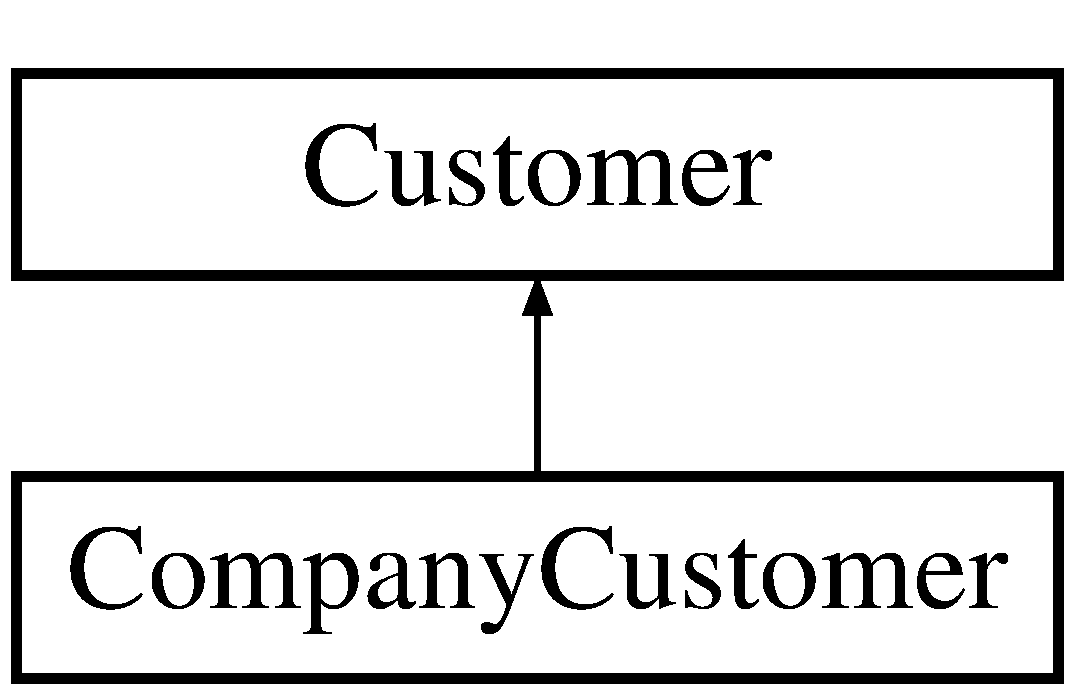
\includegraphics[height=2.000000cm]{classCompanyCustomer}
\end{center}
\end{figure}
\subsection*{Public Member Functions}
\begin{DoxyCompactItemize}
\item 
\hyperlink{classCompanyCustomer_a525a581a4b955657234bab5761ae2f02}{Company\+Customer} (unsigned int \hyperlink{classCustomer_a65ad3329532d5ad31e36f4ac81858e31}{nif}, string \hyperlink{classCustomer_a42c1c948fa0121c82b2725826d9f8300}{name}, string \hyperlink{classCustomer_a72d87951c1b76883390d00baf044cf2c}{address}, int \hyperlink{classCustomer_ad8c8d99b4c35f66a1a87b234c6078e0f}{phone\+Number}, double \hyperlink{classCompanyCustomer_a69dd60239a6ccfef6c444e64975fb5d7}{cost})
\item 
\hyperlink{classCompanyCustomer_af95c687f20e167f7df7e6fcee1493e7f}{Company\+Customer} (unsigned int \hyperlink{classCustomer_a65ad3329532d5ad31e36f4ac81858e31}{nif}, string \hyperlink{classCustomer_a42c1c948fa0121c82b2725826d9f8300}{name}, string \hyperlink{classCustomer_a72d87951c1b76883390d00baf044cf2c}{address}, int \hyperlink{classCustomer_ad8c8d99b4c35f66a1a87b234c6078e0f}{phone\+Number}, double \hyperlink{classCompanyCustomer_a69dd60239a6ccfef6c444e64975fb5d7}{cost}, \hyperlink{classVoucher}{Voucher} $\ast$\hyperlink{classCompanyCustomer_a19915d197c698ef79c608a6ca1f178fe}{voucher})
\item 
\hyperlink{classCompanyCustomer_afd96d1b12bbaf07317777b0736eb1d3f}{$\sim$\+Company\+Customer} ()
\item 
int \hyperlink{classCompanyCustomer_a4552ae519d7ba549979d7f67cfdec3fb}{get\+Cost} ()
\item 
float \hyperlink{classCompanyCustomer_aa9af04558e4c90df0c2379456ae7b626}{get\+Discount} ()
\item 
void \hyperlink{classCompanyCustomer_a20935ee3df903d3933c74e8bc2148402}{reset\+Cost} ()
\item 
void \hyperlink{classCompanyCustomer_a904197ef9475d4309ac41cc54a2ae5a3}{accumulate\+Service} (\hyperlink{classService}{Service} $\ast$service)
\item 
\hyperlink{classCustomer_adf157cb713398bb38163743659ec3049}{C\+U\+S\+T\+O\+M\+E\+R\+\_\+\+T\+Y\+PE} \hyperlink{classCompanyCustomer_a29b36593a5cc93f3c6d9f9372b261bba}{get\+Customer\+Type} ()
\item 
string \hyperlink{classCompanyCustomer_a43dcc60f21c2b48e4af587314653d94d}{get\+Information} ()
\item 
string \hyperlink{classCompanyCustomer_aae3bd828d590b136e6ca407ef6f47350}{to\+File\+Format} ()
\item 
\hyperlink{classVoucher}{Voucher} $\ast$ \hyperlink{classCompanyCustomer_a8cac3004028091378a2edb5cc211f1c8}{add\+Voucher} (\hyperlink{classVoucher}{Voucher} $\ast$\hyperlink{classCompanyCustomer_a19915d197c698ef79c608a6ca1f178fe}{voucher})
\end{DoxyCompactItemize}
\subsection*{Private Attributes}
\begin{DoxyCompactItemize}
\item 
double \hyperlink{classCompanyCustomer_a69dd60239a6ccfef6c444e64975fb5d7}{cost}
\item 
\hyperlink{classVoucher}{Voucher} $\ast$ \hyperlink{classCompanyCustomer_a19915d197c698ef79c608a6ca1f178fe}{voucher}
\end{DoxyCompactItemize}
\subsection*{Additional Inherited Members}


\subsection{Constructor \& Destructor Documentation}
\hypertarget{classCompanyCustomer_a525a581a4b955657234bab5761ae2f02}{}\label{classCompanyCustomer_a525a581a4b955657234bab5761ae2f02} 
\index{Company\+Customer@{Company\+Customer}!Company\+Customer@{Company\+Customer}}
\index{Company\+Customer@{Company\+Customer}!Company\+Customer@{Company\+Customer}}
\subsubsection{\texorpdfstring{Company\+Customer()}{CompanyCustomer()}\hspace{0.1cm}{\footnotesize\ttfamily [1/2]}}
{\footnotesize\ttfamily Company\+Customer\+::\+Company\+Customer (\begin{DoxyParamCaption}\item[{unsigned int}]{nif,  }\item[{string}]{name,  }\item[{string}]{address,  }\item[{int}]{phone\+Number,  }\item[{double}]{cost }\end{DoxyParamCaption})}

The constructor of the \hyperlink{classCompanyCustomer}{Company\+Customer} class, where the elements are initialized. As a new customer, at first the company don\textquotesingle{}t have vouchers. 
\begin{DoxyParams}{Parameters}
{\em nif} & customer nif \\
\hline
{\em name} & customer name \\
\hline
{\em address} & customer address \\
\hline
{\em phone\+Number} & customer phone number \\
\hline
{\em cost} & total value of cutomer services \\
\hline
\end{DoxyParams}
\hypertarget{classCompanyCustomer_af95c687f20e167f7df7e6fcee1493e7f}{}\label{classCompanyCustomer_af95c687f20e167f7df7e6fcee1493e7f} 
\index{Company\+Customer@{Company\+Customer}!Company\+Customer@{Company\+Customer}}
\index{Company\+Customer@{Company\+Customer}!Company\+Customer@{Company\+Customer}}
\subsubsection{\texorpdfstring{Company\+Customer()}{CompanyCustomer()}\hspace{0.1cm}{\footnotesize\ttfamily [2/2]}}
{\footnotesize\ttfamily Company\+Customer\+::\+Company\+Customer (\begin{DoxyParamCaption}\item[{unsigned int}]{nif,  }\item[{string}]{name,  }\item[{string}]{address,  }\item[{int}]{phone\+Number,  }\item[{double}]{cost,  }\item[{\hyperlink{classVoucher}{Voucher} $\ast$}]{voucher }\end{DoxyParamCaption})}

The constructor of the \hyperlink{classCompanyCustomer}{Company\+Customer} class, where the elements are initialized. 
\begin{DoxyParams}{Parameters}
{\em nif} & customer nif \\
\hline
{\em name} & customer name \\
\hline
{\em address} & customer address \\
\hline
{\em phone\+Number} & customer phone number \\
\hline
{\em cost} & total value of cutomer services \\
\hline
{\em voucher} & company customer voucher \\
\hline
\end{DoxyParams}
\hypertarget{classCompanyCustomer_afd96d1b12bbaf07317777b0736eb1d3f}{}\label{classCompanyCustomer_afd96d1b12bbaf07317777b0736eb1d3f} 
\index{Company\+Customer@{Company\+Customer}!````~Company\+Customer@{$\sim$\+Company\+Customer}}
\index{````~Company\+Customer@{$\sim$\+Company\+Customer}!Company\+Customer@{Company\+Customer}}
\subsubsection{\texorpdfstring{$\sim$\+Company\+Customer()}{~CompanyCustomer()}}
{\footnotesize\ttfamily Company\+Customer\+::$\sim$\+Company\+Customer (\begin{DoxyParamCaption}{ }\end{DoxyParamCaption})}

The destructor 

\subsection{Member Function Documentation}
\hypertarget{classCompanyCustomer_a904197ef9475d4309ac41cc54a2ae5a3}{}\label{classCompanyCustomer_a904197ef9475d4309ac41cc54a2ae5a3} 
\index{Company\+Customer@{Company\+Customer}!accumulate\+Service@{accumulate\+Service}}
\index{accumulate\+Service@{accumulate\+Service}!Company\+Customer@{Company\+Customer}}
\subsubsection{\texorpdfstring{accumulate\+Service()}{accumulateService()}}
{\footnotesize\ttfamily void Company\+Customer\+::accumulate\+Service (\begin{DoxyParamCaption}\item[{\hyperlink{classService}{Service} $\ast$}]{service }\end{DoxyParamCaption})\hspace{0.3cm}{\ttfamily [virtual]}}

This function adds to the cost the value of the service. 
\begin{DoxyParams}{Parameters}
{\em service} & available services \\
\hline
\end{DoxyParams}


Implements \hyperlink{classCustomer_ab42320f3e4d1c23e745ce901d30faf77}{Customer}.

\hypertarget{classCompanyCustomer_a8cac3004028091378a2edb5cc211f1c8}{}\label{classCompanyCustomer_a8cac3004028091378a2edb5cc211f1c8} 
\index{Company\+Customer@{Company\+Customer}!add\+Voucher@{add\+Voucher}}
\index{add\+Voucher@{add\+Voucher}!Company\+Customer@{Company\+Customer}}
\subsubsection{\texorpdfstring{add\+Voucher()}{addVoucher()}}
{\footnotesize\ttfamily \hyperlink{classVoucher}{Voucher} $\ast$ Company\+Customer\+::add\+Voucher (\begin{DoxyParamCaption}\item[{\hyperlink{classVoucher}{Voucher} $\ast$}]{voucher }\end{DoxyParamCaption})}

This function updates the deadline voucher. Please note that if we want to add, for example, 30 days to the voucher, they must be 30 calendar days. 
\begin{DoxyParams}{Parameters}
{\em voucher} & \hyperlink{classCompanyCustomer}{Company\+Customer} voucher \\
\hline
\end{DoxyParams}
\begin{DoxyReturn}{Returns}
the new voucher, this function can return the same voucher. 
\end{DoxyReturn}
\hypertarget{classCompanyCustomer_a4552ae519d7ba549979d7f67cfdec3fb}{}\label{classCompanyCustomer_a4552ae519d7ba549979d7f67cfdec3fb} 
\index{Company\+Customer@{Company\+Customer}!get\+Cost@{get\+Cost}}
\index{get\+Cost@{get\+Cost}!Company\+Customer@{Company\+Customer}}
\subsubsection{\texorpdfstring{get\+Cost()}{getCost()}}
{\footnotesize\ttfamily int Company\+Customer\+::get\+Cost (\begin{DoxyParamCaption}{ }\end{DoxyParamCaption})}

Cost is a private double of the \hyperlink{classCompanyCustomer}{Company\+Customer} class, we use \char`\"{}get\char`\"{} to be able to access this element in other classes. \begin{DoxyReturn}{Returns}
total value of cutomer services 
\end{DoxyReturn}
\hypertarget{classCompanyCustomer_a29b36593a5cc93f3c6d9f9372b261bba}{}\label{classCompanyCustomer_a29b36593a5cc93f3c6d9f9372b261bba} 
\index{Company\+Customer@{Company\+Customer}!get\+Customer\+Type@{get\+Customer\+Type}}
\index{get\+Customer\+Type@{get\+Customer\+Type}!Company\+Customer@{Company\+Customer}}
\subsubsection{\texorpdfstring{get\+Customer\+Type()}{getCustomerType()}}
{\footnotesize\ttfamily \hyperlink{classCustomer_adf157cb713398bb38163743659ec3049}{Customer\+::\+C\+U\+S\+T\+O\+M\+E\+R\+\_\+\+T\+Y\+PE} Company\+Customer\+::get\+Customer\+Type (\begin{DoxyParamCaption}{ }\end{DoxyParamCaption})\hspace{0.3cm}{\ttfamily [virtual]}}

This \char`\"{}enumerator\char`\"{} type restricts the types of existing customers 

Implements \hyperlink{classCustomer_a0353fcbdcb8ec729d95e9086df828e34}{Customer}.

\hypertarget{classCompanyCustomer_aa9af04558e4c90df0c2379456ae7b626}{}\label{classCompanyCustomer_aa9af04558e4c90df0c2379456ae7b626} 
\index{Company\+Customer@{Company\+Customer}!get\+Discount@{get\+Discount}}
\index{get\+Discount@{get\+Discount}!Company\+Customer@{Company\+Customer}}
\subsubsection{\texorpdfstring{get\+Discount()}{getDiscount()}}
{\footnotesize\ttfamily float Company\+Customer\+::get\+Discount (\begin{DoxyParamCaption}{ }\end{DoxyParamCaption})\hspace{0.3cm}{\ttfamily [virtual]}}

If the date of the voucher is already available, return the value of the voucher. \begin{DoxyReturn}{Returns}
value of company customer voucher 
\end{DoxyReturn}


Implements \hyperlink{classCustomer_a55df4714c5be2c2978069eda6bc32ace}{Customer}.

\hypertarget{classCompanyCustomer_a43dcc60f21c2b48e4af587314653d94d}{}\label{classCompanyCustomer_a43dcc60f21c2b48e4af587314653d94d} 
\index{Company\+Customer@{Company\+Customer}!get\+Information@{get\+Information}}
\index{get\+Information@{get\+Information}!Company\+Customer@{Company\+Customer}}
\subsubsection{\texorpdfstring{get\+Information()}{getInformation()}}
{\footnotesize\ttfamily string Company\+Customer\+::get\+Information (\begin{DoxyParamCaption}{ }\end{DoxyParamCaption})\hspace{0.3cm}{\ttfamily [virtual]}}

Get the information of a customer in line. \begin{DoxyReturn}{Returns}
string with the information of company customer service 
\end{DoxyReturn}


Reimplemented from \hyperlink{classCustomer_ae13da50be281b8f266f463a2166cad66}{Customer}.

\hypertarget{classCompanyCustomer_a20935ee3df903d3933c74e8bc2148402}{}\label{classCompanyCustomer_a20935ee3df903d3933c74e8bc2148402} 
\index{Company\+Customer@{Company\+Customer}!reset\+Cost@{reset\+Cost}}
\index{reset\+Cost@{reset\+Cost}!Company\+Customer@{Company\+Customer}}
\subsubsection{\texorpdfstring{reset\+Cost()}{resetCost()}}
{\footnotesize\ttfamily void Company\+Customer\+::reset\+Cost (\begin{DoxyParamCaption}{ }\end{DoxyParamCaption})}

Resets the company customer cost \hypertarget{classCompanyCustomer_aae3bd828d590b136e6ca407ef6f47350}{}\label{classCompanyCustomer_aae3bd828d590b136e6ca407ef6f47350} 
\index{Company\+Customer@{Company\+Customer}!to\+File\+Format@{to\+File\+Format}}
\index{to\+File\+Format@{to\+File\+Format}!Company\+Customer@{Company\+Customer}}
\subsubsection{\texorpdfstring{to\+File\+Format()}{toFileFormat()}}
{\footnotesize\ttfamily string Company\+Customer\+::to\+File\+Format (\begin{DoxyParamCaption}{ }\end{DoxyParamCaption})\hspace{0.3cm}{\ttfamily [virtual]}}

Put the information of a customer in the format needed. \begin{DoxyReturn}{Returns}
string with all information of the customer in the format needed. 
\end{DoxyReturn}


Reimplemented from \hyperlink{classCustomer_aa609cffee22046082003ea0ac3c191af}{Customer}.



\subsection{Member Data Documentation}
\hypertarget{classCompanyCustomer_a69dd60239a6ccfef6c444e64975fb5d7}{}\label{classCompanyCustomer_a69dd60239a6ccfef6c444e64975fb5d7} 
\index{Company\+Customer@{Company\+Customer}!cost@{cost}}
\index{cost@{cost}!Company\+Customer@{Company\+Customer}}
\subsubsection{\texorpdfstring{cost}{cost}}
{\footnotesize\ttfamily double Company\+Customer\+::cost\hspace{0.3cm}{\ttfamily [private]}}

\hypertarget{classCompanyCustomer_a19915d197c698ef79c608a6ca1f178fe}{}\label{classCompanyCustomer_a19915d197c698ef79c608a6ca1f178fe} 
\index{Company\+Customer@{Company\+Customer}!voucher@{voucher}}
\index{voucher@{voucher}!Company\+Customer@{Company\+Customer}}
\subsubsection{\texorpdfstring{voucher}{voucher}}
{\footnotesize\ttfamily \hyperlink{classVoucher}{Voucher}$\ast$ Company\+Customer\+::voucher\hspace{0.3cm}{\ttfamily [private]}}



The documentation for this class was generated from the following files\+:\begin{DoxyCompactItemize}
\item 
src/\hyperlink{CompanyCustomer_8h}{Company\+Customer.\+h}\item 
src/\hyperlink{CompanyCustomer_8cpp}{Company\+Customer.\+cpp}\end{DoxyCompactItemize}

\hypertarget{classCustomer}{}\section{Customer Class Reference}
\label{classCustomer}\index{Customer@{Customer}}


{\ttfamily \#include $<$Customer.\+h$>$}

Inheritance diagram for Customer\+:\begin{figure}[H]
\begin{center}
\leavevmode
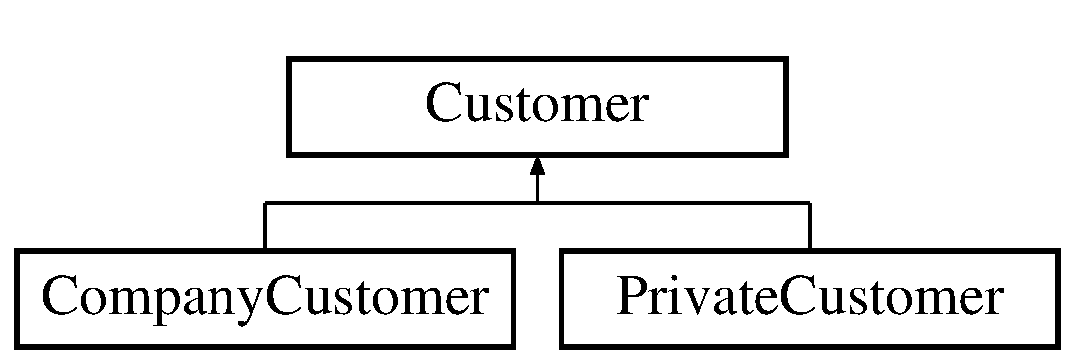
\includegraphics[height=2.000000cm]{classCustomer}
\end{center}
\end{figure}
\subsection*{Public Types}
\begin{DoxyCompactItemize}
\item 
enum \hyperlink{classCustomer_adf157cb713398bb38163743659ec3049}{C\+U\+S\+T\+O\+M\+E\+R\+\_\+\+T\+Y\+PE} \{ \hyperlink{classCustomer_adf157cb713398bb38163743659ec3049a6fd178caeb0cc24f8f4689d2d86de82b}{Company\+Customer}, 
\hyperlink{classCustomer_adf157cb713398bb38163743659ec3049a74cbae8b7e90efe986479e433ab9a840}{Private\+Customer}
 \}
\end{DoxyCompactItemize}
\subsection*{Public Member Functions}
\begin{DoxyCompactItemize}
\item 
\hyperlink{classCustomer_a2bb6a353723debbd4f7ef22540b50b11}{Customer} (unsigned int \hyperlink{classCustomer_a65ad3329532d5ad31e36f4ac81858e31}{nif}, string \hyperlink{classCustomer_a42c1c948fa0121c82b2725826d9f8300}{name}, string \hyperlink{classCustomer_a72d87951c1b76883390d00baf044cf2c}{address}, int \hyperlink{classCustomer_ad8c8d99b4c35f66a1a87b234c6078e0f}{phone\+Number})
\item 
virtual \hyperlink{classCustomer_ab93fb14683b0393b9c900109f77c2629}{$\sim$\+Customer} ()
\item 
string \hyperlink{classCustomer_a1bda0c5a9b2f4bf0c3314832e95f2566}{get\+Name} ()
\item 
string \hyperlink{classCustomer_aebd5a3862a90a21ec56198a69dbe7f34}{get\+Address} ()
\item 
int \hyperlink{classCustomer_ab64569e18c4b32d8f18f2711a5c124e3}{get\+Phone\+Number} ()
\item 
float \hyperlink{classCustomer_a10b0bb2b55a819b80c9e14cb19a7c566}{get\+Points} ()
\item 
unsigned int \hyperlink{classCustomer_a7dfa684a44a1e83f9dfaf0db8df32e14}{get\+Nif} () const
\item 
void \hyperlink{classCustomer_a7f9fdbe148a20c2ac310ea52f0a5311f}{set\+Name} (string)
\item 
void \hyperlink{classCustomer_aa955fe10dc1855ca78353b1677f76639}{set\+Address} (string)
\item 
void \hyperlink{classCustomer_a9260f17157643a0f7e57e233f8441e9b}{set\+Phone\+Number} (int)
\item 
virtual float \hyperlink{classCustomer_a55df4714c5be2c2978069eda6bc32ace}{get\+Discount} ()=0
\item 
virtual void \hyperlink{classCustomer_ab42320f3e4d1c23e745ce901d30faf77}{accumulate\+Service} (\hyperlink{classService}{Service} $\ast$)=0
\item 
virtual \hyperlink{classCustomer_adf157cb713398bb38163743659ec3049}{C\+U\+S\+T\+O\+M\+E\+R\+\_\+\+T\+Y\+PE} \hyperlink{classCustomer_a0353fcbdcb8ec729d95e9086df828e34}{get\+Customer\+Type} ()=0
\item 
virtual string \hyperlink{classCustomer_ae13da50be281b8f266f463a2166cad66}{get\+Information} ()
\item 
virtual string \hyperlink{classCustomer_aa609cffee22046082003ea0ac3c191af}{to\+File\+Format} ()
\end{DoxyCompactItemize}
\subsection*{Private Attributes}
\begin{DoxyCompactItemize}
\item 
string \hyperlink{classCustomer_a42c1c948fa0121c82b2725826d9f8300}{name}
\item 
string \hyperlink{classCustomer_a72d87951c1b76883390d00baf044cf2c}{address}
\item 
unsigned int \hyperlink{classCustomer_a65ad3329532d5ad31e36f4ac81858e31}{nif}
\item 
int \hyperlink{classCustomer_ad8c8d99b4c35f66a1a87b234c6078e0f}{phone\+Number}
\end{DoxyCompactItemize}


\subsection{Member Enumeration Documentation}
\hypertarget{classCustomer_adf157cb713398bb38163743659ec3049}{}\label{classCustomer_adf157cb713398bb38163743659ec3049} 
\index{Customer@{Customer}!C\+U\+S\+T\+O\+M\+E\+R\+\_\+\+T\+Y\+PE@{C\+U\+S\+T\+O\+M\+E\+R\+\_\+\+T\+Y\+PE}}
\index{C\+U\+S\+T\+O\+M\+E\+R\+\_\+\+T\+Y\+PE@{C\+U\+S\+T\+O\+M\+E\+R\+\_\+\+T\+Y\+PE}!Customer@{Customer}}
\subsubsection{\texorpdfstring{C\+U\+S\+T\+O\+M\+E\+R\+\_\+\+T\+Y\+PE}{CUSTOMER\_TYPE}}
{\footnotesize\ttfamily enum \hyperlink{classCustomer_adf157cb713398bb38163743659ec3049}{Customer\+::\+C\+U\+S\+T\+O\+M\+E\+R\+\_\+\+T\+Y\+PE}}

\begin{DoxyEnumFields}{Enumerator}
\raisebox{\heightof{T}}[0pt][0pt]{\index{Company\+Customer@{Company\+Customer}!Customer@{Customer}}\index{Customer@{Customer}!Company\+Customer@{Company\+Customer}}}\hypertarget{classCustomer_adf157cb713398bb38163743659ec3049a6fd178caeb0cc24f8f4689d2d86de82b}{}\label{classCustomer_adf157cb713398bb38163743659ec3049a6fd178caeb0cc24f8f4689d2d86de82b} 
Company\+Customer&\\
\hline

\raisebox{\heightof{T}}[0pt][0pt]{\index{Private\+Customer@{Private\+Customer}!Customer@{Customer}}\index{Customer@{Customer}!Private\+Customer@{Private\+Customer}}}\hypertarget{classCustomer_adf157cb713398bb38163743659ec3049a74cbae8b7e90efe986479e433ab9a840}{}\label{classCustomer_adf157cb713398bb38163743659ec3049a74cbae8b7e90efe986479e433ab9a840} 
Private\+Customer&\\
\hline

\end{DoxyEnumFields}


\subsection{Constructor \& Destructor Documentation}
\hypertarget{classCustomer_a2bb6a353723debbd4f7ef22540b50b11}{}\label{classCustomer_a2bb6a353723debbd4f7ef22540b50b11} 
\index{Customer@{Customer}!Customer@{Customer}}
\index{Customer@{Customer}!Customer@{Customer}}
\subsubsection{\texorpdfstring{Customer()}{Customer()}}
{\footnotesize\ttfamily Customer\+::\+Customer (\begin{DoxyParamCaption}\item[{unsigned int}]{nif,  }\item[{string}]{name,  }\item[{string}]{address,  }\item[{int}]{phone\+Number }\end{DoxyParamCaption})}

The constructor of the \hyperlink{classCustomer}{Customer} class, where the elements are initialized. 
\begin{DoxyParams}{Parameters}
{\em nif} & customer nif \\
\hline
{\em name} & customer name \\
\hline
{\em address} & customer address \\
\hline
{\em phone\+Number} & customer phone number \\
\hline
\end{DoxyParams}
\hypertarget{classCustomer_ab93fb14683b0393b9c900109f77c2629}{}\label{classCustomer_ab93fb14683b0393b9c900109f77c2629} 
\index{Customer@{Customer}!````~Customer@{$\sim$\+Customer}}
\index{````~Customer@{$\sim$\+Customer}!Customer@{Customer}}
\subsubsection{\texorpdfstring{$\sim$\+Customer()}{~Customer()}}
{\footnotesize\ttfamily Customer\+::$\sim$\+Customer (\begin{DoxyParamCaption}{ }\end{DoxyParamCaption})\hspace{0.3cm}{\ttfamily [virtual]}}

The destructor. 

\subsection{Member Function Documentation}
\hypertarget{classCustomer_ab42320f3e4d1c23e745ce901d30faf77}{}\label{classCustomer_ab42320f3e4d1c23e745ce901d30faf77} 
\index{Customer@{Customer}!accumulate\+Service@{accumulate\+Service}}
\index{accumulate\+Service@{accumulate\+Service}!Customer@{Customer}}
\subsubsection{\texorpdfstring{accumulate\+Service()}{accumulateService()}}
{\footnotesize\ttfamily virtual void Customer\+::accumulate\+Service (\begin{DoxyParamCaption}\item[{\hyperlink{classService}{Service} $\ast$}]{ }\end{DoxyParamCaption})\hspace{0.3cm}{\ttfamily [pure virtual]}}



Implemented in \hyperlink{classCompanyCustomer_a904197ef9475d4309ac41cc54a2ae5a3}{Company\+Customer}, and \hyperlink{classPrivateCustomer_a22e7d589398c26ac37973660f6e6f338}{Private\+Customer}.

\hypertarget{classCustomer_aebd5a3862a90a21ec56198a69dbe7f34}{}\label{classCustomer_aebd5a3862a90a21ec56198a69dbe7f34} 
\index{Customer@{Customer}!get\+Address@{get\+Address}}
\index{get\+Address@{get\+Address}!Customer@{Customer}}
\subsubsection{\texorpdfstring{get\+Address()}{getAddress()}}
{\footnotesize\ttfamily string Customer\+::get\+Address (\begin{DoxyParamCaption}{ }\end{DoxyParamCaption})}

Address is a private string of the \hyperlink{classCustomer}{Customer} class, we use \char`\"{}get\char`\"{} to be able to access this element in other classes. \begin{DoxyReturn}{Returns}
customer address 
\end{DoxyReturn}
\hypertarget{classCustomer_a0353fcbdcb8ec729d95e9086df828e34}{}\label{classCustomer_a0353fcbdcb8ec729d95e9086df828e34} 
\index{Customer@{Customer}!get\+Customer\+Type@{get\+Customer\+Type}}
\index{get\+Customer\+Type@{get\+Customer\+Type}!Customer@{Customer}}
\subsubsection{\texorpdfstring{get\+Customer\+Type()}{getCustomerType()}}
{\footnotesize\ttfamily virtual \hyperlink{classCustomer_adf157cb713398bb38163743659ec3049}{C\+U\+S\+T\+O\+M\+E\+R\+\_\+\+T\+Y\+PE} Customer\+::get\+Customer\+Type (\begin{DoxyParamCaption}{ }\end{DoxyParamCaption})\hspace{0.3cm}{\ttfamily [pure virtual]}}



Implemented in \hyperlink{classCompanyCustomer_a29b36593a5cc93f3c6d9f9372b261bba}{Company\+Customer}, and \hyperlink{classPrivateCustomer_a07d4d3e5995758b2407b8a81e35e579a}{Private\+Customer}.

\hypertarget{classCustomer_a55df4714c5be2c2978069eda6bc32ace}{}\label{classCustomer_a55df4714c5be2c2978069eda6bc32ace} 
\index{Customer@{Customer}!get\+Discount@{get\+Discount}}
\index{get\+Discount@{get\+Discount}!Customer@{Customer}}
\subsubsection{\texorpdfstring{get\+Discount()}{getDiscount()}}
{\footnotesize\ttfamily virtual float Customer\+::get\+Discount (\begin{DoxyParamCaption}{ }\end{DoxyParamCaption})\hspace{0.3cm}{\ttfamily [pure virtual]}}



Implemented in \hyperlink{classCompanyCustomer_aa9af04558e4c90df0c2379456ae7b626}{Company\+Customer}, and \hyperlink{classPrivateCustomer_a4757f4e3cb5e0e74891e8f1b37a07277}{Private\+Customer}.

\hypertarget{classCustomer_ae13da50be281b8f266f463a2166cad66}{}\label{classCustomer_ae13da50be281b8f266f463a2166cad66} 
\index{Customer@{Customer}!get\+Information@{get\+Information}}
\index{get\+Information@{get\+Information}!Customer@{Customer}}
\subsubsection{\texorpdfstring{get\+Information()}{getInformation()}}
{\footnotesize\ttfamily string Customer\+::get\+Information (\begin{DoxyParamCaption}{ }\end{DoxyParamCaption})\hspace{0.3cm}{\ttfamily [virtual]}}

Get a customer information in line with the customer table. \begin{DoxyReturn}{Returns}
a string with the customer information 
\end{DoxyReturn}


Reimplemented in \hyperlink{classCompanyCustomer_a43dcc60f21c2b48e4af587314653d94d}{Company\+Customer}, and \hyperlink{classPrivateCustomer_afcf22c4a25e9c961d045aa5a0d8d9fd2}{Private\+Customer}.

\hypertarget{classCustomer_a1bda0c5a9b2f4bf0c3314832e95f2566}{}\label{classCustomer_a1bda0c5a9b2f4bf0c3314832e95f2566} 
\index{Customer@{Customer}!get\+Name@{get\+Name}}
\index{get\+Name@{get\+Name}!Customer@{Customer}}
\subsubsection{\texorpdfstring{get\+Name()}{getName()}}
{\footnotesize\ttfamily string Customer\+::get\+Name (\begin{DoxyParamCaption}{ }\end{DoxyParamCaption})}

Name is a private string of the \hyperlink{classCustomer}{Customer} class, we use \char`\"{}get\char`\"{} to be able to access this element in other classes. \begin{DoxyReturn}{Returns}
customer name 
\end{DoxyReturn}
\hypertarget{classCustomer_a7dfa684a44a1e83f9dfaf0db8df32e14}{}\label{classCustomer_a7dfa684a44a1e83f9dfaf0db8df32e14} 
\index{Customer@{Customer}!get\+Nif@{get\+Nif}}
\index{get\+Nif@{get\+Nif}!Customer@{Customer}}
\subsubsection{\texorpdfstring{get\+Nif()}{getNif()}}
{\footnotesize\ttfamily unsigned int Customer\+::get\+Nif (\begin{DoxyParamCaption}{ }\end{DoxyParamCaption}) const}

Nif is a private unsigned integer of the \hyperlink{classCustomer}{Customer} class, we use \char`\"{}get\char`\"{} to be able to access this element in other classes. \begin{DoxyReturn}{Returns}
customer nif 
\end{DoxyReturn}
\hypertarget{classCustomer_ab64569e18c4b32d8f18f2711a5c124e3}{}\label{classCustomer_ab64569e18c4b32d8f18f2711a5c124e3} 
\index{Customer@{Customer}!get\+Phone\+Number@{get\+Phone\+Number}}
\index{get\+Phone\+Number@{get\+Phone\+Number}!Customer@{Customer}}
\subsubsection{\texorpdfstring{get\+Phone\+Number()}{getPhoneNumber()}}
{\footnotesize\ttfamily int Customer\+::get\+Phone\+Number (\begin{DoxyParamCaption}{ }\end{DoxyParamCaption})}

Phone\+Number is a private integer of the \hyperlink{classCustomer}{Customer} class, we use \char`\"{}get\char`\"{} to be able to access this element in other classes. \begin{DoxyReturn}{Returns}
customer phone number 
\end{DoxyReturn}
\hypertarget{classCustomer_a10b0bb2b55a819b80c9e14cb19a7c566}{}\label{classCustomer_a10b0bb2b55a819b80c9e14cb19a7c566} 
\index{Customer@{Customer}!get\+Points@{get\+Points}}
\index{get\+Points@{get\+Points}!Customer@{Customer}}
\subsubsection{\texorpdfstring{get\+Points()}{getPoints()}}
{\footnotesize\ttfamily float Customer\+::get\+Points (\begin{DoxyParamCaption}{ }\end{DoxyParamCaption})}

\hypertarget{classCustomer_aa955fe10dc1855ca78353b1677f76639}{}\label{classCustomer_aa955fe10dc1855ca78353b1677f76639} 
\index{Customer@{Customer}!set\+Address@{set\+Address}}
\index{set\+Address@{set\+Address}!Customer@{Customer}}
\subsubsection{\texorpdfstring{set\+Address()}{setAddress()}}
{\footnotesize\ttfamily void Customer\+::set\+Address (\begin{DoxyParamCaption}\item[{string}]{address }\end{DoxyParamCaption})}

Set the customer address. 
\begin{DoxyParams}{Parameters}
{\em customer} & address \\
\hline
\end{DoxyParams}
\hypertarget{classCustomer_a7f9fdbe148a20c2ac310ea52f0a5311f}{}\label{classCustomer_a7f9fdbe148a20c2ac310ea52f0a5311f} 
\index{Customer@{Customer}!set\+Name@{set\+Name}}
\index{set\+Name@{set\+Name}!Customer@{Customer}}
\subsubsection{\texorpdfstring{set\+Name()}{setName()}}
{\footnotesize\ttfamily void Customer\+::set\+Name (\begin{DoxyParamCaption}\item[{string}]{name }\end{DoxyParamCaption})}

Set the customer name. 
\begin{DoxyParams}{Parameters}
{\em customer} & name \\
\hline
\end{DoxyParams}
\hypertarget{classCustomer_a9260f17157643a0f7e57e233f8441e9b}{}\label{classCustomer_a9260f17157643a0f7e57e233f8441e9b} 
\index{Customer@{Customer}!set\+Phone\+Number@{set\+Phone\+Number}}
\index{set\+Phone\+Number@{set\+Phone\+Number}!Customer@{Customer}}
\subsubsection{\texorpdfstring{set\+Phone\+Number()}{setPhoneNumber()}}
{\footnotesize\ttfamily void Customer\+::set\+Phone\+Number (\begin{DoxyParamCaption}\item[{int}]{phone\+Number }\end{DoxyParamCaption})}

Set the customer phone number. 
\begin{DoxyParams}{Parameters}
{\em customer} & phone number \\
\hline
\end{DoxyParams}
\hypertarget{classCustomer_aa609cffee22046082003ea0ac3c191af}{}\label{classCustomer_aa609cffee22046082003ea0ac3c191af} 
\index{Customer@{Customer}!to\+File\+Format@{to\+File\+Format}}
\index{to\+File\+Format@{to\+File\+Format}!Customer@{Customer}}
\subsubsection{\texorpdfstring{to\+File\+Format()}{toFileFormat()}}
{\footnotesize\ttfamily string Customer\+::to\+File\+Format (\begin{DoxyParamCaption}{ }\end{DoxyParamCaption})\hspace{0.3cm}{\ttfamily [virtual]}}

Returns a string with all information of the customer in the format needed. \begin{DoxyReturn}{Returns}
a string with the customer information in the format needed 
\end{DoxyReturn}


Reimplemented in \hyperlink{classCompanyCustomer_aae3bd828d590b136e6ca407ef6f47350}{Company\+Customer}, and \hyperlink{classPrivateCustomer_adb678cbc09d9e4a8e9e4ab0d556b8b6c}{Private\+Customer}.



\subsection{Member Data Documentation}
\hypertarget{classCustomer_a72d87951c1b76883390d00baf044cf2c}{}\label{classCustomer_a72d87951c1b76883390d00baf044cf2c} 
\index{Customer@{Customer}!address@{address}}
\index{address@{address}!Customer@{Customer}}
\subsubsection{\texorpdfstring{address}{address}}
{\footnotesize\ttfamily string Customer\+::address\hspace{0.3cm}{\ttfamily [private]}}

\hypertarget{classCustomer_a42c1c948fa0121c82b2725826d9f8300}{}\label{classCustomer_a42c1c948fa0121c82b2725826d9f8300} 
\index{Customer@{Customer}!name@{name}}
\index{name@{name}!Customer@{Customer}}
\subsubsection{\texorpdfstring{name}{name}}
{\footnotesize\ttfamily string Customer\+::name\hspace{0.3cm}{\ttfamily [private]}}

\hypertarget{classCustomer_a65ad3329532d5ad31e36f4ac81858e31}{}\label{classCustomer_a65ad3329532d5ad31e36f4ac81858e31} 
\index{Customer@{Customer}!nif@{nif}}
\index{nif@{nif}!Customer@{Customer}}
\subsubsection{\texorpdfstring{nif}{nif}}
{\footnotesize\ttfamily unsigned int Customer\+::nif\hspace{0.3cm}{\ttfamily [private]}}

\hypertarget{classCustomer_ad8c8d99b4c35f66a1a87b234c6078e0f}{}\label{classCustomer_ad8c8d99b4c35f66a1a87b234c6078e0f} 
\index{Customer@{Customer}!phone\+Number@{phone\+Number}}
\index{phone\+Number@{phone\+Number}!Customer@{Customer}}
\subsubsection{\texorpdfstring{phone\+Number}{phoneNumber}}
{\footnotesize\ttfamily int Customer\+::phone\+Number\hspace{0.3cm}{\ttfamily [private]}}



The documentation for this class was generated from the following files\+:\begin{DoxyCompactItemize}
\item 
src/\hyperlink{Customer_8h}{Customer.\+h}\item 
src/\hyperlink{Customer_8cpp}{Customer.\+cpp}\end{DoxyCompactItemize}

\hypertarget{classDate}{}\section{Date Class Reference}
\label{classDate}\index{Date@{Date}}


{\ttfamily \#include $<$Date.\+h$>$}

\subsection*{Public Member Functions}
\begin{DoxyCompactItemize}
\item 
\hyperlink{classDate_a4e59ed4ba66eec61c27460c5d09fa1bd}{Date} ()
\item 
\hyperlink{classDate_a28c6604a0f8ed8216becf24abc20cf5b}{Date} (unsigned int \hyperlink{classDate_a6c498dee79268960e000ec3deaa555ac}{day}, unsigned int \hyperlink{classDate_af48402007169fe01234fe9bb9e7a1d2c}{month}, unsigned int \hyperlink{classDate_afc014a1ae62e56be473144050201e62a}{year})
\item 
\hyperlink{classDate_a2ca1c1b9d156db59120f5a3727df134c}{Date} (string day\+Month\+Year)
\item 
void \hyperlink{classDate_a1299c7e1f0080304f082a9225a743957}{set\+Year} (unsigned int \hyperlink{classDate_afc014a1ae62e56be473144050201e62a}{year})
\item 
void \hyperlink{classDate_aa83b79359070012ab58ff99abeb34340}{set\+Month} (unsigned int \hyperlink{classDate_af48402007169fe01234fe9bb9e7a1d2c}{month})
\item 
void \hyperlink{classDate_a18dc2bd52ab8adcca331f66c27ed6623}{set\+Day} (unsigned int \hyperlink{classDate_a6c498dee79268960e000ec3deaa555ac}{day})
\item 
void \hyperlink{classDate_abbd3c22e63d9fb3fbb1a34e5614aab22}{set\+Date} (string date)
\item 
unsigned int \hyperlink{classDate_a597b505c264a24d34369c43119fc4e6e}{get\+Year} () const
\item 
unsigned int \hyperlink{classDate_a6152596dcf2e1e78e2095ea518de59e7}{get\+Month} () const
\item 
unsigned int \hyperlink{classDate_a13855b25efb79eaf7dccf08555421a1d}{get\+Day} () const
\item 
string \hyperlink{classDate_a00fe723e95db62fed0990f5b28f8baf2}{date\+As\+String} ()
\item 
void \hyperlink{classDate_addaed921af229dffeb35ef7ef30bff29}{show} ()
\item 
bool \hyperlink{classDate_a7d9aaa9db591413e21c8b85fdae130ad}{is\+Valid} ()
\item 
bool \hyperlink{classDate_a4b933e8c9e1a5853918ad88eb2fc2dae}{operator==} (const \hyperlink{classDate}{Date} \&date)
\item 
bool \hyperlink{classDate_a4a291faa73653c0a14981db2dee21678}{operator$>$=} (const \hyperlink{classDate}{Date} \&date)
\item 
bool \hyperlink{classDate_ab0656086910c8debe2a1fb5d2ae197ba}{operator$<$=} (const \hyperlink{classDate}{Date} \&date)
\item 
\hyperlink{classDate}{Date} \hyperlink{classDate_a2a6e45e4a2de73d7ec7b9227442c4a3f}{get\+Next\+Month} ()
\end{DoxyCompactItemize}
\subsection*{Private Member Functions}
\begin{DoxyCompactItemize}
\item 
bool \hyperlink{classDate_ab83816d7572d1a15c6e86378b82a54f0}{is\+Leap\+Year} ()
\item 
unsigned int \hyperlink{classDate_a9cd38c6d1cc0e326baef6ab8a25029b8}{n\+Days} ()
\end{DoxyCompactItemize}
\subsection*{Private Attributes}
\begin{DoxyCompactItemize}
\item 
unsigned int \hyperlink{classDate_afc014a1ae62e56be473144050201e62a}{year}
\item 
unsigned int \hyperlink{classDate_af48402007169fe01234fe9bb9e7a1d2c}{month}
\item 
unsigned int \hyperlink{classDate_a6c498dee79268960e000ec3deaa555ac}{day}
\end{DoxyCompactItemize}


\subsection{Constructor \& Destructor Documentation}
\hypertarget{classDate_a4e59ed4ba66eec61c27460c5d09fa1bd}{}\label{classDate_a4e59ed4ba66eec61c27460c5d09fa1bd} 
\index{Date@{Date}!Date@{Date}}
\index{Date@{Date}!Date@{Date}}
\subsubsection{\texorpdfstring{Date()}{Date()}\hspace{0.1cm}{\footnotesize\ttfamily [1/3]}}
{\footnotesize\ttfamily Date\+::\+Date (\begin{DoxyParamCaption}{ }\end{DoxyParamCaption})}

Empty constructor. \hypertarget{classDate_a28c6604a0f8ed8216becf24abc20cf5b}{}\label{classDate_a28c6604a0f8ed8216becf24abc20cf5b} 
\index{Date@{Date}!Date@{Date}}
\index{Date@{Date}!Date@{Date}}
\subsubsection{\texorpdfstring{Date()}{Date()}\hspace{0.1cm}{\footnotesize\ttfamily [2/3]}}
{\footnotesize\ttfamily Date\+::\+Date (\begin{DoxyParamCaption}\item[{unsigned int}]{day,  }\item[{unsigned int}]{month,  }\item[{unsigned int}]{year }\end{DoxyParamCaption})}

The constructor of the \hyperlink{classDate}{Date} class, where the elements are initialized. 
\begin{DoxyParams}{Parameters}
{\em day} & day of the date \\
\hline
{\em moth} & month of the date \\
\hline
{\em year} & year of the date \\
\hline
\end{DoxyParams}
\hypertarget{classDate_a2ca1c1b9d156db59120f5a3727df134c}{}\label{classDate_a2ca1c1b9d156db59120f5a3727df134c} 
\index{Date@{Date}!Date@{Date}}
\index{Date@{Date}!Date@{Date}}
\subsubsection{\texorpdfstring{Date()}{Date()}\hspace{0.1cm}{\footnotesize\ttfamily [3/3]}}
{\footnotesize\ttfamily Date\+::\+Date (\begin{DoxyParamCaption}\item[{string}]{day\+Month\+Year }\end{DoxyParamCaption})}

The constructor of the \hyperlink{classDate}{Date} class, where the elements are initialized. This constructor receive the date as a string. 
\begin{DoxyParams}{Parameters}
{\em day\+Month\+Year} & the date string \\
\hline
\end{DoxyParams}


\subsection{Member Function Documentation}
\hypertarget{classDate_a00fe723e95db62fed0990f5b28f8baf2}{}\label{classDate_a00fe723e95db62fed0990f5b28f8baf2} 
\index{Date@{Date}!date\+As\+String@{date\+As\+String}}
\index{date\+As\+String@{date\+As\+String}!Date@{Date}}
\subsubsection{\texorpdfstring{date\+As\+String()}{dateAsString()}}
{\footnotesize\ttfamily string Date\+::date\+As\+String (\begin{DoxyParamCaption}{ }\end{DoxyParamCaption})}

This function convert a string(who is a date) to the following format\+: day/moth/year. \begin{DoxyReturn}{Returns}
a string with the date in the format needed 
\end{DoxyReturn}
\hypertarget{classDate_a13855b25efb79eaf7dccf08555421a1d}{}\label{classDate_a13855b25efb79eaf7dccf08555421a1d} 
\index{Date@{Date}!get\+Day@{get\+Day}}
\index{get\+Day@{get\+Day}!Date@{Date}}
\subsubsection{\texorpdfstring{get\+Day()}{getDay()}}
{\footnotesize\ttfamily unsigned int Date\+::get\+Day (\begin{DoxyParamCaption}{ }\end{DoxyParamCaption}) const}

Day is a private unsigned integer of the \hyperlink{classDate}{Date} class, we use \char`\"{}get\char`\"{} to be able to access this element in other classes. \hypertarget{classDate_a6152596dcf2e1e78e2095ea518de59e7}{}\label{classDate_a6152596dcf2e1e78e2095ea518de59e7} 
\index{Date@{Date}!get\+Month@{get\+Month}}
\index{get\+Month@{get\+Month}!Date@{Date}}
\subsubsection{\texorpdfstring{get\+Month()}{getMonth()}}
{\footnotesize\ttfamily unsigned int Date\+::get\+Month (\begin{DoxyParamCaption}{ }\end{DoxyParamCaption}) const}

Month is a private unsigned integer of the \hyperlink{classDate}{Date} class, we use \char`\"{}get\char`\"{} to be able to access this element in other classes. \hypertarget{classDate_a2a6e45e4a2de73d7ec7b9227442c4a3f}{}\label{classDate_a2a6e45e4a2de73d7ec7b9227442c4a3f} 
\index{Date@{Date}!get\+Next\+Month@{get\+Next\+Month}}
\index{get\+Next\+Month@{get\+Next\+Month}!Date@{Date}}
\subsubsection{\texorpdfstring{get\+Next\+Month()}{getNextMonth()}}
{\footnotesize\ttfamily \hyperlink{classDate}{Date} Date\+::get\+Next\+Month (\begin{DoxyParamCaption}{ }\end{DoxyParamCaption})}

Get the next month of a date and update the date. \begin{DoxyReturn}{Returns}
the new date 
\end{DoxyReturn}
\hypertarget{classDate_a597b505c264a24d34369c43119fc4e6e}{}\label{classDate_a597b505c264a24d34369c43119fc4e6e} 
\index{Date@{Date}!get\+Year@{get\+Year}}
\index{get\+Year@{get\+Year}!Date@{Date}}
\subsubsection{\texorpdfstring{get\+Year()}{getYear()}}
{\footnotesize\ttfamily unsigned int Date\+::get\+Year (\begin{DoxyParamCaption}{ }\end{DoxyParamCaption}) const}

Year is a private unsigned integer of the \hyperlink{classDate}{Date} class, we use \char`\"{}get\char`\"{} to be able to access this element in other classes. \hypertarget{classDate_ab83816d7572d1a15c6e86378b82a54f0}{}\label{classDate_ab83816d7572d1a15c6e86378b82a54f0} 
\index{Date@{Date}!is\+Leap\+Year@{is\+Leap\+Year}}
\index{is\+Leap\+Year@{is\+Leap\+Year}!Date@{Date}}
\subsubsection{\texorpdfstring{is\+Leap\+Year()}{isLeapYear()}}
{\footnotesize\ttfamily bool Date\+::is\+Leap\+Year (\begin{DoxyParamCaption}{ }\end{DoxyParamCaption})\hspace{0.3cm}{\ttfamily [private]}}

This function checks if the year is leap. \begin{DoxyReturn}{Returns}
if the year is leap 
\end{DoxyReturn}
\hypertarget{classDate_a7d9aaa9db591413e21c8b85fdae130ad}{}\label{classDate_a7d9aaa9db591413e21c8b85fdae130ad} 
\index{Date@{Date}!is\+Valid@{is\+Valid}}
\index{is\+Valid@{is\+Valid}!Date@{Date}}
\subsubsection{\texorpdfstring{is\+Valid()}{isValid()}}
{\footnotesize\ttfamily bool Date\+::is\+Valid (\begin{DoxyParamCaption}{ }\end{DoxyParamCaption})}

This function verify is a date is valid. \begin{DoxyReturn}{Returns}
if the date is valid 
\end{DoxyReturn}
\hypertarget{classDate_a9cd38c6d1cc0e326baef6ab8a25029b8}{}\label{classDate_a9cd38c6d1cc0e326baef6ab8a25029b8} 
\index{Date@{Date}!n\+Days@{n\+Days}}
\index{n\+Days@{n\+Days}!Date@{Date}}
\subsubsection{\texorpdfstring{n\+Days()}{nDays()}}
{\footnotesize\ttfamily unsigned int Date\+::n\+Days (\begin{DoxyParamCaption}{ }\end{DoxyParamCaption})\hspace{0.3cm}{\ttfamily [private]}}

This function verify if the day is valid, according to the month days. \begin{DoxyReturn}{Returns}
the number of days in a month 
\end{DoxyReturn}
\hypertarget{classDate_ab0656086910c8debe2a1fb5d2ae197ba}{}\label{classDate_ab0656086910c8debe2a1fb5d2ae197ba} 
\index{Date@{Date}!operator$<$=@{operator$<$=}}
\index{operator$<$=@{operator$<$=}!Date@{Date}}
\subsubsection{\texorpdfstring{operator$<$=()}{operator<=()}}
{\footnotesize\ttfamily bool Date\+::operator$<$= (\begin{DoxyParamCaption}\item[{const \hyperlink{classDate}{Date} \&}]{date }\end{DoxyParamCaption})}

Check if one date is equal to or less than another. 
\begin{DoxyParams}{Parameters}
{\em date} & the second date to compare \\
\hline
\end{DoxyParams}
\begin{DoxyReturn}{Returns}
if one date is equal to or less than another 
\end{DoxyReturn}
\hypertarget{classDate_a4b933e8c9e1a5853918ad88eb2fc2dae}{}\label{classDate_a4b933e8c9e1a5853918ad88eb2fc2dae} 
\index{Date@{Date}!operator==@{operator==}}
\index{operator==@{operator==}!Date@{Date}}
\subsubsection{\texorpdfstring{operator==()}{operator==()}}
{\footnotesize\ttfamily bool Date\+::operator== (\begin{DoxyParamCaption}\item[{const \hyperlink{classDate}{Date} \&}]{date }\end{DoxyParamCaption})}

Check if dates are equal. 
\begin{DoxyParams}{Parameters}
{\em date} & the second date to compare \\
\hline
\end{DoxyParams}
\begin{DoxyReturn}{Returns}
if two dates are equal 
\end{DoxyReturn}
\hypertarget{classDate_a4a291faa73653c0a14981db2dee21678}{}\label{classDate_a4a291faa73653c0a14981db2dee21678} 
\index{Date@{Date}!operator$>$=@{operator$>$=}}
\index{operator$>$=@{operator$>$=}!Date@{Date}}
\subsubsection{\texorpdfstring{operator$>$=()}{operator>=()}}
{\footnotesize\ttfamily bool Date\+::operator$>$= (\begin{DoxyParamCaption}\item[{const \hyperlink{classDate}{Date} \&}]{date }\end{DoxyParamCaption})}

Check if one date is equal to or greater than another. 
\begin{DoxyParams}{Parameters}
{\em date} & the second date to compare \\
\hline
\end{DoxyParams}
\begin{DoxyReturn}{Returns}
if one date is equal to or greater than another 
\end{DoxyReturn}
\hypertarget{classDate_abbd3c22e63d9fb3fbb1a34e5614aab22}{}\label{classDate_abbd3c22e63d9fb3fbb1a34e5614aab22} 
\index{Date@{Date}!set\+Date@{set\+Date}}
\index{set\+Date@{set\+Date}!Date@{Date}}
\subsubsection{\texorpdfstring{set\+Date()}{setDate()}}
{\footnotesize\ttfamily void Date\+::set\+Date (\begin{DoxyParamCaption}\item[{string}]{date }\end{DoxyParamCaption})}

Set the date If day, month or year are not valid, make whole date invalid. 
\begin{DoxyParams}{Parameters}
{\em date} & date \\
\hline
\end{DoxyParams}
\hypertarget{classDate_a18dc2bd52ab8adcca331f66c27ed6623}{}\label{classDate_a18dc2bd52ab8adcca331f66c27ed6623} 
\index{Date@{Date}!set\+Day@{set\+Day}}
\index{set\+Day@{set\+Day}!Date@{Date}}
\subsubsection{\texorpdfstring{set\+Day()}{setDay()}}
{\footnotesize\ttfamily void Date\+::set\+Day (\begin{DoxyParamCaption}\item[{unsigned int}]{day }\end{DoxyParamCaption})}

Set the day of the date 
\begin{DoxyParams}{Parameters}
{\em day} & of the date \\
\hline
\end{DoxyParams}
\hypertarget{classDate_aa83b79359070012ab58ff99abeb34340}{}\label{classDate_aa83b79359070012ab58ff99abeb34340} 
\index{Date@{Date}!set\+Month@{set\+Month}}
\index{set\+Month@{set\+Month}!Date@{Date}}
\subsubsection{\texorpdfstring{set\+Month()}{setMonth()}}
{\footnotesize\ttfamily void Date\+::set\+Month (\begin{DoxyParamCaption}\item[{unsigned int}]{month }\end{DoxyParamCaption})}

Set the month of the date 
\begin{DoxyParams}{Parameters}
{\em month} & of the date \\
\hline
\end{DoxyParams}
\hypertarget{classDate_a1299c7e1f0080304f082a9225a743957}{}\label{classDate_a1299c7e1f0080304f082a9225a743957} 
\index{Date@{Date}!set\+Year@{set\+Year}}
\index{set\+Year@{set\+Year}!Date@{Date}}
\subsubsection{\texorpdfstring{set\+Year()}{setYear()}}
{\footnotesize\ttfamily void Date\+::set\+Year (\begin{DoxyParamCaption}\item[{unsigned int}]{year }\end{DoxyParamCaption})}

Set the year of the date 
\begin{DoxyParams}{Parameters}
{\em year} & year of the date \\
\hline
\end{DoxyParams}
\hypertarget{classDate_addaed921af229dffeb35ef7ef30bff29}{}\label{classDate_addaed921af229dffeb35ef7ef30bff29} 
\index{Date@{Date}!show@{show}}
\index{show@{show}!Date@{Date}}
\subsubsection{\texorpdfstring{show()}{show()}}
{\footnotesize\ttfamily void Date\+::show (\begin{DoxyParamCaption}{ }\end{DoxyParamCaption})}

This function shows a date with the following format\+: day/moth/year. 

\subsection{Member Data Documentation}
\hypertarget{classDate_a6c498dee79268960e000ec3deaa555ac}{}\label{classDate_a6c498dee79268960e000ec3deaa555ac} 
\index{Date@{Date}!day@{day}}
\index{day@{day}!Date@{Date}}
\subsubsection{\texorpdfstring{day}{day}}
{\footnotesize\ttfamily unsigned int Date\+::day\hspace{0.3cm}{\ttfamily [private]}}

\hypertarget{classDate_af48402007169fe01234fe9bb9e7a1d2c}{}\label{classDate_af48402007169fe01234fe9bb9e7a1d2c} 
\index{Date@{Date}!month@{month}}
\index{month@{month}!Date@{Date}}
\subsubsection{\texorpdfstring{month}{month}}
{\footnotesize\ttfamily unsigned int Date\+::month\hspace{0.3cm}{\ttfamily [private]}}

\hypertarget{classDate_afc014a1ae62e56be473144050201e62a}{}\label{classDate_afc014a1ae62e56be473144050201e62a} 
\index{Date@{Date}!year@{year}}
\index{year@{year}!Date@{Date}}
\subsubsection{\texorpdfstring{year}{year}}
{\footnotesize\ttfamily unsigned int Date\+::year\hspace{0.3cm}{\ttfamily [private]}}



The documentation for this class was generated from the following files\+:\begin{DoxyCompactItemize}
\item 
src/\hyperlink{Date_8h}{Date.\+h}\item 
src/\hyperlink{Date_8cpp}{Date.\+cpp}\end{DoxyCompactItemize}

\hypertarget{classInvalidDistanceException}{}\section{Invalid\+Distance\+Exception Class Reference}
\label{classInvalidDistanceException}\index{Invalid\+Distance\+Exception@{Invalid\+Distance\+Exception}}


{\ttfamily \#include $<$Route.\+h$>$}

\subsection*{Friends}
\begin{DoxyCompactItemize}
\item 
ostream \& \hyperlink{classInvalidDistanceException_a66a9d7f1c3f796754d1c8dedc34697da}{operator$<$$<$} (std\+::ostream \&out, \hyperlink{classInvalidDistanceException}{Invalid\+Distance\+Exception} \&e)
\end{DoxyCompactItemize}


\subsection{Friends And Related Function Documentation}
\hypertarget{classInvalidDistanceException_a66a9d7f1c3f796754d1c8dedc34697da}{}\label{classInvalidDistanceException_a66a9d7f1c3f796754d1c8dedc34697da} 
\index{Invalid\+Distance\+Exception@{Invalid\+Distance\+Exception}!operator$<$$<$@{operator$<$$<$}}
\index{operator$<$$<$@{operator$<$$<$}!Invalid\+Distance\+Exception@{Invalid\+Distance\+Exception}}
\subsubsection{\texorpdfstring{operator$<$$<$}{operator<<}}
{\footnotesize\ttfamily ostream\& operator$<$$<$ (\begin{DoxyParamCaption}\item[{std\+::ostream \&}]{out,  }\item[{\hyperlink{classInvalidDistanceException}{Invalid\+Distance\+Exception} \&}]{e }\end{DoxyParamCaption})\hspace{0.3cm}{\ttfamily [friend]}}



The documentation for this class was generated from the following file\+:\begin{DoxyCompactItemize}
\item 
src/\hyperlink{Route_8h}{Route.\+h}\end{DoxyCompactItemize}

\hypertarget{classInvalidExpectedTimeException}{}\section{Invalid\+Expected\+Time\+Exception Class Reference}
\label{classInvalidExpectedTimeException}\index{Invalid\+Expected\+Time\+Exception@{Invalid\+Expected\+Time\+Exception}}


{\ttfamily \#include $<$Route.\+h$>$}

\subsection*{Friends}
\begin{DoxyCompactItemize}
\item 
ostream \& \hyperlink{classInvalidExpectedTimeException_ade435a7c98c3c9fa94bb27930e4874cf}{operator$<$$<$} (std\+::ostream \&out, \hyperlink{classInvalidExpectedTimeException}{Invalid\+Expected\+Time\+Exception} \&e)
\end{DoxyCompactItemize}


\subsection{Friends And Related Function Documentation}
\hypertarget{classInvalidExpectedTimeException_ade435a7c98c3c9fa94bb27930e4874cf}{}\label{classInvalidExpectedTimeException_ade435a7c98c3c9fa94bb27930e4874cf} 
\index{Invalid\+Expected\+Time\+Exception@{Invalid\+Expected\+Time\+Exception}!operator$<$$<$@{operator$<$$<$}}
\index{operator$<$$<$@{operator$<$$<$}!Invalid\+Expected\+Time\+Exception@{Invalid\+Expected\+Time\+Exception}}
\subsubsection{\texorpdfstring{operator$<$$<$}{operator<<}}
{\footnotesize\ttfamily ostream\& operator$<$$<$ (\begin{DoxyParamCaption}\item[{std\+::ostream \&}]{out,  }\item[{\hyperlink{classInvalidExpectedTimeException}{Invalid\+Expected\+Time\+Exception} \&}]{e }\end{DoxyParamCaption})\hspace{0.3cm}{\ttfamily [friend]}}



The documentation for this class was generated from the following file\+:\begin{DoxyCompactItemize}
\item 
src/\hyperlink{Route_8h}{Route.\+h}\end{DoxyCompactItemize}

\hypertarget{classInvalidNifException}{}\section{Invalid\+Nif\+Exception Class Reference}
\label{classInvalidNifException}\index{Invalid\+Nif\+Exception@{Invalid\+Nif\+Exception}}


{\ttfamily \#include $<$Customer.\+h$>$}

\subsection*{Friends}
\begin{DoxyCompactItemize}
\item 
ostream \& \hyperlink{classInvalidNifException_a0fda405ea9244e1120b812bdd03b7fd8}{operator$<$$<$} (std\+::ostream \&out, \hyperlink{classInvalidNifException}{Invalid\+Nif\+Exception} \&e)
\end{DoxyCompactItemize}


\subsection{Friends And Related Function Documentation}
\hypertarget{classInvalidNifException_a0fda405ea9244e1120b812bdd03b7fd8}{}\label{classInvalidNifException_a0fda405ea9244e1120b812bdd03b7fd8} 
\index{Invalid\+Nif\+Exception@{Invalid\+Nif\+Exception}!operator$<$$<$@{operator$<$$<$}}
\index{operator$<$$<$@{operator$<$$<$}!Invalid\+Nif\+Exception@{Invalid\+Nif\+Exception}}
\subsubsection{\texorpdfstring{operator$<$$<$}{operator<<}}
{\footnotesize\ttfamily ostream\& operator$<$$<$ (\begin{DoxyParamCaption}\item[{std\+::ostream \&}]{out,  }\item[{\hyperlink{classInvalidNifException}{Invalid\+Nif\+Exception} \&}]{e }\end{DoxyParamCaption})\hspace{0.3cm}{\ttfamily [friend]}}



The documentation for this class was generated from the following file\+:\begin{DoxyCompactItemize}
\item 
src/\hyperlink{Customer_8h}{Customer.\+h}\end{DoxyCompactItemize}

\hypertarget{classInvalidPhoneNumberException}{}\section{Invalid\+Phone\+Number\+Exception Class Reference}
\label{classInvalidPhoneNumberException}\index{Invalid\+Phone\+Number\+Exception@{Invalid\+Phone\+Number\+Exception}}


{\ttfamily \#include $<$Customer.\+h$>$}

\subsection*{Friends}
\begin{DoxyCompactItemize}
\item 
ostream \& \hyperlink{classInvalidPhoneNumberException_a1c94662607a7a713e37b83a24cff101b}{operator$<$$<$} (std\+::ostream \&out, \hyperlink{classInvalidPhoneNumberException}{Invalid\+Phone\+Number\+Exception} \&e)
\end{DoxyCompactItemize}


\subsection{Friends And Related Function Documentation}
\hypertarget{classInvalidPhoneNumberException_a1c94662607a7a713e37b83a24cff101b}{}\label{classInvalidPhoneNumberException_a1c94662607a7a713e37b83a24cff101b} 
\index{Invalid\+Phone\+Number\+Exception@{Invalid\+Phone\+Number\+Exception}!operator$<$$<$@{operator$<$$<$}}
\index{operator$<$$<$@{operator$<$$<$}!Invalid\+Phone\+Number\+Exception@{Invalid\+Phone\+Number\+Exception}}
\subsubsection{\texorpdfstring{operator$<$$<$}{operator<<}}
{\footnotesize\ttfamily ostream\& operator$<$$<$ (\begin{DoxyParamCaption}\item[{std\+::ostream \&}]{out,  }\item[{\hyperlink{classInvalidPhoneNumberException}{Invalid\+Phone\+Number\+Exception} \&}]{e }\end{DoxyParamCaption})\hspace{0.3cm}{\ttfamily [friend]}}



The documentation for this class was generated from the following file\+:\begin{DoxyCompactItemize}
\item 
src/\hyperlink{Customer_8h}{Customer.\+h}\end{DoxyCompactItemize}

\hypertarget{classPrivateCustomer}{}\section{Private\+Customer Class Reference}
\label{classPrivateCustomer}\index{Private\+Customer@{Private\+Customer}}


{\ttfamily \#include $<$Private\+Customer.\+h$>$}

Inheritance diagram for Private\+Customer\+:\begin{figure}[H]
\begin{center}
\leavevmode
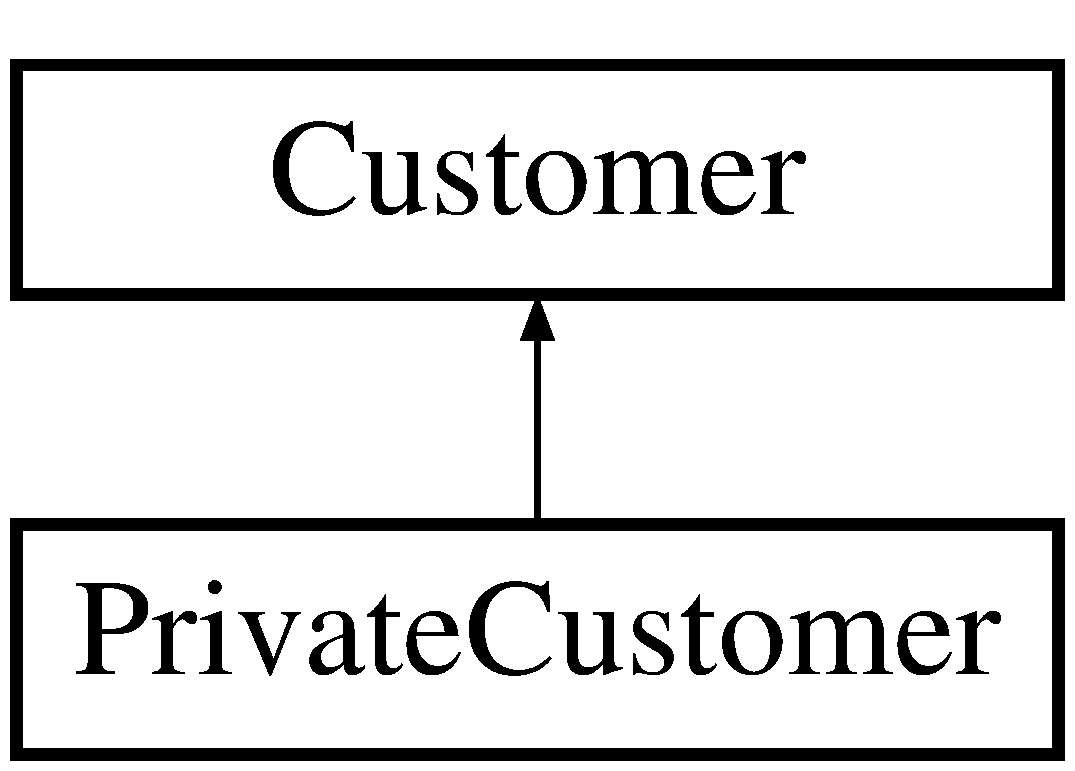
\includegraphics[height=2.000000cm]{classPrivateCustomer}
\end{center}
\end{figure}
\subsection*{Public Member Functions}
\begin{DoxyCompactItemize}
\item 
\hyperlink{classPrivateCustomer_ab9d59484ad8056c18e470d247d6c5fa6}{Private\+Customer} (unsigned int \hyperlink{classCustomer_a65ad3329532d5ad31e36f4ac81858e31}{nif}, string \hyperlink{classCustomer_a42c1c948fa0121c82b2725826d9f8300}{name}, string \hyperlink{classCustomer_a72d87951c1b76883390d00baf044cf2c}{address}, int \hyperlink{classCustomer_ad8c8d99b4c35f66a1a87b234c6078e0f}{phone\+Number}, int \hyperlink{classPrivateCustomer_a1dd69e30a5c32c3cab647f96eaa89325}{points})
\item 
\hyperlink{classPrivateCustomer_a916690ac1f0e8e28e9aeff4bb207169e}{$\sim$\+Private\+Customer} ()
\item 
int \hyperlink{classPrivateCustomer_ad8c8c1ff1cf54e6e60d73b7c6806e699}{get\+Points} ()
\item 
float \hyperlink{classPrivateCustomer_a4757f4e3cb5e0e74891e8f1b37a07277}{get\+Discount} ()
\item 
void \hyperlink{classPrivateCustomer_a22e7d589398c26ac37973660f6e6f338}{accumulate\+Service} (\hyperlink{classService}{Service} $\ast$service)
\item 
\hyperlink{classCustomer_adf157cb713398bb38163743659ec3049}{C\+U\+S\+T\+O\+M\+E\+R\+\_\+\+T\+Y\+PE} \hyperlink{classPrivateCustomer_a07d4d3e5995758b2407b8a81e35e579a}{get\+Customer\+Type} ()
\item 
string \hyperlink{classPrivateCustomer_afcf22c4a25e9c961d045aa5a0d8d9fd2}{get\+Information} ()
\item 
string \hyperlink{classPrivateCustomer_adb678cbc09d9e4a8e9e4ab0d556b8b6c}{to\+File\+Format} ()
\item 
void \hyperlink{classPrivateCustomer_a2e633d2d89e3ce4696e810ddb8c64bd0}{reset\+Points} ()
\end{DoxyCompactItemize}
\subsection*{Private Attributes}
\begin{DoxyCompactItemize}
\item 
int \hyperlink{classPrivateCustomer_a1dd69e30a5c32c3cab647f96eaa89325}{points}
\end{DoxyCompactItemize}
\subsection*{Additional Inherited Members}


\subsection{Constructor \& Destructor Documentation}
\hypertarget{classPrivateCustomer_ab9d59484ad8056c18e470d247d6c5fa6}{}\label{classPrivateCustomer_ab9d59484ad8056c18e470d247d6c5fa6} 
\index{Private\+Customer@{Private\+Customer}!Private\+Customer@{Private\+Customer}}
\index{Private\+Customer@{Private\+Customer}!Private\+Customer@{Private\+Customer}}
\subsubsection{\texorpdfstring{Private\+Customer()}{PrivateCustomer()}}
{\footnotesize\ttfamily Private\+Customer\+::\+Private\+Customer (\begin{DoxyParamCaption}\item[{unsigned int}]{nif,  }\item[{string}]{name,  }\item[{string}]{address,  }\item[{int}]{phone\+Number,  }\item[{int}]{points }\end{DoxyParamCaption})}

The constructor of the private customer class, where the elements are initialized. 
\begin{DoxyParams}{Parameters}
{\em nif} & customer nif \\
\hline
{\em name} & customer name \\
\hline
{\em address} & customer address \\
\hline
{\em phone\+Number} & customer phone number \\
\hline
{\em points} & customer points \\
\hline
\end{DoxyParams}
\hypertarget{classPrivateCustomer_a916690ac1f0e8e28e9aeff4bb207169e}{}\label{classPrivateCustomer_a916690ac1f0e8e28e9aeff4bb207169e} 
\index{Private\+Customer@{Private\+Customer}!````~Private\+Customer@{$\sim$\+Private\+Customer}}
\index{````~Private\+Customer@{$\sim$\+Private\+Customer}!Private\+Customer@{Private\+Customer}}
\subsubsection{\texorpdfstring{$\sim$\+Private\+Customer()}{~PrivateCustomer()}}
{\footnotesize\ttfamily Private\+Customer\+::$\sim$\+Private\+Customer (\begin{DoxyParamCaption}{ }\end{DoxyParamCaption})}

The destructor 

\subsection{Member Function Documentation}
\hypertarget{classPrivateCustomer_a22e7d589398c26ac37973660f6e6f338}{}\label{classPrivateCustomer_a22e7d589398c26ac37973660f6e6f338} 
\index{Private\+Customer@{Private\+Customer}!accumulate\+Service@{accumulate\+Service}}
\index{accumulate\+Service@{accumulate\+Service}!Private\+Customer@{Private\+Customer}}
\subsubsection{\texorpdfstring{accumulate\+Service()}{accumulateService()}}
{\footnotesize\ttfamily void Private\+Customer\+::accumulate\+Service (\begin{DoxyParamCaption}\item[{\hyperlink{classService}{Service} $\ast$}]{service }\end{DoxyParamCaption})\hspace{0.3cm}{\ttfamily [virtual]}}

Function that accumulate the service points. 
\begin{DoxyParams}{Parameters}
{\em service} & Private customer service \\
\hline
\end{DoxyParams}


Implements \hyperlink{classCustomer_ab42320f3e4d1c23e745ce901d30faf77}{Customer}.

\hypertarget{classPrivateCustomer_a07d4d3e5995758b2407b8a81e35e579a}{}\label{classPrivateCustomer_a07d4d3e5995758b2407b8a81e35e579a} 
\index{Private\+Customer@{Private\+Customer}!get\+Customer\+Type@{get\+Customer\+Type}}
\index{get\+Customer\+Type@{get\+Customer\+Type}!Private\+Customer@{Private\+Customer}}
\subsubsection{\texorpdfstring{get\+Customer\+Type()}{getCustomerType()}}
{\footnotesize\ttfamily \hyperlink{classCustomer_adf157cb713398bb38163743659ec3049}{Customer\+::\+C\+U\+S\+T\+O\+M\+E\+R\+\_\+\+T\+Y\+PE} Private\+Customer\+::get\+Customer\+Type (\begin{DoxyParamCaption}{ }\end{DoxyParamCaption})\hspace{0.3cm}{\ttfamily [virtual]}}

This \char`\"{}enumerator\char`\"{} type restricts the types of existing customers \begin{DoxyReturn}{Returns}
private customer 
\end{DoxyReturn}


Implements \hyperlink{classCustomer_a0353fcbdcb8ec729d95e9086df828e34}{Customer}.

\hypertarget{classPrivateCustomer_a4757f4e3cb5e0e74891e8f1b37a07277}{}\label{classPrivateCustomer_a4757f4e3cb5e0e74891e8f1b37a07277} 
\index{Private\+Customer@{Private\+Customer}!get\+Discount@{get\+Discount}}
\index{get\+Discount@{get\+Discount}!Private\+Customer@{Private\+Customer}}
\subsubsection{\texorpdfstring{get\+Discount()}{getDiscount()}}
{\footnotesize\ttfamily float Private\+Customer\+::get\+Discount (\begin{DoxyParamCaption}{ }\end{DoxyParamCaption})\hspace{0.3cm}{\ttfamily [virtual]}}

Function that through the points, get the discounts. If the points are less than 50, the customer doesn\textquotesingle{}t have discount. If the points are more than 50 and less than 100, the discount is 0,1 percent. If the points are more than 100 and less than 150, the discount is 0,2 percent. If the points are more than 150 and less than 200, the discount is 0,3 percent. If the points are more than 200 and less than 250, the discount is 0,4 percent. If the points are more than 250, the discount is 0,5 percent. \begin{DoxyReturn}{Returns}
the percent discount 
\end{DoxyReturn}


Implements \hyperlink{classCustomer_a55df4714c5be2c2978069eda6bc32ace}{Customer}.

\hypertarget{classPrivateCustomer_afcf22c4a25e9c961d045aa5a0d8d9fd2}{}\label{classPrivateCustomer_afcf22c4a25e9c961d045aa5a0d8d9fd2} 
\index{Private\+Customer@{Private\+Customer}!get\+Information@{get\+Information}}
\index{get\+Information@{get\+Information}!Private\+Customer@{Private\+Customer}}
\subsubsection{\texorpdfstring{get\+Information()}{getInformation()}}
{\footnotesize\ttfamily string Private\+Customer\+::get\+Information (\begin{DoxyParamCaption}{ }\end{DoxyParamCaption})\hspace{0.3cm}{\ttfamily [virtual]}}

Get a private customer information in line. \begin{DoxyReturn}{Returns}
a string with the customer information 
\end{DoxyReturn}


Reimplemented from \hyperlink{classCustomer_ae13da50be281b8f266f463a2166cad66}{Customer}.

\hypertarget{classPrivateCustomer_ad8c8c1ff1cf54e6e60d73b7c6806e699}{}\label{classPrivateCustomer_ad8c8c1ff1cf54e6e60d73b7c6806e699} 
\index{Private\+Customer@{Private\+Customer}!get\+Points@{get\+Points}}
\index{get\+Points@{get\+Points}!Private\+Customer@{Private\+Customer}}
\subsubsection{\texorpdfstring{get\+Points()}{getPoints()}}
{\footnotesize\ttfamily int Private\+Customer\+::get\+Points (\begin{DoxyParamCaption}{ }\end{DoxyParamCaption})}

Points is a private integer of the private customer class, we use \char`\"{}get\char`\"{} to be able to access this element in other classes. \hypertarget{classPrivateCustomer_a2e633d2d89e3ce4696e810ddb8c64bd0}{}\label{classPrivateCustomer_a2e633d2d89e3ce4696e810ddb8c64bd0} 
\index{Private\+Customer@{Private\+Customer}!reset\+Points@{reset\+Points}}
\index{reset\+Points@{reset\+Points}!Private\+Customer@{Private\+Customer}}
\subsubsection{\texorpdfstring{reset\+Points()}{resetPoints()}}
{\footnotesize\ttfamily void Private\+Customer\+::reset\+Points (\begin{DoxyParamCaption}{ }\end{DoxyParamCaption})}

Reset the customer points \hypertarget{classPrivateCustomer_adb678cbc09d9e4a8e9e4ab0d556b8b6c}{}\label{classPrivateCustomer_adb678cbc09d9e4a8e9e4ab0d556b8b6c} 
\index{Private\+Customer@{Private\+Customer}!to\+File\+Format@{to\+File\+Format}}
\index{to\+File\+Format@{to\+File\+Format}!Private\+Customer@{Private\+Customer}}
\subsubsection{\texorpdfstring{to\+File\+Format()}{toFileFormat()}}
{\footnotesize\ttfamily string Private\+Customer\+::to\+File\+Format (\begin{DoxyParamCaption}{ }\end{DoxyParamCaption})\hspace{0.3cm}{\ttfamily [virtual]}}

Returns a string with all information of the customer in the format needed. \begin{DoxyReturn}{Returns}
a string with the customer information in the format needed 
\end{DoxyReturn}


Reimplemented from \hyperlink{classCustomer_aa609cffee22046082003ea0ac3c191af}{Customer}.



\subsection{Member Data Documentation}
\hypertarget{classPrivateCustomer_a1dd69e30a5c32c3cab647f96eaa89325}{}\label{classPrivateCustomer_a1dd69e30a5c32c3cab647f96eaa89325} 
\index{Private\+Customer@{Private\+Customer}!points@{points}}
\index{points@{points}!Private\+Customer@{Private\+Customer}}
\subsubsection{\texorpdfstring{points}{points}}
{\footnotesize\ttfamily int Private\+Customer\+::points\hspace{0.3cm}{\ttfamily [private]}}



The documentation for this class was generated from the following files\+:\begin{DoxyCompactItemize}
\item 
src/\hyperlink{PrivateCustomer_8h}{Private\+Customer.\+h}\item 
src/\hyperlink{PrivateCustomer_8cpp}{Private\+Customer.\+cpp}\end{DoxyCompactItemize}

\hypertarget{classRoute}{}\section{Route Class Reference}
\label{classRoute}\index{Route@{Route}}


{\ttfamily \#include $<$Route.\+h$>$}

\subsection*{Public Member Functions}
\begin{DoxyCompactItemize}
\item 
\hyperlink{classRoute_a4b3c37aa39cb2fb44536b492bcd1f79e}{Route} (string \hyperlink{classRoute_a1534a1a4697d382624b37e9b8e18558c}{source}, string \hyperlink{classRoute_adc36330c18132468643c316cdcde3c86}{arrival}, double \hyperlink{classRoute_a8f6f506a1c61c2e27ba69e5eff5805a1}{distance}, int \hyperlink{classRoute_a1f2959ab7a51bd76846d649a7d93bdbe}{expected\+Time})
\item 
\hyperlink{classRoute_a946619c947f7a1a9d5303860c6a66005}{Route} (string \hyperlink{classRoute_a1534a1a4697d382624b37e9b8e18558c}{source}, string \hyperlink{classRoute_adc36330c18132468643c316cdcde3c86}{arrival})
\item 
\hyperlink{classRoute_a41212532f2bce3298d8f9468f82c62ab}{$\sim$\+Route} ()
\item 
string \hyperlink{classRoute_aded296bd92c4eadb9d2c64d2e5088220}{get\+Source} ()
\item 
string \hyperlink{classRoute_aaa88da20cc0c2f362f332288be26cd2c}{get\+Arrival} ()
\item 
double \hyperlink{classRoute_a4ccb609408c7d1e7020017b2de6e2f31}{get\+Distance} ()
\item 
int \hyperlink{classRoute_a5e9243c4341dee71d9f1c5a310b6538f}{get\+Expected\+Time} ()
\item 
string \hyperlink{classRoute_a7db106e71797ccd6eb91cf36fbe9987d}{get\+Expected\+Timein\+Format} ()
\item 
void \hyperlink{classRoute_ad39247fcbd404ef5755262e0c1cae04d}{set\+Source} (string \hyperlink{classRoute_a1534a1a4697d382624b37e9b8e18558c}{source})
\item 
void \hyperlink{classRoute_ad020607979b427d768f3c0f1f9600fb3}{set\+Arrival} (string \hyperlink{classRoute_adc36330c18132468643c316cdcde3c86}{arrival})
\item 
void \hyperlink{classRoute_a9bd5ad9f9bc229585f183a114c1709e1}{set\+Distance} (double \hyperlink{classRoute_a8f6f506a1c61c2e27ba69e5eff5805a1}{distance})
\item 
void \hyperlink{classRoute_a437920d776b005e425df9c5cfc5de450}{set\+Expected\+Time} (int \hyperlink{classRoute_a1f2959ab7a51bd76846d649a7d93bdbe}{expected\+Time})
\item 
string \hyperlink{classRoute_a3b912b298bc6c3c1656a2d31e6541315}{get\+Information} ()
\item 
string \hyperlink{classRoute_a2e6b5b3d06829495c0db27b63c9cf3a4}{to\+File\+Format} ()
\end{DoxyCompactItemize}
\subsection*{Private Attributes}
\begin{DoxyCompactItemize}
\item 
string \hyperlink{classRoute_a1534a1a4697d382624b37e9b8e18558c}{source}
\item 
string \hyperlink{classRoute_adc36330c18132468643c316cdcde3c86}{arrival}
\item 
double \hyperlink{classRoute_a8f6f506a1c61c2e27ba69e5eff5805a1}{distance}
\item 
int \hyperlink{classRoute_a1f2959ab7a51bd76846d649a7d93bdbe}{expected\+Time}
\end{DoxyCompactItemize}


\subsection{Constructor \& Destructor Documentation}
\hypertarget{classRoute_a4b3c37aa39cb2fb44536b492bcd1f79e}{}\label{classRoute_a4b3c37aa39cb2fb44536b492bcd1f79e} 
\index{Route@{Route}!Route@{Route}}
\index{Route@{Route}!Route@{Route}}
\subsubsection{\texorpdfstring{Route()}{Route()}\hspace{0.1cm}{\footnotesize\ttfamily [1/2]}}
{\footnotesize\ttfamily Route\+::\+Route (\begin{DoxyParamCaption}\item[{string}]{source,  }\item[{string}]{arrival,  }\item[{double}]{distance,  }\item[{int}]{expected\+Time }\end{DoxyParamCaption})}

The constructor of the \hyperlink{classRoute}{Route} class, where the elements are initialized. 
\begin{DoxyParams}{Parameters}
{\em source} & service source \\
\hline
{\em arrival} & service arrival \\
\hline
{\em distance} & route distance \\
\hline
{\em expected\+Time} & route expected time \\
\hline
\end{DoxyParams}
\hypertarget{classRoute_a946619c947f7a1a9d5303860c6a66005}{}\label{classRoute_a946619c947f7a1a9d5303860c6a66005} 
\index{Route@{Route}!Route@{Route}}
\index{Route@{Route}!Route@{Route}}
\subsubsection{\texorpdfstring{Route()}{Route()}\hspace{0.1cm}{\footnotesize\ttfamily [2/2]}}
{\footnotesize\ttfamily Route\+::\+Route (\begin{DoxyParamCaption}\item[{string}]{source,  }\item[{string}]{arrival }\end{DoxyParamCaption})}

The constructor of the \hyperlink{classRoute}{Route} class, where the elements are initialized. 
\begin{DoxyParams}{Parameters}
{\em source} & service source \\
\hline
{\em arrival} & service arrival \\
\hline
\end{DoxyParams}
\hypertarget{classRoute_a41212532f2bce3298d8f9468f82c62ab}{}\label{classRoute_a41212532f2bce3298d8f9468f82c62ab} 
\index{Route@{Route}!````~Route@{$\sim$\+Route}}
\index{````~Route@{$\sim$\+Route}!Route@{Route}}
\subsubsection{\texorpdfstring{$\sim$\+Route()}{~Route()}}
{\footnotesize\ttfamily Route\+::$\sim$\+Route (\begin{DoxyParamCaption}{ }\end{DoxyParamCaption})}

The destructor 

\subsection{Member Function Documentation}
\hypertarget{classRoute_aaa88da20cc0c2f362f332288be26cd2c}{}\label{classRoute_aaa88da20cc0c2f362f332288be26cd2c} 
\index{Route@{Route}!get\+Arrival@{get\+Arrival}}
\index{get\+Arrival@{get\+Arrival}!Route@{Route}}
\subsubsection{\texorpdfstring{get\+Arrival()}{getArrival()}}
{\footnotesize\ttfamily string Route\+::get\+Arrival (\begin{DoxyParamCaption}{ }\end{DoxyParamCaption})}

Arrival is a private string of the \hyperlink{classRoute}{Route} class, we use \char`\"{}get\char`\"{} to be able to access this element in other classes. \begin{DoxyReturn}{Returns}
route arrival 
\end{DoxyReturn}
\hypertarget{classRoute_a4ccb609408c7d1e7020017b2de6e2f31}{}\label{classRoute_a4ccb609408c7d1e7020017b2de6e2f31} 
\index{Route@{Route}!get\+Distance@{get\+Distance}}
\index{get\+Distance@{get\+Distance}!Route@{Route}}
\subsubsection{\texorpdfstring{get\+Distance()}{getDistance()}}
{\footnotesize\ttfamily double Route\+::get\+Distance (\begin{DoxyParamCaption}{ }\end{DoxyParamCaption})}

Distance is a private double of the \hyperlink{classRoute}{Route} class, we use \char`\"{}get\char`\"{} to be able to access this element in other classes. \begin{DoxyReturn}{Returns}
route distance 
\end{DoxyReturn}
\hypertarget{classRoute_a5e9243c4341dee71d9f1c5a310b6538f}{}\label{classRoute_a5e9243c4341dee71d9f1c5a310b6538f} 
\index{Route@{Route}!get\+Expected\+Time@{get\+Expected\+Time}}
\index{get\+Expected\+Time@{get\+Expected\+Time}!Route@{Route}}
\subsubsection{\texorpdfstring{get\+Expected\+Time()}{getExpectedTime()}}
{\footnotesize\ttfamily int Route\+::get\+Expected\+Time (\begin{DoxyParamCaption}{ }\end{DoxyParamCaption})}

Expected\+Time is a private integer of the \hyperlink{classRoute}{Route} class, we use \char`\"{}get\char`\"{} to be able to access this element in other classes. \begin{DoxyReturn}{Returns}
route expected time 
\end{DoxyReturn}
\hypertarget{classRoute_a7db106e71797ccd6eb91cf36fbe9987d}{}\label{classRoute_a7db106e71797ccd6eb91cf36fbe9987d} 
\index{Route@{Route}!get\+Expected\+Timein\+Format@{get\+Expected\+Timein\+Format}}
\index{get\+Expected\+Timein\+Format@{get\+Expected\+Timein\+Format}!Route@{Route}}
\subsubsection{\texorpdfstring{get\+Expected\+Timein\+Format()}{getExpectedTimeinFormat()}}
{\footnotesize\ttfamily string Route\+::get\+Expected\+Timein\+Format (\begin{DoxyParamCaption}{ }\end{DoxyParamCaption})}

Function that returns a string with the expected time of a route with the following format\+: \char`\"{}15h30m\char`\"{}. \begin{DoxyReturn}{Returns}
a string with the expected time in the formated needed 
\end{DoxyReturn}
\hypertarget{classRoute_a3b912b298bc6c3c1656a2d31e6541315}{}\label{classRoute_a3b912b298bc6c3c1656a2d31e6541315} 
\index{Route@{Route}!get\+Information@{get\+Information}}
\index{get\+Information@{get\+Information}!Route@{Route}}
\subsubsection{\texorpdfstring{get\+Information()}{getInformation()}}
{\footnotesize\ttfamily string Route\+::get\+Information (\begin{DoxyParamCaption}{ }\end{DoxyParamCaption})}

Get a route information in line with the routes table. \begin{DoxyReturn}{Returns}
a string with the route information 
\end{DoxyReturn}
\hypertarget{classRoute_aded296bd92c4eadb9d2c64d2e5088220}{}\label{classRoute_aded296bd92c4eadb9d2c64d2e5088220} 
\index{Route@{Route}!get\+Source@{get\+Source}}
\index{get\+Source@{get\+Source}!Route@{Route}}
\subsubsection{\texorpdfstring{get\+Source()}{getSource()}}
{\footnotesize\ttfamily string Route\+::get\+Source (\begin{DoxyParamCaption}{ }\end{DoxyParamCaption})}

Source is a private string of the \hyperlink{classRoute}{Route} class, we use \char`\"{}get\char`\"{} to be able to access this element in other classes. \begin{DoxyReturn}{Returns}
route source 
\end{DoxyReturn}
\hypertarget{classRoute_ad020607979b427d768f3c0f1f9600fb3}{}\label{classRoute_ad020607979b427d768f3c0f1f9600fb3} 
\index{Route@{Route}!set\+Arrival@{set\+Arrival}}
\index{set\+Arrival@{set\+Arrival}!Route@{Route}}
\subsubsection{\texorpdfstring{set\+Arrival()}{setArrival()}}
{\footnotesize\ttfamily void Route\+::set\+Arrival (\begin{DoxyParamCaption}\item[{string}]{arrival }\end{DoxyParamCaption})}

Set the route arrival 
\begin{DoxyParams}{Parameters}
{\em new} & route arrival \\
\hline
\end{DoxyParams}
\hypertarget{classRoute_a9bd5ad9f9bc229585f183a114c1709e1}{}\label{classRoute_a9bd5ad9f9bc229585f183a114c1709e1} 
\index{Route@{Route}!set\+Distance@{set\+Distance}}
\index{set\+Distance@{set\+Distance}!Route@{Route}}
\subsubsection{\texorpdfstring{set\+Distance()}{setDistance()}}
{\footnotesize\ttfamily void Route\+::set\+Distance (\begin{DoxyParamCaption}\item[{double}]{distance }\end{DoxyParamCaption})}

Set the route distance 
\begin{DoxyParams}{Parameters}
{\em new} & route distance \\
\hline
\end{DoxyParams}
\hypertarget{classRoute_a437920d776b005e425df9c5cfc5de450}{}\label{classRoute_a437920d776b005e425df9c5cfc5de450} 
\index{Route@{Route}!set\+Expected\+Time@{set\+Expected\+Time}}
\index{set\+Expected\+Time@{set\+Expected\+Time}!Route@{Route}}
\subsubsection{\texorpdfstring{set\+Expected\+Time()}{setExpectedTime()}}
{\footnotesize\ttfamily void Route\+::set\+Expected\+Time (\begin{DoxyParamCaption}\item[{int}]{expected\+Time }\end{DoxyParamCaption})}

Set the route expected time 
\begin{DoxyParams}{Parameters}
{\em new} & route expected time \\
\hline
\end{DoxyParams}
\hypertarget{classRoute_ad39247fcbd404ef5755262e0c1cae04d}{}\label{classRoute_ad39247fcbd404ef5755262e0c1cae04d} 
\index{Route@{Route}!set\+Source@{set\+Source}}
\index{set\+Source@{set\+Source}!Route@{Route}}
\subsubsection{\texorpdfstring{set\+Source()}{setSource()}}
{\footnotesize\ttfamily void Route\+::set\+Source (\begin{DoxyParamCaption}\item[{string}]{source }\end{DoxyParamCaption})}

Set the route source 
\begin{DoxyParams}{Parameters}
{\em new} & route source \\
\hline
\end{DoxyParams}
\hypertarget{classRoute_a2e6b5b3d06829495c0db27b63c9cf3a4}{}\label{classRoute_a2e6b5b3d06829495c0db27b63c9cf3a4} 
\index{Route@{Route}!to\+File\+Format@{to\+File\+Format}}
\index{to\+File\+Format@{to\+File\+Format}!Route@{Route}}
\subsubsection{\texorpdfstring{to\+File\+Format()}{toFileFormat()}}
{\footnotesize\ttfamily string Route\+::to\+File\+Format (\begin{DoxyParamCaption}{ }\end{DoxyParamCaption})}

Returns a string with all information of the route in the format needed. \begin{DoxyReturn}{Returns}
a string with the route information in the format needed 
\end{DoxyReturn}


\subsection{Member Data Documentation}
\hypertarget{classRoute_adc36330c18132468643c316cdcde3c86}{}\label{classRoute_adc36330c18132468643c316cdcde3c86} 
\index{Route@{Route}!arrival@{arrival}}
\index{arrival@{arrival}!Route@{Route}}
\subsubsection{\texorpdfstring{arrival}{arrival}}
{\footnotesize\ttfamily string Route\+::arrival\hspace{0.3cm}{\ttfamily [private]}}

\hypertarget{classRoute_a8f6f506a1c61c2e27ba69e5eff5805a1}{}\label{classRoute_a8f6f506a1c61c2e27ba69e5eff5805a1} 
\index{Route@{Route}!distance@{distance}}
\index{distance@{distance}!Route@{Route}}
\subsubsection{\texorpdfstring{distance}{distance}}
{\footnotesize\ttfamily double Route\+::distance\hspace{0.3cm}{\ttfamily [private]}}

\hypertarget{classRoute_a1f2959ab7a51bd76846d649a7d93bdbe}{}\label{classRoute_a1f2959ab7a51bd76846d649a7d93bdbe} 
\index{Route@{Route}!expected\+Time@{expected\+Time}}
\index{expected\+Time@{expected\+Time}!Route@{Route}}
\subsubsection{\texorpdfstring{expected\+Time}{expectedTime}}
{\footnotesize\ttfamily int Route\+::expected\+Time\hspace{0.3cm}{\ttfamily [private]}}

\hypertarget{classRoute_a1534a1a4697d382624b37e9b8e18558c}{}\label{classRoute_a1534a1a4697d382624b37e9b8e18558c} 
\index{Route@{Route}!source@{source}}
\index{source@{source}!Route@{Route}}
\subsubsection{\texorpdfstring{source}{source}}
{\footnotesize\ttfamily string Route\+::source\hspace{0.3cm}{\ttfamily [private]}}



The documentation for this class was generated from the following files\+:\begin{DoxyCompactItemize}
\item 
src/\hyperlink{Route_8h}{Route.\+h}\item 
src/\hyperlink{Route_8cpp}{Route.\+cpp}\end{DoxyCompactItemize}

\hypertarget{classService}{}\section{Service Class Reference}
\label{classService}\index{Service@{Service}}


{\ttfamily \#include $<$Service.\+h$>$}

\subsection*{Public Member Functions}
\begin{DoxyCompactItemize}
\item 
\hyperlink{classService_a95b72be1a13715eda67acd99698ca0b4}{Service} (\hyperlink{classCustomer}{Customer} $\ast$\hyperlink{classService_a1dbb66a7a35562c9f4b7f1654c286d75}{customer}, double \hyperlink{classService_a2ce3309e0dff48b5fe242512df62784b}{cost}, \hyperlink{classRoute}{Route} $\ast$\hyperlink{classService_a3059a95085ce11e13a69ff19bc919f9a}{route}, \hyperlink{classDate}{Date} \hyperlink{classService_a00e1fb44faf15d76b7633b888780baeb}{date}, int \hyperlink{classService_ad48b41e25edbf42e8f0a0314adc8de4e}{time}, string \hyperlink{classService_a832536bb266da871d50d14226bba3ac0}{payment})
\item 
\hyperlink{classService_af6c3577b59652ac817d1d76aaccee904}{$\sim$\+Service} ()
\item 
\hyperlink{classCustomer}{Customer} $\ast$ \hyperlink{classService_a8f1201be847de0e1209c6dbc6e31b169}{get\+Customer} ()
\item 
double \hyperlink{classService_aba6ad9ce7b18fd9b9317166d34e74332}{get\+Cost} ()
\item 
\hyperlink{classRoute}{Route} $\ast$ \hyperlink{classService_a5c8aedeb788fac846e5862f7c4af9853}{get\+Route} ()
\item 
\hyperlink{classDate}{Date} \hyperlink{classService_af0a4561b2506893b9026ca31afef179a}{get\+Date} ()
\item 
int \hyperlink{classService_a10995791b3188543e2f96c820717a17c}{get\+Time} ()
\item 
string \hyperlink{classService_aa0a732dc04ba4ec18709575f1dcdfee5}{get\+Timein\+Format} ()
\item 
\hyperlink{Service_8h_a484d0c1796736fcbe8a3a730617b663f}{P\+A\+Y\+M\+E\+N\+T\+\_\+\+T\+Y\+PE} \hyperlink{classService_a83ce29e76b859a6feb292f4f39661eaa}{get\+Payment} ()
\item 
string \hyperlink{classService_a8c484a24407d965fec9d9a292d58cefb}{get\+Information} ()
\item 
string \hyperlink{classService_a029d5a0362c6bca5cd6c8dd1c49f9f44}{get\+Payment\+As\+String} ()
\item 
string \hyperlink{classService_a4b8752741b37817a03bfc1e756174550}{to\+File\+Format} ()
\end{DoxyCompactItemize}
\subsection*{Static Public Attributes}
\begin{DoxyCompactItemize}
\item 
static double \hyperlink{classService_aee8dfc7647ae55570b8240b9dff699f4}{rate\+For\+Km} = 1.\+0
\item 
static double \hyperlink{classService_a6b98e1285e0eebbcddeab247336d0eb5}{rate\+For\+Extra\+Min} = 0.\+5
\end{DoxyCompactItemize}
\subsection*{Private Attributes}
\begin{DoxyCompactItemize}
\item 
\hyperlink{classCustomer}{Customer} $\ast$ \hyperlink{classService_a1dbb66a7a35562c9f4b7f1654c286d75}{customer}
\item 
double \hyperlink{classService_a2ce3309e0dff48b5fe242512df62784b}{cost}
\item 
\hyperlink{classRoute}{Route} $\ast$ \hyperlink{classService_a3059a95085ce11e13a69ff19bc919f9a}{route}
\item 
\hyperlink{classDate}{Date} \hyperlink{classService_a00e1fb44faf15d76b7633b888780baeb}{date}
\item 
int \hyperlink{classService_ad48b41e25edbf42e8f0a0314adc8de4e}{time}
\item 
\hyperlink{Service_8h_a484d0c1796736fcbe8a3a730617b663f}{P\+A\+Y\+M\+E\+N\+T\+\_\+\+T\+Y\+PE} \hyperlink{classService_a832536bb266da871d50d14226bba3ac0}{payment}
\end{DoxyCompactItemize}


\subsection{Constructor \& Destructor Documentation}
\hypertarget{classService_a95b72be1a13715eda67acd99698ca0b4}{}\label{classService_a95b72be1a13715eda67acd99698ca0b4} 
\index{Service@{Service}!Service@{Service}}
\index{Service@{Service}!Service@{Service}}
\subsubsection{\texorpdfstring{Service()}{Service()}}
{\footnotesize\ttfamily Service\+::\+Service (\begin{DoxyParamCaption}\item[{\hyperlink{classCustomer}{Customer} $\ast$}]{customer,  }\item[{double}]{cost,  }\item[{\hyperlink{classRoute}{Route} $\ast$}]{route,  }\item[{\hyperlink{classDate}{Date}}]{date,  }\item[{int}]{time,  }\item[{string}]{payment }\end{DoxyParamCaption})}

The constructor of the \hyperlink{classService}{Service} class, where the elements are initialized. 
\begin{DoxyParams}{Parameters}
{\em customer} & customer service \\
\hline
{\em cost} & total value of the services performed by the customer \\
\hline
{\em route} & service route \\
\hline
{\em date} & service date \\
\hline
{\em time} & duration of service \\
\hline
{\em payment} & service type of payment \\
\hline
\end{DoxyParams}
\hypertarget{classService_af6c3577b59652ac817d1d76aaccee904}{}\label{classService_af6c3577b59652ac817d1d76aaccee904} 
\index{Service@{Service}!````~Service@{$\sim$\+Service}}
\index{````~Service@{$\sim$\+Service}!Service@{Service}}
\subsubsection{\texorpdfstring{$\sim$\+Service()}{~Service()}}
{\footnotesize\ttfamily Service\+::$\sim$\+Service (\begin{DoxyParamCaption}{ }\end{DoxyParamCaption})}

The destructor 

\subsection{Member Function Documentation}
\hypertarget{classService_aba6ad9ce7b18fd9b9317166d34e74332}{}\label{classService_aba6ad9ce7b18fd9b9317166d34e74332} 
\index{Service@{Service}!get\+Cost@{get\+Cost}}
\index{get\+Cost@{get\+Cost}!Service@{Service}}
\subsubsection{\texorpdfstring{get\+Cost()}{getCost()}}
{\footnotesize\ttfamily double Service\+::get\+Cost (\begin{DoxyParamCaption}{ }\end{DoxyParamCaption})}

Cost is a private double of the \hyperlink{classService}{Service} class, we use \char`\"{}get\char`\"{} to be able to access this element in other classes. \begin{DoxyReturn}{Returns}
total value of the services performed by the customer 
\end{DoxyReturn}
\hypertarget{classService_a8f1201be847de0e1209c6dbc6e31b169}{}\label{classService_a8f1201be847de0e1209c6dbc6e31b169} 
\index{Service@{Service}!get\+Customer@{get\+Customer}}
\index{get\+Customer@{get\+Customer}!Service@{Service}}
\subsubsection{\texorpdfstring{get\+Customer()}{getCustomer()}}
{\footnotesize\ttfamily \hyperlink{classCustomer}{Customer} $\ast$ Service\+::get\+Customer (\begin{DoxyParamCaption}{ }\end{DoxyParamCaption})}

\hyperlink{classCustomer}{Customer} is a private customer of the \hyperlink{classService}{Service} class, we use \char`\"{}get\char`\"{} to be able to access this element in other classes. \begin{DoxyReturn}{Returns}
customer service 
\end{DoxyReturn}
\hypertarget{classService_af0a4561b2506893b9026ca31afef179a}{}\label{classService_af0a4561b2506893b9026ca31afef179a} 
\index{Service@{Service}!get\+Date@{get\+Date}}
\index{get\+Date@{get\+Date}!Service@{Service}}
\subsubsection{\texorpdfstring{get\+Date()}{getDate()}}
{\footnotesize\ttfamily \hyperlink{classDate}{Date} Service\+::get\+Date (\begin{DoxyParamCaption}{ }\end{DoxyParamCaption})}

\hyperlink{classDate}{Date} is a private date of the \hyperlink{classService}{Service} class, we use \char`\"{}get\char`\"{} to be able to access this element in other classes. \begin{DoxyReturn}{Returns}
service date 
\end{DoxyReturn}
\hypertarget{classService_a8c484a24407d965fec9d9a292d58cefb}{}\label{classService_a8c484a24407d965fec9d9a292d58cefb} 
\index{Service@{Service}!get\+Information@{get\+Information}}
\index{get\+Information@{get\+Information}!Service@{Service}}
\subsubsection{\texorpdfstring{get\+Information()}{getInformation()}}
{\footnotesize\ttfamily string Service\+::get\+Information (\begin{DoxyParamCaption}{ }\end{DoxyParamCaption})}

Get a service information in line with the services table. \begin{DoxyReturn}{Returns}
a string with the service information 
\end{DoxyReturn}
\hypertarget{classService_a83ce29e76b859a6feb292f4f39661eaa}{}\label{classService_a83ce29e76b859a6feb292f4f39661eaa} 
\index{Service@{Service}!get\+Payment@{get\+Payment}}
\index{get\+Payment@{get\+Payment}!Service@{Service}}
\subsubsection{\texorpdfstring{get\+Payment()}{getPayment()}}
{\footnotesize\ttfamily \hyperlink{Service_8h_a484d0c1796736fcbe8a3a730617b663f}{P\+A\+Y\+M\+E\+N\+T\+\_\+\+T\+Y\+PE} Service\+::get\+Payment (\begin{DoxyParamCaption}{ }\end{DoxyParamCaption})}

This \char`\"{}enumerator\char`\"{} type restricts existing payment types \begin{DoxyReturn}{Returns}
payment type 
\end{DoxyReturn}
\hypertarget{classService_a029d5a0362c6bca5cd6c8dd1c49f9f44}{}\label{classService_a029d5a0362c6bca5cd6c8dd1c49f9f44} 
\index{Service@{Service}!get\+Payment\+As\+String@{get\+Payment\+As\+String}}
\index{get\+Payment\+As\+String@{get\+Payment\+As\+String}!Service@{Service}}
\subsubsection{\texorpdfstring{get\+Payment\+As\+String()}{getPaymentAsString()}}
{\footnotesize\ttfamily string Service\+::get\+Payment\+As\+String (\begin{DoxyParamCaption}{ }\end{DoxyParamCaption})}

Get the payment as a string \begin{DoxyReturn}{Returns}
a string with the payment type 
\end{DoxyReturn}
\hypertarget{classService_a5c8aedeb788fac846e5862f7c4af9853}{}\label{classService_a5c8aedeb788fac846e5862f7c4af9853} 
\index{Service@{Service}!get\+Route@{get\+Route}}
\index{get\+Route@{get\+Route}!Service@{Service}}
\subsubsection{\texorpdfstring{get\+Route()}{getRoute()}}
{\footnotesize\ttfamily \hyperlink{classRoute}{Route} $\ast$ Service\+::get\+Route (\begin{DoxyParamCaption}{ }\end{DoxyParamCaption})}

\hyperlink{classRoute}{Route} is a private route of the \hyperlink{classService}{Service} class, we use \char`\"{}get\char`\"{} to be able to access this element in other classes. \begin{DoxyReturn}{Returns}
service route 
\end{DoxyReturn}
\hypertarget{classService_a10995791b3188543e2f96c820717a17c}{}\label{classService_a10995791b3188543e2f96c820717a17c} 
\index{Service@{Service}!get\+Time@{get\+Time}}
\index{get\+Time@{get\+Time}!Service@{Service}}
\subsubsection{\texorpdfstring{get\+Time()}{getTime()}}
{\footnotesize\ttfamily int Service\+::get\+Time (\begin{DoxyParamCaption}{ }\end{DoxyParamCaption})}

Time is a private integer of the \hyperlink{classService}{Service} class, we use \char`\"{}get\char`\"{} to be able to access this element in other classes. \begin{DoxyReturn}{Returns}
service time 
\end{DoxyReturn}
\hypertarget{classService_aa0a732dc04ba4ec18709575f1dcdfee5}{}\label{classService_aa0a732dc04ba4ec18709575f1dcdfee5} 
\index{Service@{Service}!get\+Timein\+Format@{get\+Timein\+Format}}
\index{get\+Timein\+Format@{get\+Timein\+Format}!Service@{Service}}
\subsubsection{\texorpdfstring{get\+Timein\+Format()}{getTimeinFormat()}}
{\footnotesize\ttfamily string Service\+::get\+Timein\+Format (\begin{DoxyParamCaption}{ }\end{DoxyParamCaption})}

Get the time with the following format\+: \char`\"{}15h30m\char`\"{}. \begin{DoxyReturn}{Returns}
a string with the time in the format needed 
\end{DoxyReturn}
\hypertarget{classService_a4b8752741b37817a03bfc1e756174550}{}\label{classService_a4b8752741b37817a03bfc1e756174550} 
\index{Service@{Service}!to\+File\+Format@{to\+File\+Format}}
\index{to\+File\+Format@{to\+File\+Format}!Service@{Service}}
\subsubsection{\texorpdfstring{to\+File\+Format()}{toFileFormat()}}
{\footnotesize\ttfamily string Service\+::to\+File\+Format (\begin{DoxyParamCaption}{ }\end{DoxyParamCaption})}

Put a service information in the format needed. \begin{DoxyReturn}{Returns}
a string with all information of the services in the format needed 
\end{DoxyReturn}


\subsection{Member Data Documentation}
\hypertarget{classService_a2ce3309e0dff48b5fe242512df62784b}{}\label{classService_a2ce3309e0dff48b5fe242512df62784b} 
\index{Service@{Service}!cost@{cost}}
\index{cost@{cost}!Service@{Service}}
\subsubsection{\texorpdfstring{cost}{cost}}
{\footnotesize\ttfamily double Service\+::cost\hspace{0.3cm}{\ttfamily [private]}}

\hypertarget{classService_a1dbb66a7a35562c9f4b7f1654c286d75}{}\label{classService_a1dbb66a7a35562c9f4b7f1654c286d75} 
\index{Service@{Service}!customer@{customer}}
\index{customer@{customer}!Service@{Service}}
\subsubsection{\texorpdfstring{customer}{customer}}
{\footnotesize\ttfamily \hyperlink{classCustomer}{Customer}$\ast$ Service\+::customer\hspace{0.3cm}{\ttfamily [private]}}

\hypertarget{classService_a00e1fb44faf15d76b7633b888780baeb}{}\label{classService_a00e1fb44faf15d76b7633b888780baeb} 
\index{Service@{Service}!date@{date}}
\index{date@{date}!Service@{Service}}
\subsubsection{\texorpdfstring{date}{date}}
{\footnotesize\ttfamily \hyperlink{classDate}{Date} Service\+::date\hspace{0.3cm}{\ttfamily [private]}}

\hypertarget{classService_a832536bb266da871d50d14226bba3ac0}{}\label{classService_a832536bb266da871d50d14226bba3ac0} 
\index{Service@{Service}!payment@{payment}}
\index{payment@{payment}!Service@{Service}}
\subsubsection{\texorpdfstring{payment}{payment}}
{\footnotesize\ttfamily \hyperlink{Service_8h_a484d0c1796736fcbe8a3a730617b663f}{P\+A\+Y\+M\+E\+N\+T\+\_\+\+T\+Y\+PE} Service\+::payment\hspace{0.3cm}{\ttfamily [private]}}

\hypertarget{classService_a6b98e1285e0eebbcddeab247336d0eb5}{}\label{classService_a6b98e1285e0eebbcddeab247336d0eb5} 
\index{Service@{Service}!rate\+For\+Extra\+Min@{rate\+For\+Extra\+Min}}
\index{rate\+For\+Extra\+Min@{rate\+For\+Extra\+Min}!Service@{Service}}
\subsubsection{\texorpdfstring{rate\+For\+Extra\+Min}{rateForExtraMin}}
{\footnotesize\ttfamily double Service\+::rate\+For\+Extra\+Min = 0.\+5\hspace{0.3cm}{\ttfamily [static]}}

\hypertarget{classService_aee8dfc7647ae55570b8240b9dff699f4}{}\label{classService_aee8dfc7647ae55570b8240b9dff699f4} 
\index{Service@{Service}!rate\+For\+Km@{rate\+For\+Km}}
\index{rate\+For\+Km@{rate\+For\+Km}!Service@{Service}}
\subsubsection{\texorpdfstring{rate\+For\+Km}{rateForKm}}
{\footnotesize\ttfamily double Service\+::rate\+For\+Km = 1.\+0\hspace{0.3cm}{\ttfamily [static]}}

\hypertarget{classService_a3059a95085ce11e13a69ff19bc919f9a}{}\label{classService_a3059a95085ce11e13a69ff19bc919f9a} 
\index{Service@{Service}!route@{route}}
\index{route@{route}!Service@{Service}}
\subsubsection{\texorpdfstring{route}{route}}
{\footnotesize\ttfamily \hyperlink{classRoute}{Route}$\ast$ Service\+::route\hspace{0.3cm}{\ttfamily [private]}}

\hypertarget{classService_ad48b41e25edbf42e8f0a0314adc8de4e}{}\label{classService_ad48b41e25edbf42e8f0a0314adc8de4e} 
\index{Service@{Service}!time@{time}}
\index{time@{time}!Service@{Service}}
\subsubsection{\texorpdfstring{time}{time}}
{\footnotesize\ttfamily int Service\+::time\hspace{0.3cm}{\ttfamily [private]}}



The documentation for this class was generated from the following files\+:\begin{DoxyCompactItemize}
\item 
src/\hyperlink{Service_8h}{Service.\+h}\item 
src/\hyperlink{Service_8cpp}{Service.\+cpp}\end{DoxyCompactItemize}

\hypertarget{classVoucher}{}\section{Voucher Class Reference}
\label{classVoucher}\index{Voucher@{Voucher}}


{\ttfamily \#include $<$Voucher.\+h$>$}

\subsection*{Public Member Functions}
\begin{DoxyCompactItemize}
\item 
\hyperlink{classVoucher_aec53b33fa78469b74a2a098d709d2628}{Voucher} (\hyperlink{classDate}{Date} \hyperlink{classVoucher_a68434d1be856aa11041f21bf9036b733}{duration}, double \hyperlink{classVoucher_a1a0c90ed8a1aac5c6a92cb1912a16572}{value})
\item 
void \hyperlink{classVoucher_a75ecfe9594cdbc6bcf6c38326672d040}{set\+Value} (double)
\item 
void \hyperlink{classVoucher_a1db87fd0a6b0ec16825c52a6f24fa4b1}{set\+Date} (\hyperlink{classDate}{Date})
\item 
\hyperlink{classDate}{Date} \hyperlink{classVoucher_a661d91c985c89f3cb9231db52c45a8f1}{get\+Duration} ()
\item 
double \hyperlink{classVoucher_a1fa7c64bf3bada3b425a05fd43311519}{get\+Value} ()
\item 
string \hyperlink{classVoucher_a3fbbf6a661b7542fa1012bb287d564d8}{get\+Information} ()
\item 
string \hyperlink{classVoucher_abac34093e355c27735b6e7bc04bae7bb}{to\+File\+Format} ()
\end{DoxyCompactItemize}
\subsection*{Private Attributes}
\begin{DoxyCompactItemize}
\item 
\hyperlink{classDate}{Date} \hyperlink{classVoucher_a68434d1be856aa11041f21bf9036b733}{duration}
\item 
double \hyperlink{classVoucher_a1a0c90ed8a1aac5c6a92cb1912a16572}{value}
\end{DoxyCompactItemize}


\subsection{Constructor \& Destructor Documentation}
\hypertarget{classVoucher_aec53b33fa78469b74a2a098d709d2628}{}\label{classVoucher_aec53b33fa78469b74a2a098d709d2628} 
\index{Voucher@{Voucher}!Voucher@{Voucher}}
\index{Voucher@{Voucher}!Voucher@{Voucher}}
\subsubsection{\texorpdfstring{Voucher()}{Voucher()}}
{\footnotesize\ttfamily Voucher\+::\+Voucher (\begin{DoxyParamCaption}\item[{\hyperlink{classDate}{Date}}]{duration,  }\item[{double}]{value }\end{DoxyParamCaption})}

The constructor of the \hyperlink{classVoucher}{Voucher} class, where the elements are initialized. 
\begin{DoxyParams}{Parameters}
{\em value} & voucher deadline \\
\hline
{\em value} & voucher value \\
\hline
\end{DoxyParams}


\subsection{Member Function Documentation}
\hypertarget{classVoucher_a661d91c985c89f3cb9231db52c45a8f1}{}\label{classVoucher_a661d91c985c89f3cb9231db52c45a8f1} 
\index{Voucher@{Voucher}!get\+Duration@{get\+Duration}}
\index{get\+Duration@{get\+Duration}!Voucher@{Voucher}}
\subsubsection{\texorpdfstring{get\+Duration()}{getDuration()}}
{\footnotesize\ttfamily \hyperlink{classDate}{Date} Voucher\+::get\+Duration (\begin{DoxyParamCaption}{ }\end{DoxyParamCaption})}

Duration is a private date of the \hyperlink{classVoucher}{Voucher} class, we use \char`\"{}get\char`\"{} to be able to access this element in other classes. \begin{DoxyReturn}{Returns}
voucher deadline 
\end{DoxyReturn}
\hypertarget{classVoucher_a3fbbf6a661b7542fa1012bb287d564d8}{}\label{classVoucher_a3fbbf6a661b7542fa1012bb287d564d8} 
\index{Voucher@{Voucher}!get\+Information@{get\+Information}}
\index{get\+Information@{get\+Information}!Voucher@{Voucher}}
\subsubsection{\texorpdfstring{get\+Information()}{getInformation()}}
{\footnotesize\ttfamily string Voucher\+::get\+Information (\begin{DoxyParamCaption}{ }\end{DoxyParamCaption})}

Get a voucher information. \begin{DoxyReturn}{Returns}
a string with the voucher information 
\end{DoxyReturn}
\hypertarget{classVoucher_a1fa7c64bf3bada3b425a05fd43311519}{}\label{classVoucher_a1fa7c64bf3bada3b425a05fd43311519} 
\index{Voucher@{Voucher}!get\+Value@{get\+Value}}
\index{get\+Value@{get\+Value}!Voucher@{Voucher}}
\subsubsection{\texorpdfstring{get\+Value()}{getValue()}}
{\footnotesize\ttfamily double Voucher\+::get\+Value (\begin{DoxyParamCaption}{ }\end{DoxyParamCaption})}

Value is a private double of the \hyperlink{classVoucher}{Voucher} class, we use \char`\"{}get\char`\"{} to be able to access this element in other classes. \begin{DoxyReturn}{Returns}
voucher value 
\end{DoxyReturn}
\hypertarget{classVoucher_a1db87fd0a6b0ec16825c52a6f24fa4b1}{}\label{classVoucher_a1db87fd0a6b0ec16825c52a6f24fa4b1} 
\index{Voucher@{Voucher}!set\+Date@{set\+Date}}
\index{set\+Date@{set\+Date}!Voucher@{Voucher}}
\subsubsection{\texorpdfstring{set\+Date()}{setDate()}}
{\footnotesize\ttfamily void Voucher\+::set\+Date (\begin{DoxyParamCaption}\item[{\hyperlink{classDate}{Date}}]{date }\end{DoxyParamCaption})}

Set the deadline voucher 
\begin{DoxyParams}{Parameters}
{\em date} & voucher date \\
\hline
\end{DoxyParams}
\hypertarget{classVoucher_a75ecfe9594cdbc6bcf6c38326672d040}{}\label{classVoucher_a75ecfe9594cdbc6bcf6c38326672d040} 
\index{Voucher@{Voucher}!set\+Value@{set\+Value}}
\index{set\+Value@{set\+Value}!Voucher@{Voucher}}
\subsubsection{\texorpdfstring{set\+Value()}{setValue()}}
{\footnotesize\ttfamily void Voucher\+::set\+Value (\begin{DoxyParamCaption}\item[{double}]{value }\end{DoxyParamCaption})}

Set a voucher value. 
\begin{DoxyParams}{Parameters}
{\em voucher} & value \\
\hline
\end{DoxyParams}
\hypertarget{classVoucher_abac34093e355c27735b6e7bc04bae7bb}{}\label{classVoucher_abac34093e355c27735b6e7bc04bae7bb} 
\index{Voucher@{Voucher}!to\+File\+Format@{to\+File\+Format}}
\index{to\+File\+Format@{to\+File\+Format}!Voucher@{Voucher}}
\subsubsection{\texorpdfstring{to\+File\+Format()}{toFileFormat()}}
{\footnotesize\ttfamily string Voucher\+::to\+File\+Format (\begin{DoxyParamCaption}{ }\end{DoxyParamCaption})}

Returns a string with all information of the voucher in the format needed. \begin{DoxyReturn}{Returns}
a string with the voucher information in the format needed 
\end{DoxyReturn}


\subsection{Member Data Documentation}
\hypertarget{classVoucher_a68434d1be856aa11041f21bf9036b733}{}\label{classVoucher_a68434d1be856aa11041f21bf9036b733} 
\index{Voucher@{Voucher}!duration@{duration}}
\index{duration@{duration}!Voucher@{Voucher}}
\subsubsection{\texorpdfstring{duration}{duration}}
{\footnotesize\ttfamily \hyperlink{classDate}{Date} Voucher\+::duration\hspace{0.3cm}{\ttfamily [private]}}

\hypertarget{classVoucher_a1a0c90ed8a1aac5c6a92cb1912a16572}{}\label{classVoucher_a1a0c90ed8a1aac5c6a92cb1912a16572} 
\index{Voucher@{Voucher}!value@{value}}
\index{value@{value}!Voucher@{Voucher}}
\subsubsection{\texorpdfstring{value}{value}}
{\footnotesize\ttfamily double Voucher\+::value\hspace{0.3cm}{\ttfamily [private]}}



The documentation for this class was generated from the following files\+:\begin{DoxyCompactItemize}
\item 
src/\hyperlink{Voucher_8h}{Voucher.\+h}\item 
src/\hyperlink{Voucher_8cpp}{Voucher.\+cpp}\end{DoxyCompactItemize}

\chapter{File Documentation}
\hypertarget{CentralTaxis_8cpp}{}\section{src/\+Central\+Taxis.cpp File Reference}
\label{CentralTaxis_8cpp}\index{src/\+Central\+Taxis.\+cpp@{src/\+Central\+Taxis.\+cpp}}
{\ttfamily \#include \char`\"{}Central\+Taxis.\+h\char`\"{}}\newline

\hypertarget{CentralTaxis_8h}{}\section{src/\+Central\+Taxis.h File Reference}
\label{CentralTaxis_8h}\index{src/\+Central\+Taxis.\+h@{src/\+Central\+Taxis.\+h}}
{\ttfamily \#include \char`\"{}Customer.\+h\char`\"{}}\newline
{\ttfamily \#include \char`\"{}Private\+Customer.\+h\char`\"{}}\newline
{\ttfamily \#include \char`\"{}Company\+Customer.\+h\char`\"{}}\newline
{\ttfamily \#include \char`\"{}Service.\+h\char`\"{}}\newline
{\ttfamily \#include \char`\"{}Route.\+h\char`\"{}}\newline
{\ttfamily \#include \char`\"{}Voucher.\+h\char`\"{}}\newline
{\ttfamily \#include \char`\"{}Date.\+h\char`\"{}}\newline
{\ttfamily \#include \char`\"{}utilities.\+h\char`\"{}}\newline
{\ttfamily \#include $<$vector$>$}\newline
{\ttfamily \#include $<$string$>$}\newline
{\ttfamily \#include $<$fstream$>$}\newline
{\ttfamily \#include $<$iostream$>$}\newline
{\ttfamily \#include $<$sstream$>$}\newline
{\ttfamily \#include $<$algorithm$>$}\newline
{\ttfamily \#include $<$utility$>$}\newline
{\ttfamily \#include $<$math.\+h$>$}\newline
{\ttfamily \#include $<$map$>$}\newline
\subsection*{Classes}
\begin{DoxyCompactItemize}
\item 
class \hyperlink{classCentralTaxis}{Central\+Taxis}
\end{DoxyCompactItemize}

\hypertarget{CompanyCustomer_8cpp}{}\section{src/\+Company\+Customer.cpp File Reference}
\label{CompanyCustomer_8cpp}\index{src/\+Company\+Customer.\+cpp@{src/\+Company\+Customer.\+cpp}}
{\ttfamily \#include \char`\"{}Company\+Customer.\+h\char`\"{}}\newline

\hypertarget{CompanyCustomer_8h}{}\section{src/\+Company\+Customer.h File Reference}
\label{CompanyCustomer_8h}\index{src/\+Company\+Customer.\+h@{src/\+Company\+Customer.\+h}}
{\ttfamily \#include \char`\"{}Customer.\+h\char`\"{}}\newline
{\ttfamily \#include \char`\"{}Service.\+h\char`\"{}}\newline
{\ttfamily \#include \char`\"{}Voucher.\+h\char`\"{}}\newline
{\ttfamily \#include $<$vector$>$}\newline
{\ttfamily \#include $<$string$>$}\newline
{\ttfamily \#include $<$sstream$>$}\newline
{\ttfamily \#include $<$iostream$>$}\newline
\subsection*{Classes}
\begin{DoxyCompactItemize}
\item 
class \hyperlink{classCompanyCustomer}{Company\+Customer}
\end{DoxyCompactItemize}

\hypertarget{Customer_8cpp}{}\section{src/\+Customer.cpp File Reference}
\label{Customer_8cpp}\index{src/\+Customer.\+cpp@{src/\+Customer.\+cpp}}
{\ttfamily \#include \char`\"{}Customer.\+h\char`\"{}}\newline
\subsection*{Functions}
\begin{DoxyCompactItemize}
\item 
unsigned int \hyperlink{Customer_8cpp_a6b303e551a85a66f41a88c2b0ea5619f}{read\+Customer\+Nif} ()
\item 
unsigned int \hyperlink{Customer_8cpp_a91935ab31bb88133a519dece13225c2d}{read\+Customer\+Phone\+Number} ()
\item 
bool \hyperlink{Customer_8cpp_a7eb95f72d44978124a93a2581cadf3d4}{compare\+By\+Name} (\hyperlink{classCustomer}{Customer} $\ast$name\+\_\+a, \hyperlink{classCustomer}{Customer} $\ast$name\+\_\+b)
\item 
bool \hyperlink{Customer_8cpp_aff13f62e3bc97fd5254daa68a4e5edaa}{compare\+By\+Nif} (\hyperlink{classCustomer}{Customer} $\ast$nif\+\_\+a, \hyperlink{classCustomer}{Customer} $\ast$nif\+\_\+b)
\item 
void \hyperlink{Customer_8cpp_a277b17dbda038647325432ce81544acb}{print\+Customer\+Table} ()
\item 
void \hyperlink{Customer_8cpp_a674a07a3017e41f980baf4be733a4cb5}{print\+Customer\+Table\+Type} (char type)
\item 
void \hyperlink{Customer_8cpp_aca416738432da9ffb09b06355ff98387}{show\+All\+Customers\+Info} (vector$<$ \hyperlink{classCustomer}{Customer} $\ast$$>$ customers)
\item 
void \hyperlink{Customer_8cpp_af873e620b4282f14fc35deb349be6774}{show\+All\+Customers\+Info\+By\+Type} (vector$<$ \hyperlink{classCustomer}{Customer} $\ast$$>$ customers, char type)
\item 
\hyperlink{classCustomer}{Customer} $\ast$ \hyperlink{Customer_8cpp_ade28623b01af60703a7add5a1b62b831}{customer\+Exists} (unsigned int nif, vector$<$ \hyperlink{classCustomer}{Customer} $\ast$$>$ customers)
\item 
bool \hyperlink{Customer_8cpp_aa152b797656f02ec2036447ecc89702e}{verify\+Nif\+Already\+Exist} (unsigned int nif, vector$<$ \hyperlink{classCustomer}{Customer} $\ast$$>$ customers)
\item 
void \hyperlink{Customer_8cpp_aa11b91db561974e3cd595c78b5352f35}{show\+Customers\+Info\+By\+Nif} (vector$<$ \hyperlink{classCustomer}{Customer} $\ast$$>$ customers)
\item 
void \hyperlink{Customer_8cpp_a735779d71d7d7d3936cd4334b8380004}{show\+Customers\+Info\+By\+Name} (vector$<$ \hyperlink{classCustomer}{Customer} $\ast$$>$ customers)
\end{DoxyCompactItemize}


\subsection{Function Documentation}
\hypertarget{Customer_8cpp_a7eb95f72d44978124a93a2581cadf3d4}{}\label{Customer_8cpp_a7eb95f72d44978124a93a2581cadf3d4} 
\index{Customer.\+cpp@{Customer.\+cpp}!compare\+By\+Name@{compare\+By\+Name}}
\index{compare\+By\+Name@{compare\+By\+Name}!Customer.\+cpp@{Customer.\+cpp}}
\subsubsection{\texorpdfstring{compare\+By\+Name()}{compareByName()}}
{\footnotesize\ttfamily bool compare\+By\+Name (\begin{DoxyParamCaption}\item[{\hyperlink{classCustomer}{Customer} $\ast$}]{name\+\_\+a,  }\item[{\hyperlink{classCustomer}{Customer} $\ast$}]{name\+\_\+b }\end{DoxyParamCaption})}

Function used while sorting customers by name. 
\begin{DoxyParams}{Parameters}
{\em name\+\_\+a} & first customer to compare \\
\hline
{\em name\+\_\+b} & second customer to compare \\
\hline
\end{DoxyParams}
\begin{DoxyReturn}{Returns}
if the name\+\_\+a is less than name\+\_\+b 
\end{DoxyReturn}
\hypertarget{Customer_8cpp_aff13f62e3bc97fd5254daa68a4e5edaa}{}\label{Customer_8cpp_aff13f62e3bc97fd5254daa68a4e5edaa} 
\index{Customer.\+cpp@{Customer.\+cpp}!compare\+By\+Nif@{compare\+By\+Nif}}
\index{compare\+By\+Nif@{compare\+By\+Nif}!Customer.\+cpp@{Customer.\+cpp}}
\subsubsection{\texorpdfstring{compare\+By\+Nif()}{compareByNif()}}
{\footnotesize\ttfamily bool compare\+By\+Nif (\begin{DoxyParamCaption}\item[{\hyperlink{classCustomer}{Customer} $\ast$}]{nif\+\_\+a,  }\item[{\hyperlink{classCustomer}{Customer} $\ast$}]{nif\+\_\+b }\end{DoxyParamCaption})}

Function used while sorting customers by nif. 
\begin{DoxyParams}{Parameters}
{\em nif\+\_\+a} & first customer to compare \\
\hline
{\em nif\+\_\+b} & second customer to compare \\
\hline
\end{DoxyParams}
\begin{DoxyReturn}{Returns}
if the nif\+\_\+a is less than nif\+\_\+b 
\end{DoxyReturn}
\hypertarget{Customer_8cpp_ade28623b01af60703a7add5a1b62b831}{}\label{Customer_8cpp_ade28623b01af60703a7add5a1b62b831} 
\index{Customer.\+cpp@{Customer.\+cpp}!customer\+Exists@{customer\+Exists}}
\index{customer\+Exists@{customer\+Exists}!Customer.\+cpp@{Customer.\+cpp}}
\subsubsection{\texorpdfstring{customer\+Exists()}{customerExists()}}
{\footnotesize\ttfamily \hyperlink{classCustomer}{Customer} $\ast$ customer\+Exists (\begin{DoxyParamCaption}\item[{unsigned int}]{nif,  }\item[{vector$<$ \hyperlink{classCustomer}{Customer} $\ast$$>$}]{customers }\end{DoxyParamCaption})}

Verify if the customer exists, if not return a null customer. 
\begin{DoxyParams}{Parameters}
{\em nif} & customer nif to look for \\
\hline
{\em customers} & customers vector \\
\hline
\end{DoxyParams}
\begin{DoxyReturn}{Returns}
the customer with the nif receive 
\end{DoxyReturn}
\hypertarget{Customer_8cpp_a277b17dbda038647325432ce81544acb}{}\label{Customer_8cpp_a277b17dbda038647325432ce81544acb} 
\index{Customer.\+cpp@{Customer.\+cpp}!print\+Customer\+Table@{print\+Customer\+Table}}
\index{print\+Customer\+Table@{print\+Customer\+Table}!Customer.\+cpp@{Customer.\+cpp}}
\subsubsection{\texorpdfstring{print\+Customer\+Table()}{printCustomerTable()}}
{\footnotesize\ttfamily void print\+Customer\+Table (\begin{DoxyParamCaption}{ }\end{DoxyParamCaption})}

Print the customer table. \hypertarget{Customer_8cpp_a674a07a3017e41f980baf4be733a4cb5}{}\label{Customer_8cpp_a674a07a3017e41f980baf4be733a4cb5} 
\index{Customer.\+cpp@{Customer.\+cpp}!print\+Customer\+Table\+Type@{print\+Customer\+Table\+Type}}
\index{print\+Customer\+Table\+Type@{print\+Customer\+Table\+Type}!Customer.\+cpp@{Customer.\+cpp}}
\subsubsection{\texorpdfstring{print\+Customer\+Table\+Type()}{printCustomerTableType()}}
{\footnotesize\ttfamily void print\+Customer\+Table\+Type (\begin{DoxyParamCaption}\item[{char}]{type }\end{DoxyParamCaption})}

Print the customer table type. 
\begin{DoxyParams}{Parameters}
{\em type} & customer type \\
\hline
\end{DoxyParams}
\hypertarget{Customer_8cpp_a6b303e551a85a66f41a88c2b0ea5619f}{}\label{Customer_8cpp_a6b303e551a85a66f41a88c2b0ea5619f} 
\index{Customer.\+cpp@{Customer.\+cpp}!read\+Customer\+Nif@{read\+Customer\+Nif}}
\index{read\+Customer\+Nif@{read\+Customer\+Nif}!Customer.\+cpp@{Customer.\+cpp}}
\subsubsection{\texorpdfstring{read\+Customer\+Nif()}{readCustomerNif()}}
{\footnotesize\ttfamily unsigned int read\+Customer\+Nif (\begin{DoxyParamCaption}{ }\end{DoxyParamCaption})}

Read the customer N\+IF. \begin{DoxyReturn}{Returns}
customer nif 
\end{DoxyReturn}

\begin{DoxyExceptions}{Exceptions}
{\em \hyperlink{classInvalidNifException}{Invalid\+Nif\+Exception}} & \\
\hline
\end{DoxyExceptions}
\hypertarget{Customer_8cpp_a91935ab31bb88133a519dece13225c2d}{}\label{Customer_8cpp_a91935ab31bb88133a519dece13225c2d} 
\index{Customer.\+cpp@{Customer.\+cpp}!read\+Customer\+Phone\+Number@{read\+Customer\+Phone\+Number}}
\index{read\+Customer\+Phone\+Number@{read\+Customer\+Phone\+Number}!Customer.\+cpp@{Customer.\+cpp}}
\subsubsection{\texorpdfstring{read\+Customer\+Phone\+Number()}{readCustomerPhoneNumber()}}
{\footnotesize\ttfamily unsigned int read\+Customer\+Phone\+Number (\begin{DoxyParamCaption}{ }\end{DoxyParamCaption})}

Read the customer phone number. \begin{DoxyReturn}{Returns}
customer phone number 
\end{DoxyReturn}

\begin{DoxyExceptions}{Exceptions}
{\em \hyperlink{classInvalidPhoneNumberException}{Invalid\+Phone\+Number\+Exception}} & \\
\hline
\end{DoxyExceptions}
\hypertarget{Customer_8cpp_aca416738432da9ffb09b06355ff98387}{}\label{Customer_8cpp_aca416738432da9ffb09b06355ff98387} 
\index{Customer.\+cpp@{Customer.\+cpp}!show\+All\+Customers\+Info@{show\+All\+Customers\+Info}}
\index{show\+All\+Customers\+Info@{show\+All\+Customers\+Info}!Customer.\+cpp@{Customer.\+cpp}}
\subsubsection{\texorpdfstring{show\+All\+Customers\+Info()}{showAllCustomersInfo()}}
{\footnotesize\ttfamily void show\+All\+Customers\+Info (\begin{DoxyParamCaption}\item[{vector$<$ \hyperlink{classCustomer}{Customer} $\ast$$>$}]{customers }\end{DoxyParamCaption})}

Show all the customer information in line with the customer table. 
\begin{DoxyParams}{Parameters}
{\em customers} & vector of customers \\
\hline
\end{DoxyParams}
\hypertarget{Customer_8cpp_af873e620b4282f14fc35deb349be6774}{}\label{Customer_8cpp_af873e620b4282f14fc35deb349be6774} 
\index{Customer.\+cpp@{Customer.\+cpp}!show\+All\+Customers\+Info\+By\+Type@{show\+All\+Customers\+Info\+By\+Type}}
\index{show\+All\+Customers\+Info\+By\+Type@{show\+All\+Customers\+Info\+By\+Type}!Customer.\+cpp@{Customer.\+cpp}}
\subsubsection{\texorpdfstring{show\+All\+Customers\+Info\+By\+Type()}{showAllCustomersInfoByType()}}
{\footnotesize\ttfamily void show\+All\+Customers\+Info\+By\+Type (\begin{DoxyParamCaption}\item[{vector$<$ \hyperlink{classCustomer}{Customer} $\ast$$>$}]{customers,  }\item[{char}]{type }\end{DoxyParamCaption})}

Show all the customer information by customer type in line with the customer table. 
\begin{DoxyParams}{Parameters}
{\em customers} & vector of customers \\
\hline
{\em type} & customer type \\
\hline
\end{DoxyParams}
\hypertarget{Customer_8cpp_a735779d71d7d7d3936cd4334b8380004}{}\label{Customer_8cpp_a735779d71d7d7d3936cd4334b8380004} 
\index{Customer.\+cpp@{Customer.\+cpp}!show\+Customers\+Info\+By\+Name@{show\+Customers\+Info\+By\+Name}}
\index{show\+Customers\+Info\+By\+Name@{show\+Customers\+Info\+By\+Name}!Customer.\+cpp@{Customer.\+cpp}}
\subsubsection{\texorpdfstring{show\+Customers\+Info\+By\+Name()}{showCustomersInfoByName()}}
{\footnotesize\ttfamily void show\+Customers\+Info\+By\+Name (\begin{DoxyParamCaption}\item[{vector$<$ \hyperlink{classCustomer}{Customer} $\ast$$>$}]{customers }\end{DoxyParamCaption})}

Shows the information of one customer, who is searched by the name. 
\begin{DoxyParams}{Parameters}
{\em customers} & customers vector \\
\hline
\end{DoxyParams}
\hypertarget{Customer_8cpp_aa11b91db561974e3cd595c78b5352f35}{}\label{Customer_8cpp_aa11b91db561974e3cd595c78b5352f35} 
\index{Customer.\+cpp@{Customer.\+cpp}!show\+Customers\+Info\+By\+Nif@{show\+Customers\+Info\+By\+Nif}}
\index{show\+Customers\+Info\+By\+Nif@{show\+Customers\+Info\+By\+Nif}!Customer.\+cpp@{Customer.\+cpp}}
\subsubsection{\texorpdfstring{show\+Customers\+Info\+By\+Nif()}{showCustomersInfoByNif()}}
{\footnotesize\ttfamily void show\+Customers\+Info\+By\+Nif (\begin{DoxyParamCaption}\item[{vector$<$ \hyperlink{classCustomer}{Customer} $\ast$$>$}]{customers }\end{DoxyParamCaption})}

Shows the information of one customer, who is searched by the N\+IF. 
\begin{DoxyParams}{Parameters}
{\em customers} & customers vector \\
\hline
\end{DoxyParams}
\hypertarget{Customer_8cpp_aa152b797656f02ec2036447ecc89702e}{}\label{Customer_8cpp_aa152b797656f02ec2036447ecc89702e} 
\index{Customer.\+cpp@{Customer.\+cpp}!verify\+Nif\+Already\+Exist@{verify\+Nif\+Already\+Exist}}
\index{verify\+Nif\+Already\+Exist@{verify\+Nif\+Already\+Exist}!Customer.\+cpp@{Customer.\+cpp}}
\subsubsection{\texorpdfstring{verify\+Nif\+Already\+Exist()}{verifyNifAlreadyExist()}}
{\footnotesize\ttfamily bool verify\+Nif\+Already\+Exist (\begin{DoxyParamCaption}\item[{unsigned int}]{nif,  }\item[{vector$<$ \hyperlink{classCustomer}{Customer} $\ast$$>$}]{customers }\end{DoxyParamCaption})}

Verify if the customer nif already exists 
\hypertarget{Customer_8h}{}\section{src/\+Customer.h File Reference}
\label{Customer_8h}\index{src/\+Customer.\+h@{src/\+Customer.\+h}}
{\ttfamily \#include \char`\"{}Service.\+h\char`\"{}}\newline
{\ttfamily \#include $<$vector$>$}\newline
{\ttfamily \#include $<$string$>$}\newline
{\ttfamily \#include $<$iostream$>$}\newline
{\ttfamily \#include $<$iomanip$>$}\newline
{\ttfamily \#include $<$algorithm$>$}\newline
{\ttfamily \#include $<$sstream$>$}\newline
{\ttfamily \#include $<$utility$>$}\newline
\subsection*{Classes}
\begin{DoxyCompactItemize}
\item 
class \hyperlink{classCustomer}{Customer}
\item 
class \hyperlink{classInvalidNifException}{Invalid\+Nif\+Exception}
\item 
class \hyperlink{classInvalidPhoneNumberException}{Invalid\+Phone\+Number\+Exception}
\end{DoxyCompactItemize}
\subsection*{Functions}
\begin{DoxyCompactItemize}
\item 
unsigned int \hyperlink{Customer_8h_a6b303e551a85a66f41a88c2b0ea5619f}{read\+Customer\+Nif} ()
\item 
\hyperlink{classCustomer}{Customer} $\ast$ \hyperlink{Customer_8h_a3c808b66a421907992cb79b6b7398351}{customer\+Exists} (unsigned int, vector$<$ \hyperlink{classCustomer}{Customer} $\ast$$>$)
\item 
unsigned int \hyperlink{Customer_8h_a91935ab31bb88133a519dece13225c2d}{read\+Customer\+Phone\+Number} ()
\item 
bool \hyperlink{Customer_8h_ab41a9ba811bbe9fd5ec4f653b85efb24}{verify\+Nif\+Already\+Exist} (unsigned int, vector$<$ \hyperlink{classCustomer}{Customer} $\ast$$>$)
\item 
bool \hyperlink{Customer_8h_ae7029443c3d6f9bfc3ef4fd285b07f5c}{compare\+By\+Nif} (\hyperlink{classCustomer}{Customer} $\ast$, \hyperlink{classCustomer}{Customer} $\ast$)
\item 
void \hyperlink{Customer_8h_a20da7e9e665cea14c6867c87097b9dea}{show\+All\+Customers\+Info} (vector$<$ \hyperlink{classCustomer}{Customer} $\ast$$>$)
\item 
void \hyperlink{Customer_8h_afe66cd0ba34a130a4cf152ae8dc5b388}{show\+Customers\+Info\+By\+Nif} (vector$<$ \hyperlink{classCustomer}{Customer} $\ast$$>$)
\item 
void \hyperlink{Customer_8h_a6a4ff1c26ad99c7c874391eb2d8b3673}{show\+Customers\+Info\+By\+Name} (vector$<$ \hyperlink{classCustomer}{Customer} $\ast$$>$)
\item 
void \hyperlink{Customer_8h_af873e620b4282f14fc35deb349be6774}{show\+All\+Customers\+Info\+By\+Type} (vector$<$ \hyperlink{classCustomer}{Customer} $\ast$$>$ customers, char type)
\end{DoxyCompactItemize}


\subsection{Function Documentation}
\hypertarget{Customer_8h_ae7029443c3d6f9bfc3ef4fd285b07f5c}{}\label{Customer_8h_ae7029443c3d6f9bfc3ef4fd285b07f5c} 
\index{Customer.\+h@{Customer.\+h}!compare\+By\+Nif@{compare\+By\+Nif}}
\index{compare\+By\+Nif@{compare\+By\+Nif}!Customer.\+h@{Customer.\+h}}
\subsubsection{\texorpdfstring{compare\+By\+Nif()}{compareByNif()}}
{\footnotesize\ttfamily bool compare\+By\+Nif (\begin{DoxyParamCaption}\item[{\hyperlink{classCustomer}{Customer} $\ast$}]{nif\+\_\+a,  }\item[{\hyperlink{classCustomer}{Customer} $\ast$}]{nif\+\_\+b }\end{DoxyParamCaption})}

Function used while sorting customers by nif. 
\begin{DoxyParams}{Parameters}
{\em nif\+\_\+a} & first customer to compare \\
\hline
{\em nif\+\_\+b} & second customer to compare \\
\hline
\end{DoxyParams}
\begin{DoxyReturn}{Returns}
if the nif\+\_\+a is less than nif\+\_\+b 
\end{DoxyReturn}
\hypertarget{Customer_8h_a3c808b66a421907992cb79b6b7398351}{}\label{Customer_8h_a3c808b66a421907992cb79b6b7398351} 
\index{Customer.\+h@{Customer.\+h}!customer\+Exists@{customer\+Exists}}
\index{customer\+Exists@{customer\+Exists}!Customer.\+h@{Customer.\+h}}
\subsubsection{\texorpdfstring{customer\+Exists()}{customerExists()}}
{\footnotesize\ttfamily \hyperlink{classCustomer}{Customer}$\ast$ customer\+Exists (\begin{DoxyParamCaption}\item[{unsigned}]{int,  }\item[{vector$<$ \hyperlink{classCustomer}{Customer} $\ast$$>$}]{ }\end{DoxyParamCaption})}

Verify if the customer exists, if not return a null customer. 
\begin{DoxyParams}{Parameters}
{\em nif} & customer nif to look for \\
\hline
{\em customers} & customers vector \\
\hline
\end{DoxyParams}
\begin{DoxyReturn}{Returns}
the customer with the nif receive 
\end{DoxyReturn}
\hypertarget{Customer_8h_a6b303e551a85a66f41a88c2b0ea5619f}{}\label{Customer_8h_a6b303e551a85a66f41a88c2b0ea5619f} 
\index{Customer.\+h@{Customer.\+h}!read\+Customer\+Nif@{read\+Customer\+Nif}}
\index{read\+Customer\+Nif@{read\+Customer\+Nif}!Customer.\+h@{Customer.\+h}}
\subsubsection{\texorpdfstring{read\+Customer\+Nif()}{readCustomerNif()}}
{\footnotesize\ttfamily unsigned int read\+Customer\+Nif (\begin{DoxyParamCaption}{ }\end{DoxyParamCaption})}

Read the customer N\+IF. \begin{DoxyReturn}{Returns}
customer nif 
\end{DoxyReturn}

\begin{DoxyExceptions}{Exceptions}
{\em \hyperlink{classInvalidNifException}{Invalid\+Nif\+Exception}} & \\
\hline
\end{DoxyExceptions}
\hypertarget{Customer_8h_a91935ab31bb88133a519dece13225c2d}{}\label{Customer_8h_a91935ab31bb88133a519dece13225c2d} 
\index{Customer.\+h@{Customer.\+h}!read\+Customer\+Phone\+Number@{read\+Customer\+Phone\+Number}}
\index{read\+Customer\+Phone\+Number@{read\+Customer\+Phone\+Number}!Customer.\+h@{Customer.\+h}}
\subsubsection{\texorpdfstring{read\+Customer\+Phone\+Number()}{readCustomerPhoneNumber()}}
{\footnotesize\ttfamily unsigned int read\+Customer\+Phone\+Number (\begin{DoxyParamCaption}{ }\end{DoxyParamCaption})}

Read the customer phone number. \begin{DoxyReturn}{Returns}
customer phone number 
\end{DoxyReturn}

\begin{DoxyExceptions}{Exceptions}
{\em \hyperlink{classInvalidPhoneNumberException}{Invalid\+Phone\+Number\+Exception}} & \\
\hline
\end{DoxyExceptions}
\hypertarget{Customer_8h_a20da7e9e665cea14c6867c87097b9dea}{}\label{Customer_8h_a20da7e9e665cea14c6867c87097b9dea} 
\index{Customer.\+h@{Customer.\+h}!show\+All\+Customers\+Info@{show\+All\+Customers\+Info}}
\index{show\+All\+Customers\+Info@{show\+All\+Customers\+Info}!Customer.\+h@{Customer.\+h}}
\subsubsection{\texorpdfstring{show\+All\+Customers\+Info()}{showAllCustomersInfo()}}
{\footnotesize\ttfamily void show\+All\+Customers\+Info (\begin{DoxyParamCaption}\item[{vector$<$ \hyperlink{classCustomer}{Customer} $\ast$$>$}]{customers }\end{DoxyParamCaption})}

Show all the customer information in line with the customer table. 
\begin{DoxyParams}{Parameters}
{\em customers} & vector of customers \\
\hline
\end{DoxyParams}
\hypertarget{Customer_8h_af873e620b4282f14fc35deb349be6774}{}\label{Customer_8h_af873e620b4282f14fc35deb349be6774} 
\index{Customer.\+h@{Customer.\+h}!show\+All\+Customers\+Info\+By\+Type@{show\+All\+Customers\+Info\+By\+Type}}
\index{show\+All\+Customers\+Info\+By\+Type@{show\+All\+Customers\+Info\+By\+Type}!Customer.\+h@{Customer.\+h}}
\subsubsection{\texorpdfstring{show\+All\+Customers\+Info\+By\+Type()}{showAllCustomersInfoByType()}}
{\footnotesize\ttfamily void show\+All\+Customers\+Info\+By\+Type (\begin{DoxyParamCaption}\item[{vector$<$ \hyperlink{classCustomer}{Customer} $\ast$$>$}]{customers,  }\item[{char}]{type }\end{DoxyParamCaption})}

Show all the customer information by customer type in line with the customer table. 
\begin{DoxyParams}{Parameters}
{\em customers} & vector of customers \\
\hline
{\em type} & customer type \\
\hline
\end{DoxyParams}
\hypertarget{Customer_8h_a6a4ff1c26ad99c7c874391eb2d8b3673}{}\label{Customer_8h_a6a4ff1c26ad99c7c874391eb2d8b3673} 
\index{Customer.\+h@{Customer.\+h}!show\+Customers\+Info\+By\+Name@{show\+Customers\+Info\+By\+Name}}
\index{show\+Customers\+Info\+By\+Name@{show\+Customers\+Info\+By\+Name}!Customer.\+h@{Customer.\+h}}
\subsubsection{\texorpdfstring{show\+Customers\+Info\+By\+Name()}{showCustomersInfoByName()}}
{\footnotesize\ttfamily void show\+Customers\+Info\+By\+Name (\begin{DoxyParamCaption}\item[{vector$<$ \hyperlink{classCustomer}{Customer} $\ast$$>$}]{customers }\end{DoxyParamCaption})}

Shows the information of one customer, who is searched by the name. 
\begin{DoxyParams}{Parameters}
{\em customers} & customers vector \\
\hline
\end{DoxyParams}
\hypertarget{Customer_8h_afe66cd0ba34a130a4cf152ae8dc5b388}{}\label{Customer_8h_afe66cd0ba34a130a4cf152ae8dc5b388} 
\index{Customer.\+h@{Customer.\+h}!show\+Customers\+Info\+By\+Nif@{show\+Customers\+Info\+By\+Nif}}
\index{show\+Customers\+Info\+By\+Nif@{show\+Customers\+Info\+By\+Nif}!Customer.\+h@{Customer.\+h}}
\subsubsection{\texorpdfstring{show\+Customers\+Info\+By\+Nif()}{showCustomersInfoByNif()}}
{\footnotesize\ttfamily void show\+Customers\+Info\+By\+Nif (\begin{DoxyParamCaption}\item[{vector$<$ \hyperlink{classCustomer}{Customer} $\ast$$>$}]{customers }\end{DoxyParamCaption})}

Shows the information of one customer, who is searched by the N\+IF. 
\begin{DoxyParams}{Parameters}
{\em customers} & customers vector \\
\hline
\end{DoxyParams}
\hypertarget{Customer_8h_ab41a9ba811bbe9fd5ec4f653b85efb24}{}\label{Customer_8h_ab41a9ba811bbe9fd5ec4f653b85efb24} 
\index{Customer.\+h@{Customer.\+h}!verify\+Nif\+Already\+Exist@{verify\+Nif\+Already\+Exist}}
\index{verify\+Nif\+Already\+Exist@{verify\+Nif\+Already\+Exist}!Customer.\+h@{Customer.\+h}}
\subsubsection{\texorpdfstring{verify\+Nif\+Already\+Exist()}{verifyNifAlreadyExist()}}
{\footnotesize\ttfamily bool verify\+Nif\+Already\+Exist (\begin{DoxyParamCaption}\item[{unsigned int}]{nif,  }\item[{vector$<$ \hyperlink{classCustomer}{Customer} $\ast$$>$}]{customers }\end{DoxyParamCaption})}

Verify if the customer nif already exists 
\hypertarget{Date_8cpp}{}\section{src/\+Date.cpp File Reference}
\label{Date_8cpp}\index{src/\+Date.\+cpp@{src/\+Date.\+cpp}}
{\ttfamily \#include $<$iostream$>$}\newline
{\ttfamily \#include $<$string$>$}\newline
{\ttfamily \#include $<$sstream$>$}\newline
{\ttfamily \#include $<$stdio.\+h$>$}\newline
{\ttfamily \#include $<$ctime$>$}\newline
{\ttfamily \#include \char`\"{}Date.\+h\char`\"{}}\newline
\subsection*{Functions}
\begin{DoxyCompactItemize}
\item 
string \hyperlink{Date_8cpp_a282294dcfdfd4992b27c7681fc05499a}{real\+Time} ()
\end{DoxyCompactItemize}


\subsection{Function Documentation}
\hypertarget{Date_8cpp_a282294dcfdfd4992b27c7681fc05499a}{}\label{Date_8cpp_a282294dcfdfd4992b27c7681fc05499a} 
\index{Date.\+cpp@{Date.\+cpp}!real\+Time@{real\+Time}}
\index{real\+Time@{real\+Time}!Date.\+cpp@{Date.\+cpp}}
\subsubsection{\texorpdfstring{real\+Time()}{realTime()}}
{\footnotesize\ttfamily string real\+Time (\begin{DoxyParamCaption}{ }\end{DoxyParamCaption})}

Function that returns the system date. \begin{DoxyReturn}{Returns}
a string with the system date 
\end{DoxyReturn}

\hypertarget{Date_8h}{}\section{src/\+Date.h File Reference}
\label{Date_8h}\index{src/\+Date.\+h@{src/\+Date.\+h}}
{\ttfamily \#include $<$iostream$>$}\newline
{\ttfamily \#include $<$string$>$}\newline
\subsection*{Classes}
\begin{DoxyCompactItemize}
\item 
class \hyperlink{classDate}{Date}
\end{DoxyCompactItemize}
\subsection*{Functions}
\begin{DoxyCompactItemize}
\item 
string \hyperlink{Date_8h_a282294dcfdfd4992b27c7681fc05499a}{real\+Time} ()
\end{DoxyCompactItemize}


\subsection{Function Documentation}
\hypertarget{Date_8h_a282294dcfdfd4992b27c7681fc05499a}{}\label{Date_8h_a282294dcfdfd4992b27c7681fc05499a} 
\index{Date.\+h@{Date.\+h}!real\+Time@{real\+Time}}
\index{real\+Time@{real\+Time}!Date.\+h@{Date.\+h}}
\subsubsection{\texorpdfstring{real\+Time()}{realTime()}}
{\footnotesize\ttfamily string real\+Time (\begin{DoxyParamCaption}{ }\end{DoxyParamCaption})}

Function that returns the system date. \begin{DoxyReturn}{Returns}
a string with the system date 
\end{DoxyReturn}

\hypertarget{main_8cpp}{}\section{src/main.cpp File Reference}
\label{main_8cpp}\index{src/main.\+cpp@{src/main.\+cpp}}
{\ttfamily \#include \char`\"{}Menu.\+h\char`\"{}}\newline
{\ttfamily \#include \char`\"{}Central\+Taxis.\+h\char`\"{}}\newline
{\ttfamily \#include $<$iostream$>$}\newline
{\ttfamily \#include $<$iomanip$>$}\newline
\subsection*{Functions}
\begin{DoxyCompactItemize}
\item 
int \hyperlink{main_8cpp_ae66f6b31b5ad750f1fe042a706a4e3d4}{main} ()
\end{DoxyCompactItemize}


\subsection{Function Documentation}
\hypertarget{main_8cpp_ae66f6b31b5ad750f1fe042a706a4e3d4}{}\label{main_8cpp_ae66f6b31b5ad750f1fe042a706a4e3d4} 
\index{main.\+cpp@{main.\+cpp}!main@{main}}
\index{main@{main}!main.\+cpp@{main.\+cpp}}
\subsubsection{\texorpdfstring{main()}{main()}}
{\footnotesize\ttfamily int main (\begin{DoxyParamCaption}{ }\end{DoxyParamCaption})}


\hypertarget{Menu_8cpp}{}\section{src/\+Menu.cpp File Reference}
\label{Menu_8cpp}\index{src/\+Menu.\+cpp@{src/\+Menu.\+cpp}}
{\ttfamily \#include \char`\"{}Menu.\+h\char`\"{}}\newline
\subsection*{Functions}
\begin{DoxyCompactItemize}
\item 
unsigned short int \hyperlink{Menu_8cpp_af8ba7bf343f432337a048b3a537378ed}{customers\+Menu} (\hyperlink{classCentralTaxis}{Central\+Taxis} \&central)
\item 
unsigned short int \hyperlink{Menu_8cpp_a45332f7bf7ffd060220389e78b189ea4}{customer\+Menu\+Type} (\hyperlink{classCentralTaxis}{Central\+Taxis} \&central)
\item 
unsigned short int \hyperlink{Menu_8cpp_a4f78b06d2298245b2c4d048fe7333fcf}{one\+Customer\+Menu} (\hyperlink{classCentralTaxis}{Central\+Taxis} \&central)
\item 
unsigned short int \hyperlink{Menu_8cpp_aec66c36918e975892e0b306c0c6cc7ed}{edit\+Customer\+Menu} (\hyperlink{classCentralTaxis}{Central\+Taxis} \&central)
\item 
unsigned short int \hyperlink{Menu_8cpp_a92d0f147e1628ec7ba7568bdd11f5253}{one\+Customer\+Services\+Menu} (\hyperlink{classCentralTaxis}{Central\+Taxis} \&central)
\item 
unsigned short int \hyperlink{Menu_8cpp_abbfc0c933fc92507de4be922287671c3}{services\+Menu} (\hyperlink{classCentralTaxis}{Central\+Taxis} \&central)
\item 
unsigned short int \hyperlink{Menu_8cpp_a0fa95ff52362336f50d4cd31eb788bd6}{routes\+Menu} (\hyperlink{classCentralTaxis}{Central\+Taxis} \&central)
\item 
void \hyperlink{Menu_8cpp_aeb030c31dad037380fe45ad4194db9ba}{show\+Logo} ()
\item 
unsigned short int \hyperlink{Menu_8cpp_a4a054da38f4075fe6d3f0bc6bff39226}{main\+Menu} (\hyperlink{classCentralTaxis}{Central\+Taxis} \&central)
\end{DoxyCompactItemize}


\subsection{Function Documentation}
\hypertarget{Menu_8cpp_a45332f7bf7ffd060220389e78b189ea4}{}\label{Menu_8cpp_a45332f7bf7ffd060220389e78b189ea4} 
\index{Menu.\+cpp@{Menu.\+cpp}!customer\+Menu\+Type@{customer\+Menu\+Type}}
\index{customer\+Menu\+Type@{customer\+Menu\+Type}!Menu.\+cpp@{Menu.\+cpp}}
\subsubsection{\texorpdfstring{customer\+Menu\+Type()}{customerMenuType()}}
{\footnotesize\ttfamily unsigned short int customer\+Menu\+Type (\begin{DoxyParamCaption}\item[{\hyperlink{classCentralTaxis}{Central\+Taxis} \&}]{central }\end{DoxyParamCaption})}

\hyperlink{classCustomer}{Customer} type menu, where the user can search for private or company customers 
\begin{DoxyParams}{Parameters}
{\em central} & Central taxis \\
\hline
\end{DoxyParams}
\hypertarget{Menu_8cpp_af8ba7bf343f432337a048b3a537378ed}{}\label{Menu_8cpp_af8ba7bf343f432337a048b3a537378ed} 
\index{Menu.\+cpp@{Menu.\+cpp}!customers\+Menu@{customers\+Menu}}
\index{customers\+Menu@{customers\+Menu}!Menu.\+cpp@{Menu.\+cpp}}
\subsubsection{\texorpdfstring{customers\+Menu()}{customersMenu()}}
{\footnotesize\ttfamily unsigned short int customers\+Menu (\begin{DoxyParamCaption}\item[{\hyperlink{classCentralTaxis}{Central\+Taxis} \&}]{central }\end{DoxyParamCaption})}

Customers menu, where the user can choose what the option that wants 
\begin{DoxyParams}{Parameters}
{\em central} & Central taxis \\
\hline
\end{DoxyParams}
\hypertarget{Menu_8cpp_aec66c36918e975892e0b306c0c6cc7ed}{}\label{Menu_8cpp_aec66c36918e975892e0b306c0c6cc7ed} 
\index{Menu.\+cpp@{Menu.\+cpp}!edit\+Customer\+Menu@{edit\+Customer\+Menu}}
\index{edit\+Customer\+Menu@{edit\+Customer\+Menu}!Menu.\+cpp@{Menu.\+cpp}}
\subsubsection{\texorpdfstring{edit\+Customer\+Menu()}{editCustomerMenu()}}
{\footnotesize\ttfamily unsigned short int edit\+Customer\+Menu (\begin{DoxyParamCaption}\item[{\hyperlink{classCentralTaxis}{Central\+Taxis} \&}]{central }\end{DoxyParamCaption})}

Shows a edit customer\textquotesingle{}s menu 
\begin{DoxyParams}{Parameters}
{\em central} & Central taxis \\
\hline
\end{DoxyParams}
\hypertarget{Menu_8cpp_a4a054da38f4075fe6d3f0bc6bff39226}{}\label{Menu_8cpp_a4a054da38f4075fe6d3f0bc6bff39226} 
\index{Menu.\+cpp@{Menu.\+cpp}!main\+Menu@{main\+Menu}}
\index{main\+Menu@{main\+Menu}!Menu.\+cpp@{Menu.\+cpp}}
\subsubsection{\texorpdfstring{main\+Menu()}{mainMenu()}}
{\footnotesize\ttfamily unsigned short int main\+Menu (\begin{DoxyParamCaption}\item[{\hyperlink{classCentralTaxis}{Central\+Taxis} \&}]{central }\end{DoxyParamCaption})}

Shows the main menu 
\begin{DoxyParams}{Parameters}
{\em central} & Central taxis \\
\hline
\end{DoxyParams}
\hypertarget{Menu_8cpp_a4f78b06d2298245b2c4d048fe7333fcf}{}\label{Menu_8cpp_a4f78b06d2298245b2c4d048fe7333fcf} 
\index{Menu.\+cpp@{Menu.\+cpp}!one\+Customer\+Menu@{one\+Customer\+Menu}}
\index{one\+Customer\+Menu@{one\+Customer\+Menu}!Menu.\+cpp@{Menu.\+cpp}}
\subsubsection{\texorpdfstring{one\+Customer\+Menu()}{oneCustomerMenu()}}
{\footnotesize\ttfamily unsigned short int one\+Customer\+Menu (\begin{DoxyParamCaption}\item[{\hyperlink{classCentralTaxis}{Central\+Taxis} \&}]{central }\end{DoxyParamCaption})}

Shows a customer\textquotesingle{}s menu, where the user can search through the customer nif or through the customer name. 
\begin{DoxyParams}{Parameters}
{\em central} & Central taxis \\
\hline
\end{DoxyParams}
\hypertarget{Menu_8cpp_a92d0f147e1628ec7ba7568bdd11f5253}{}\label{Menu_8cpp_a92d0f147e1628ec7ba7568bdd11f5253} 
\index{Menu.\+cpp@{Menu.\+cpp}!one\+Customer\+Services\+Menu@{one\+Customer\+Services\+Menu}}
\index{one\+Customer\+Services\+Menu@{one\+Customer\+Services\+Menu}!Menu.\+cpp@{Menu.\+cpp}}
\subsubsection{\texorpdfstring{one\+Customer\+Services\+Menu()}{oneCustomerServicesMenu()}}
{\footnotesize\ttfamily unsigned short int one\+Customer\+Services\+Menu (\begin{DoxyParamCaption}\item[{\hyperlink{classCentralTaxis}{Central\+Taxis} \&}]{central }\end{DoxyParamCaption})}

Shows a customer service\textquotesingle{}s menu, where the user can search through the customer nif or through the customer name. 
\begin{DoxyParams}{Parameters}
{\em central} & Central taxis \\
\hline
\end{DoxyParams}
\hypertarget{Menu_8cpp_a0fa95ff52362336f50d4cd31eb788bd6}{}\label{Menu_8cpp_a0fa95ff52362336f50d4cd31eb788bd6} 
\index{Menu.\+cpp@{Menu.\+cpp}!routes\+Menu@{routes\+Menu}}
\index{routes\+Menu@{routes\+Menu}!Menu.\+cpp@{Menu.\+cpp}}
\subsubsection{\texorpdfstring{routes\+Menu()}{routesMenu()}}
{\footnotesize\ttfamily unsigned short int routes\+Menu (\begin{DoxyParamCaption}\item[{\hyperlink{classCentralTaxis}{Central\+Taxis} \&}]{central }\end{DoxyParamCaption})}

Shows the routes menu 
\begin{DoxyParams}{Parameters}
{\em central} & Central taxis \\
\hline
\end{DoxyParams}
\hypertarget{Menu_8cpp_abbfc0c933fc92507de4be922287671c3}{}\label{Menu_8cpp_abbfc0c933fc92507de4be922287671c3} 
\index{Menu.\+cpp@{Menu.\+cpp}!services\+Menu@{services\+Menu}}
\index{services\+Menu@{services\+Menu}!Menu.\+cpp@{Menu.\+cpp}}
\subsubsection{\texorpdfstring{services\+Menu()}{servicesMenu()}}
{\footnotesize\ttfamily unsigned short int services\+Menu (\begin{DoxyParamCaption}\item[{\hyperlink{classCentralTaxis}{Central\+Taxis} \&}]{central }\end{DoxyParamCaption})}

Shows the services menu 
\begin{DoxyParams}{Parameters}
{\em central} & Central taxis \\
\hline
\end{DoxyParams}
\hypertarget{Menu_8cpp_aeb030c31dad037380fe45ad4194db9ba}{}\label{Menu_8cpp_aeb030c31dad037380fe45ad4194db9ba} 
\index{Menu.\+cpp@{Menu.\+cpp}!show\+Logo@{show\+Logo}}
\index{show\+Logo@{show\+Logo}!Menu.\+cpp@{Menu.\+cpp}}
\subsubsection{\texorpdfstring{show\+Logo()}{showLogo()}}
{\footnotesize\ttfamily void show\+Logo (\begin{DoxyParamCaption}{ }\end{DoxyParamCaption})}

Shows the Central Taxi logo 
\hypertarget{Menu_8h}{}\section{src/\+Menu.h File Reference}
\label{Menu_8h}\index{src/\+Menu.\+h@{src/\+Menu.\+h}}
{\ttfamily \#include $<$vector$>$}\newline
{\ttfamily \#include $<$string$>$}\newline
{\ttfamily \#include \char`\"{}Customer.\+h\char`\"{}}\newline
{\ttfamily \#include \char`\"{}Service.\+h\char`\"{}}\newline
{\ttfamily \#include \char`\"{}Route.\+h\char`\"{}}\newline
{\ttfamily \#include \char`\"{}Central\+Taxis.\+h\char`\"{}}\newline
{\ttfamily \#include \char`\"{}utilities.\+h\char`\"{}}\newline
\subsection*{Functions}
\begin{DoxyCompactItemize}
\item 
unsigned short int \hyperlink{Menu_8h_af8ba7bf343f432337a048b3a537378ed}{customers\+Menu} (\hyperlink{classCentralTaxis}{Central\+Taxis} \&central)
\item 
unsigned short int \hyperlink{Menu_8h_a45332f7bf7ffd060220389e78b189ea4}{customer\+Menu\+Type} (\hyperlink{classCentralTaxis}{Central\+Taxis} \&central)
\item 
unsigned short int \hyperlink{Menu_8h_a4f78b06d2298245b2c4d048fe7333fcf}{one\+Customer\+Menu} (\hyperlink{classCentralTaxis}{Central\+Taxis} \&central)
\item 
unsigned short int \hyperlink{Menu_8h_aec66c36918e975892e0b306c0c6cc7ed}{edit\+Customer\+Menu} (\hyperlink{classCentralTaxis}{Central\+Taxis} \&central)
\item 
unsigned short int \hyperlink{Menu_8h_a92d0f147e1628ec7ba7568bdd11f5253}{one\+Customer\+Services\+Menu} (\hyperlink{classCentralTaxis}{Central\+Taxis} \&central)
\item 
unsigned short int \hyperlink{Menu_8h_abbfc0c933fc92507de4be922287671c3}{services\+Menu} (\hyperlink{classCentralTaxis}{Central\+Taxis} \&central)
\item 
unsigned short int \hyperlink{Menu_8h_a0fa95ff52362336f50d4cd31eb788bd6}{routes\+Menu} (\hyperlink{classCentralTaxis}{Central\+Taxis} \&central)
\item 
unsigned short int \hyperlink{Menu_8h_a4a054da38f4075fe6d3f0bc6bff39226}{main\+Menu} (\hyperlink{classCentralTaxis}{Central\+Taxis} \&central)
\end{DoxyCompactItemize}


\subsection{Function Documentation}
\hypertarget{Menu_8h_a45332f7bf7ffd060220389e78b189ea4}{}\label{Menu_8h_a45332f7bf7ffd060220389e78b189ea4} 
\index{Menu.\+h@{Menu.\+h}!customer\+Menu\+Type@{customer\+Menu\+Type}}
\index{customer\+Menu\+Type@{customer\+Menu\+Type}!Menu.\+h@{Menu.\+h}}
\subsubsection{\texorpdfstring{customer\+Menu\+Type()}{customerMenuType()}}
{\footnotesize\ttfamily unsigned short int customer\+Menu\+Type (\begin{DoxyParamCaption}\item[{\hyperlink{classCentralTaxis}{Central\+Taxis} \&}]{central }\end{DoxyParamCaption})}

\hyperlink{classCustomer}{Customer} type menu, where the user can search for private or company customers 
\begin{DoxyParams}{Parameters}
{\em central} & Central taxis \\
\hline
\end{DoxyParams}
\hypertarget{Menu_8h_af8ba7bf343f432337a048b3a537378ed}{}\label{Menu_8h_af8ba7bf343f432337a048b3a537378ed} 
\index{Menu.\+h@{Menu.\+h}!customers\+Menu@{customers\+Menu}}
\index{customers\+Menu@{customers\+Menu}!Menu.\+h@{Menu.\+h}}
\subsubsection{\texorpdfstring{customers\+Menu()}{customersMenu()}}
{\footnotesize\ttfamily unsigned short int customers\+Menu (\begin{DoxyParamCaption}\item[{\hyperlink{classCentralTaxis}{Central\+Taxis} \&}]{central }\end{DoxyParamCaption})}

Customers menu, where the user can choose what the option that wants 
\begin{DoxyParams}{Parameters}
{\em central} & Central taxis \\
\hline
\end{DoxyParams}
\hypertarget{Menu_8h_aec66c36918e975892e0b306c0c6cc7ed}{}\label{Menu_8h_aec66c36918e975892e0b306c0c6cc7ed} 
\index{Menu.\+h@{Menu.\+h}!edit\+Customer\+Menu@{edit\+Customer\+Menu}}
\index{edit\+Customer\+Menu@{edit\+Customer\+Menu}!Menu.\+h@{Menu.\+h}}
\subsubsection{\texorpdfstring{edit\+Customer\+Menu()}{editCustomerMenu()}}
{\footnotesize\ttfamily unsigned short int edit\+Customer\+Menu (\begin{DoxyParamCaption}\item[{\hyperlink{classCentralTaxis}{Central\+Taxis} \&}]{central }\end{DoxyParamCaption})}

Shows a edit customer\textquotesingle{}s menu 
\begin{DoxyParams}{Parameters}
{\em central} & Central taxis \\
\hline
\end{DoxyParams}
\hypertarget{Menu_8h_a4a054da38f4075fe6d3f0bc6bff39226}{}\label{Menu_8h_a4a054da38f4075fe6d3f0bc6bff39226} 
\index{Menu.\+h@{Menu.\+h}!main\+Menu@{main\+Menu}}
\index{main\+Menu@{main\+Menu}!Menu.\+h@{Menu.\+h}}
\subsubsection{\texorpdfstring{main\+Menu()}{mainMenu()}}
{\footnotesize\ttfamily unsigned short int main\+Menu (\begin{DoxyParamCaption}\item[{\hyperlink{classCentralTaxis}{Central\+Taxis} \&}]{central }\end{DoxyParamCaption})}

Shows the main menu 
\begin{DoxyParams}{Parameters}
{\em central} & Central taxis \\
\hline
\end{DoxyParams}
\hypertarget{Menu_8h_a4f78b06d2298245b2c4d048fe7333fcf}{}\label{Menu_8h_a4f78b06d2298245b2c4d048fe7333fcf} 
\index{Menu.\+h@{Menu.\+h}!one\+Customer\+Menu@{one\+Customer\+Menu}}
\index{one\+Customer\+Menu@{one\+Customer\+Menu}!Menu.\+h@{Menu.\+h}}
\subsubsection{\texorpdfstring{one\+Customer\+Menu()}{oneCustomerMenu()}}
{\footnotesize\ttfamily unsigned short int one\+Customer\+Menu (\begin{DoxyParamCaption}\item[{\hyperlink{classCentralTaxis}{Central\+Taxis} \&}]{central }\end{DoxyParamCaption})}

Shows a customer\textquotesingle{}s menu, where the user can search through the customer nif or through the customer name. 
\begin{DoxyParams}{Parameters}
{\em central} & Central taxis \\
\hline
\end{DoxyParams}
\hypertarget{Menu_8h_a92d0f147e1628ec7ba7568bdd11f5253}{}\label{Menu_8h_a92d0f147e1628ec7ba7568bdd11f5253} 
\index{Menu.\+h@{Menu.\+h}!one\+Customer\+Services\+Menu@{one\+Customer\+Services\+Menu}}
\index{one\+Customer\+Services\+Menu@{one\+Customer\+Services\+Menu}!Menu.\+h@{Menu.\+h}}
\subsubsection{\texorpdfstring{one\+Customer\+Services\+Menu()}{oneCustomerServicesMenu()}}
{\footnotesize\ttfamily unsigned short int one\+Customer\+Services\+Menu (\begin{DoxyParamCaption}\item[{\hyperlink{classCentralTaxis}{Central\+Taxis} \&}]{central }\end{DoxyParamCaption})}

Shows a customer service\textquotesingle{}s menu, where the user can search through the customer nif or through the customer name. 
\begin{DoxyParams}{Parameters}
{\em central} & Central taxis \\
\hline
\end{DoxyParams}
\hypertarget{Menu_8h_a0fa95ff52362336f50d4cd31eb788bd6}{}\label{Menu_8h_a0fa95ff52362336f50d4cd31eb788bd6} 
\index{Menu.\+h@{Menu.\+h}!routes\+Menu@{routes\+Menu}}
\index{routes\+Menu@{routes\+Menu}!Menu.\+h@{Menu.\+h}}
\subsubsection{\texorpdfstring{routes\+Menu()}{routesMenu()}}
{\footnotesize\ttfamily unsigned short int routes\+Menu (\begin{DoxyParamCaption}\item[{\hyperlink{classCentralTaxis}{Central\+Taxis} \&}]{central }\end{DoxyParamCaption})}

Shows the routes menu 
\begin{DoxyParams}{Parameters}
{\em central} & Central taxis \\
\hline
\end{DoxyParams}
\hypertarget{Menu_8h_abbfc0c933fc92507de4be922287671c3}{}\label{Menu_8h_abbfc0c933fc92507de4be922287671c3} 
\index{Menu.\+h@{Menu.\+h}!services\+Menu@{services\+Menu}}
\index{services\+Menu@{services\+Menu}!Menu.\+h@{Menu.\+h}}
\subsubsection{\texorpdfstring{services\+Menu()}{servicesMenu()}}
{\footnotesize\ttfamily unsigned short int services\+Menu (\begin{DoxyParamCaption}\item[{\hyperlink{classCentralTaxis}{Central\+Taxis} \&}]{central }\end{DoxyParamCaption})}

Shows the services menu 
\begin{DoxyParams}{Parameters}
{\em central} & Central taxis \\
\hline
\end{DoxyParams}

\hypertarget{PrivateCustomer_8cpp}{}\section{src/\+Private\+Customer.cpp File Reference}
\label{PrivateCustomer_8cpp}\index{src/\+Private\+Customer.\+cpp@{src/\+Private\+Customer.\+cpp}}
{\ttfamily \#include \char`\"{}Private\+Customer.\+h\char`\"{}}\newline

\hypertarget{PrivateCustomer_8h}{}\section{src/\+Private\+Customer.h File Reference}
\label{PrivateCustomer_8h}\index{src/\+Private\+Customer.\+h@{src/\+Private\+Customer.\+h}}
{\ttfamily \#include \char`\"{}Customer.\+h\char`\"{}}\newline
{\ttfamily \#include \char`\"{}Service.\+h\char`\"{}}\newline
{\ttfamily \#include $<$vector$>$}\newline
{\ttfamily \#include $<$string$>$}\newline
{\ttfamily \#include $<$sstream$>$}\newline
{\ttfamily \#include $<$iostream$>$}\newline
\subsection*{Classes}
\begin{DoxyCompactItemize}
\item 
class \hyperlink{classPrivateCustomer}{Private\+Customer}
\end{DoxyCompactItemize}

\hypertarget{Route_8cpp}{}\section{src/\+Route.cpp File Reference}
\label{Route_8cpp}\index{src/\+Route.\+cpp@{src/\+Route.\+cpp}}
{\ttfamily \#include \char`\"{}Route.\+h\char`\"{}}\newline
\subsection*{Functions}
\begin{DoxyCompactItemize}
\item 
double \hyperlink{Route_8cpp_a4ae99f58758475c2231df8e4c2913a6f}{read\+Distance} ()
\item 
int \hyperlink{Route_8cpp_a7103bb70ea26b0bbe5b4e3ae687f9b25}{read\+Expected\+Time} ()
\item 
void \hyperlink{Route_8cpp_a877a81d8143074fd7ec553cbca8951a7}{show\+Available\+Routes} (vector$<$ \hyperlink{classRoute}{Route} $\ast$$>$ routes)
\item 
void \hyperlink{Route_8cpp_aa819c9e20c722ecb3016c5251a6c9f4a}{print\+Routes\+Table} ()
\end{DoxyCompactItemize}


\subsection{Function Documentation}
\hypertarget{Route_8cpp_aa819c9e20c722ecb3016c5251a6c9f4a}{}\label{Route_8cpp_aa819c9e20c722ecb3016c5251a6c9f4a} 
\index{Route.\+cpp@{Route.\+cpp}!print\+Routes\+Table@{print\+Routes\+Table}}
\index{print\+Routes\+Table@{print\+Routes\+Table}!Route.\+cpp@{Route.\+cpp}}
\subsubsection{\texorpdfstring{print\+Routes\+Table()}{printRoutesTable()}}
{\footnotesize\ttfamily void print\+Routes\+Table (\begin{DoxyParamCaption}{ }\end{DoxyParamCaption})}

Print the routes table \hypertarget{Route_8cpp_a4ae99f58758475c2231df8e4c2913a6f}{}\label{Route_8cpp_a4ae99f58758475c2231df8e4c2913a6f} 
\index{Route.\+cpp@{Route.\+cpp}!read\+Distance@{read\+Distance}}
\index{read\+Distance@{read\+Distance}!Route.\+cpp@{Route.\+cpp}}
\subsubsection{\texorpdfstring{read\+Distance()}{readDistance()}}
{\footnotesize\ttfamily double read\+Distance (\begin{DoxyParamCaption}{ }\end{DoxyParamCaption})}

General functions for routes Ask the user for the route distance and checks if its\textquotesingle{}s a number. \begin{DoxyReturn}{Returns}
route distance 
\end{DoxyReturn}

\begin{DoxyExceptions}{Exceptions}
{\em Invalid\+Distance\+Expection} & \\
\hline
\end{DoxyExceptions}
\hypertarget{Route_8cpp_a7103bb70ea26b0bbe5b4e3ae687f9b25}{}\label{Route_8cpp_a7103bb70ea26b0bbe5b4e3ae687f9b25} 
\index{Route.\+cpp@{Route.\+cpp}!read\+Expected\+Time@{read\+Expected\+Time}}
\index{read\+Expected\+Time@{read\+Expected\+Time}!Route.\+cpp@{Route.\+cpp}}
\subsubsection{\texorpdfstring{read\+Expected\+Time()}{readExpectedTime()}}
{\footnotesize\ttfamily int read\+Expected\+Time (\begin{DoxyParamCaption}{ }\end{DoxyParamCaption})}

Ask the user for the route expected time and checks if its\textquotesingle{}s a number. \begin{DoxyReturn}{Returns}
expected time 
\end{DoxyReturn}

\begin{DoxyExceptions}{Exceptions}
{\em \hyperlink{classInvalidExpectedTimeException}{Invalid\+Expected\+Time\+Exception}} & \\
\hline
\end{DoxyExceptions}
\hypertarget{Route_8cpp_a877a81d8143074fd7ec553cbca8951a7}{}\label{Route_8cpp_a877a81d8143074fd7ec553cbca8951a7} 
\index{Route.\+cpp@{Route.\+cpp}!show\+Available\+Routes@{show\+Available\+Routes}}
\index{show\+Available\+Routes@{show\+Available\+Routes}!Route.\+cpp@{Route.\+cpp}}
\subsubsection{\texorpdfstring{show\+Available\+Routes()}{showAvailableRoutes()}}
{\footnotesize\ttfamily void show\+Available\+Routes (\begin{DoxyParamCaption}\item[{vector$<$ \hyperlink{classRoute}{Route} $\ast$$>$}]{routes }\end{DoxyParamCaption})}

Show all the routes information in line with the routes table. 
\begin{DoxyParams}{Parameters}
{\em routes} & available routes \\
\hline
\end{DoxyParams}

\hypertarget{Route_8h}{}\section{src/\+Route.h File Reference}
\label{Route_8h}\index{src/\+Route.\+h@{src/\+Route.\+h}}
{\ttfamily \#include $<$vector$>$}\newline
{\ttfamily \#include $<$string$>$}\newline
{\ttfamily \#include $<$iostream$>$}\newline
{\ttfamily \#include $<$iomanip$>$}\newline
{\ttfamily \#include $<$sstream$>$}\newline
{\ttfamily \#include $<$algorithm$>$}\newline
{\ttfamily \#include $<$utility$>$}\newline
{\ttfamily \#include \char`\"{}utilities.\+h\char`\"{}}\newline
\subsection*{Classes}
\begin{DoxyCompactItemize}
\item 
class \hyperlink{classRoute}{Route}
\item 
class \hyperlink{classInvalidDistanceException}{Invalid\+Distance\+Exception}
\item 
class \hyperlink{classInvalidExpectedTimeException}{Invalid\+Expected\+Time\+Exception}
\end{DoxyCompactItemize}
\subsection*{Functions}
\begin{DoxyCompactItemize}
\item 
double \hyperlink{Route_8h_a4ae99f58758475c2231df8e4c2913a6f}{read\+Distance} ()
\item 
int \hyperlink{Route_8h_a7103bb70ea26b0bbe5b4e3ae687f9b25}{read\+Expected\+Time} ()
\item 
void \hyperlink{Route_8h_a877a81d8143074fd7ec553cbca8951a7}{show\+Available\+Routes} (vector$<$ \hyperlink{classRoute}{Route} $\ast$$>$ routes)
\item 
void \hyperlink{Route_8h_aa819c9e20c722ecb3016c5251a6c9f4a}{print\+Routes\+Table} ()
\end{DoxyCompactItemize}


\subsection{Function Documentation}
\hypertarget{Route_8h_aa819c9e20c722ecb3016c5251a6c9f4a}{}\label{Route_8h_aa819c9e20c722ecb3016c5251a6c9f4a} 
\index{Route.\+h@{Route.\+h}!print\+Routes\+Table@{print\+Routes\+Table}}
\index{print\+Routes\+Table@{print\+Routes\+Table}!Route.\+h@{Route.\+h}}
\subsubsection{\texorpdfstring{print\+Routes\+Table()}{printRoutesTable()}}
{\footnotesize\ttfamily void print\+Routes\+Table (\begin{DoxyParamCaption}{ }\end{DoxyParamCaption})}

Print the routes table \hypertarget{Route_8h_a4ae99f58758475c2231df8e4c2913a6f}{}\label{Route_8h_a4ae99f58758475c2231df8e4c2913a6f} 
\index{Route.\+h@{Route.\+h}!read\+Distance@{read\+Distance}}
\index{read\+Distance@{read\+Distance}!Route.\+h@{Route.\+h}}
\subsubsection{\texorpdfstring{read\+Distance()}{readDistance()}}
{\footnotesize\ttfamily double read\+Distance (\begin{DoxyParamCaption}{ }\end{DoxyParamCaption})}

General functions for routes Ask the user for the route distance and checks if its\textquotesingle{}s a number. \begin{DoxyReturn}{Returns}
route distance 
\end{DoxyReturn}

\begin{DoxyExceptions}{Exceptions}
{\em Invalid\+Distance\+Expection} & \\
\hline
\end{DoxyExceptions}
\hypertarget{Route_8h_a7103bb70ea26b0bbe5b4e3ae687f9b25}{}\label{Route_8h_a7103bb70ea26b0bbe5b4e3ae687f9b25} 
\index{Route.\+h@{Route.\+h}!read\+Expected\+Time@{read\+Expected\+Time}}
\index{read\+Expected\+Time@{read\+Expected\+Time}!Route.\+h@{Route.\+h}}
\subsubsection{\texorpdfstring{read\+Expected\+Time()}{readExpectedTime()}}
{\footnotesize\ttfamily int read\+Expected\+Time (\begin{DoxyParamCaption}{ }\end{DoxyParamCaption})}

Ask the user for the route expected time and checks if its\textquotesingle{}s a number. \begin{DoxyReturn}{Returns}
expected time 
\end{DoxyReturn}

\begin{DoxyExceptions}{Exceptions}
{\em \hyperlink{classInvalidExpectedTimeException}{Invalid\+Expected\+Time\+Exception}} & \\
\hline
\end{DoxyExceptions}
\hypertarget{Route_8h_a877a81d8143074fd7ec553cbca8951a7}{}\label{Route_8h_a877a81d8143074fd7ec553cbca8951a7} 
\index{Route.\+h@{Route.\+h}!show\+Available\+Routes@{show\+Available\+Routes}}
\index{show\+Available\+Routes@{show\+Available\+Routes}!Route.\+h@{Route.\+h}}
\subsubsection{\texorpdfstring{show\+Available\+Routes()}{showAvailableRoutes()}}
{\footnotesize\ttfamily void show\+Available\+Routes (\begin{DoxyParamCaption}\item[{vector$<$ \hyperlink{classRoute}{Route} $\ast$$>$}]{routes }\end{DoxyParamCaption})}

Show all the routes information in line with the routes table. 
\begin{DoxyParams}{Parameters}
{\em routes} & available routes \\
\hline
\end{DoxyParams}

\hypertarget{Service_8cpp}{}\section{src/\+Service.cpp File Reference}
\label{Service_8cpp}\index{src/\+Service.\+cpp@{src/\+Service.\+cpp}}
{\ttfamily \#include \char`\"{}Service.\+h\char`\"{}}\newline
\subsection*{Functions}
\begin{DoxyCompactItemize}
\item 
bool \hyperlink{Service_8cpp_a4e05fae612d5472051492ccf4ddaa07b}{compare\+By\+Date} (\hyperlink{classService}{Service} $\ast$s1, \hyperlink{classService}{Service} $\ast$s2)
\item 
void \hyperlink{Service_8cpp_a5a9fa1965329dec66c25636ac2fa5aac}{show\+All\+Services\+Info} (vector$<$ \hyperlink{classService}{Service} $\ast$$>$ services)
\item 
void \hyperlink{Service_8cpp_aafbae68c4ed443d4f29cebcbff866c51}{print\+Services\+Table} ()
\item 
void \hyperlink{Service_8cpp_a2f3657e92cb799e32cf79f6ea5833165}{show\+Services\+Day} (vector$<$ \hyperlink{classService}{Service} $\ast$$>$ services)
\item 
void \hyperlink{Service_8cpp_a7da18dfbd89ce0aff5438e714bf27ff4}{show\+Services\+Between\+Days} (vector$<$ \hyperlink{classService}{Service} $\ast$$>$ services)
\item 
void \hyperlink{Service_8cpp_ae43bfcc8b1e4110f8c9454552f847b32}{show\+Customer\+Services\+By\+Nif} (vector$<$ \hyperlink{classService}{Service} $\ast$$>$ services, vector$<$ \hyperlink{classCustomer}{Customer} $\ast$$>$ customers)
\item 
void \hyperlink{Service_8cpp_a232cdf9062caeb45216f32de8a1cf6f7}{show\+Customer\+Services\+By\+Name} (vector$<$ \hyperlink{classService}{Service} $\ast$$>$ services, vector$<$ \hyperlink{classCustomer}{Customer} $\ast$$>$ customers)
\end{DoxyCompactItemize}


\subsection{Function Documentation}
\hypertarget{Service_8cpp_a4e05fae612d5472051492ccf4ddaa07b}{}\label{Service_8cpp_a4e05fae612d5472051492ccf4ddaa07b} 
\index{Service.\+cpp@{Service.\+cpp}!compare\+By\+Date@{compare\+By\+Date}}
\index{compare\+By\+Date@{compare\+By\+Date}!Service.\+cpp@{Service.\+cpp}}
\subsubsection{\texorpdfstring{compare\+By\+Date()}{compareByDate()}}
{\footnotesize\ttfamily bool compare\+By\+Date (\begin{DoxyParamCaption}\item[{\hyperlink{classService}{Service} $\ast$}]{s1,  }\item[{\hyperlink{classService}{Service} $\ast$}]{s2 }\end{DoxyParamCaption})}

Sort transactions by increasing date 
\begin{DoxyParams}{Parameters}
{\em s1} & service one \\
\hline
{\em s2} & service two \\
\hline
\end{DoxyParams}
\begin{DoxyReturn}{Returns}
if service one is more or equal than service two 
\end{DoxyReturn}
\hypertarget{Service_8cpp_aafbae68c4ed443d4f29cebcbff866c51}{}\label{Service_8cpp_aafbae68c4ed443d4f29cebcbff866c51} 
\index{Service.\+cpp@{Service.\+cpp}!print\+Services\+Table@{print\+Services\+Table}}
\index{print\+Services\+Table@{print\+Services\+Table}!Service.\+cpp@{Service.\+cpp}}
\subsubsection{\texorpdfstring{print\+Services\+Table()}{printServicesTable()}}
{\footnotesize\ttfamily void print\+Services\+Table (\begin{DoxyParamCaption}{ }\end{DoxyParamCaption})}

Print the services table. \hypertarget{Service_8cpp_a5a9fa1965329dec66c25636ac2fa5aac}{}\label{Service_8cpp_a5a9fa1965329dec66c25636ac2fa5aac} 
\index{Service.\+cpp@{Service.\+cpp}!show\+All\+Services\+Info@{show\+All\+Services\+Info}}
\index{show\+All\+Services\+Info@{show\+All\+Services\+Info}!Service.\+cpp@{Service.\+cpp}}
\subsubsection{\texorpdfstring{show\+All\+Services\+Info()}{showAllServicesInfo()}}
{\footnotesize\ttfamily void show\+All\+Services\+Info (\begin{DoxyParamCaption}\item[{vector$<$ \hyperlink{classService}{Service} $\ast$$>$}]{services }\end{DoxyParamCaption})}

Show all the services information in line with the services table. 
\begin{DoxyParams}{Parameters}
{\em services} & available services \\
\hline
\end{DoxyParams}
\hypertarget{Service_8cpp_a232cdf9062caeb45216f32de8a1cf6f7}{}\label{Service_8cpp_a232cdf9062caeb45216f32de8a1cf6f7} 
\index{Service.\+cpp@{Service.\+cpp}!show\+Customer\+Services\+By\+Name@{show\+Customer\+Services\+By\+Name}}
\index{show\+Customer\+Services\+By\+Name@{show\+Customer\+Services\+By\+Name}!Service.\+cpp@{Service.\+cpp}}
\subsubsection{\texorpdfstring{show\+Customer\+Services\+By\+Name()}{showCustomerServicesByName()}}
{\footnotesize\ttfamily void show\+Customer\+Services\+By\+Name (\begin{DoxyParamCaption}\item[{vector$<$ \hyperlink{classService}{Service} $\ast$$>$}]{services,  }\item[{vector$<$ \hyperlink{classCustomer}{Customer} $\ast$$>$}]{customers }\end{DoxyParamCaption})}

Show a customer service, searching by name. 
\begin{DoxyParams}{Parameters}
{\em services} & services available \\
\hline
{\em customer} & Central taxis customers \\
\hline
\end{DoxyParams}
\hypertarget{Service_8cpp_ae43bfcc8b1e4110f8c9454552f847b32}{}\label{Service_8cpp_ae43bfcc8b1e4110f8c9454552f847b32} 
\index{Service.\+cpp@{Service.\+cpp}!show\+Customer\+Services\+By\+Nif@{show\+Customer\+Services\+By\+Nif}}
\index{show\+Customer\+Services\+By\+Nif@{show\+Customer\+Services\+By\+Nif}!Service.\+cpp@{Service.\+cpp}}
\subsubsection{\texorpdfstring{show\+Customer\+Services\+By\+Nif()}{showCustomerServicesByNif()}}
{\footnotesize\ttfamily void show\+Customer\+Services\+By\+Nif (\begin{DoxyParamCaption}\item[{vector$<$ \hyperlink{classService}{Service} $\ast$$>$}]{services,  }\item[{vector$<$ \hyperlink{classCustomer}{Customer} $\ast$$>$}]{customers }\end{DoxyParamCaption})}

Show a customer service, searching by N\+IF. 
\begin{DoxyParams}{Parameters}
{\em services} & services available \\
\hline
{\em customer} & Central taxis customers \\
\hline
\end{DoxyParams}
\hypertarget{Service_8cpp_a7da18dfbd89ce0aff5438e714bf27ff4}{}\label{Service_8cpp_a7da18dfbd89ce0aff5438e714bf27ff4} 
\index{Service.\+cpp@{Service.\+cpp}!show\+Services\+Between\+Days@{show\+Services\+Between\+Days}}
\index{show\+Services\+Between\+Days@{show\+Services\+Between\+Days}!Service.\+cpp@{Service.\+cpp}}
\subsubsection{\texorpdfstring{show\+Services\+Between\+Days()}{showServicesBetweenDays()}}
{\footnotesize\ttfamily void show\+Services\+Between\+Days (\begin{DoxyParamCaption}\item[{vector$<$ \hyperlink{classService}{Service} $\ast$$>$}]{services }\end{DoxyParamCaption})}

Show the services between two days in line. 
\begin{DoxyParams}{Parameters}
{\em services} & available services \\
\hline
\end{DoxyParams}
\hypertarget{Service_8cpp_a2f3657e92cb799e32cf79f6ea5833165}{}\label{Service_8cpp_a2f3657e92cb799e32cf79f6ea5833165} 
\index{Service.\+cpp@{Service.\+cpp}!show\+Services\+Day@{show\+Services\+Day}}
\index{show\+Services\+Day@{show\+Services\+Day}!Service.\+cpp@{Service.\+cpp}}
\subsubsection{\texorpdfstring{show\+Services\+Day()}{showServicesDay()}}
{\footnotesize\ttfamily void show\+Services\+Day (\begin{DoxyParamCaption}\item[{vector$<$ \hyperlink{classService}{Service} $\ast$$>$}]{services }\end{DoxyParamCaption})}

Show the services of a day in line.  available services 
\hypertarget{Service_8h}{}\section{src/\+Service.h File Reference}
\label{Service_8h}\index{src/\+Service.\+h@{src/\+Service.\+h}}
{\ttfamily \#include \char`\"{}Route.\+h\char`\"{}}\newline
{\ttfamily \#include \char`\"{}Date.\+h\char`\"{}}\newline
{\ttfamily \#include \char`\"{}Customer.\+h\char`\"{}}\newline
{\ttfamily \#include $<$vector$>$}\newline
{\ttfamily \#include $<$string$>$}\newline
{\ttfamily \#include $<$iostream$>$}\newline
{\ttfamily \#include $<$iomanip$>$}\newline
{\ttfamily \#include $<$sstream$>$}\newline
\subsection*{Classes}
\begin{DoxyCompactItemize}
\item 
class \hyperlink{classService}{Service}
\end{DoxyCompactItemize}
\subsection*{Enumerations}
\begin{DoxyCompactItemize}
\item 
enum \hyperlink{Service_8h_a484d0c1796736fcbe8a3a730617b663f}{P\+A\+Y\+M\+E\+N\+T\+\_\+\+T\+Y\+PE} \{ \hyperlink{Service_8h_a484d0c1796736fcbe8a3a730617b663fa22b020ea78bc55a582d02a2ee0024b8f}{Cash}, 
\hyperlink{Service_8h_a484d0c1796736fcbe8a3a730617b663faca260ebf866bec2ef358f209e6f38235}{A\+TM}, 
\hyperlink{Service_8h_a484d0c1796736fcbe8a3a730617b663fa5c46d0dcaab93652623eb0644bff1d08}{Credit}, 
\hyperlink{Service_8h_a484d0c1796736fcbe8a3a730617b663fabe57e40ade9a00bd9d3355cfe2236141}{End\+Of\+Month}
 \}
\end{DoxyCompactItemize}
\subsection*{Functions}
\begin{DoxyCompactItemize}
\item 
void \hyperlink{Service_8h_a6e601103ef97b4ad8ec5e7e9f20a1c79}{show\+Services} (vector$<$ \hyperlink{classService}{Service} $\ast$$>$ services)
\item 
void \hyperlink{Service_8h_a5a9fa1965329dec66c25636ac2fa5aac}{show\+All\+Services\+Info} (vector$<$ \hyperlink{classService}{Service} $\ast$$>$ services)
\item 
void \hyperlink{Service_8h_aafbae68c4ed443d4f29cebcbff866c51}{print\+Services\+Table} ()
\item 
void \hyperlink{Service_8h_a2f3657e92cb799e32cf79f6ea5833165}{show\+Services\+Day} (vector$<$ \hyperlink{classService}{Service} $\ast$$>$ services)
\item 
void \hyperlink{Service_8h_a7da18dfbd89ce0aff5438e714bf27ff4}{show\+Services\+Between\+Days} (vector$<$ \hyperlink{classService}{Service} $\ast$$>$ services)
\item 
void \hyperlink{Service_8h_ae43bfcc8b1e4110f8c9454552f847b32}{show\+Customer\+Services\+By\+Nif} (vector$<$ \hyperlink{classService}{Service} $\ast$$>$ services, vector$<$ \hyperlink{classCustomer}{Customer} $\ast$$>$ customers)
\item 
void \hyperlink{Service_8h_a232cdf9062caeb45216f32de8a1cf6f7}{show\+Customer\+Services\+By\+Name} (vector$<$ \hyperlink{classService}{Service} $\ast$$>$ services, vector$<$ \hyperlink{classCustomer}{Customer} $\ast$$>$ customers)
\end{DoxyCompactItemize}


\subsection{Enumeration Type Documentation}
\hypertarget{Service_8h_a484d0c1796736fcbe8a3a730617b663f}{}\label{Service_8h_a484d0c1796736fcbe8a3a730617b663f} 
\index{Service.\+h@{Service.\+h}!P\+A\+Y\+M\+E\+N\+T\+\_\+\+T\+Y\+PE@{P\+A\+Y\+M\+E\+N\+T\+\_\+\+T\+Y\+PE}}
\index{P\+A\+Y\+M\+E\+N\+T\+\_\+\+T\+Y\+PE@{P\+A\+Y\+M\+E\+N\+T\+\_\+\+T\+Y\+PE}!Service.\+h@{Service.\+h}}
\subsubsection{\texorpdfstring{P\+A\+Y\+M\+E\+N\+T\+\_\+\+T\+Y\+PE}{PAYMENT\_TYPE}}
{\footnotesize\ttfamily enum \hyperlink{Service_8h_a484d0c1796736fcbe8a3a730617b663f}{P\+A\+Y\+M\+E\+N\+T\+\_\+\+T\+Y\+PE}}

\begin{DoxyEnumFields}{Enumerator}
\raisebox{\heightof{T}}[0pt][0pt]{\index{Cash@{Cash}!Service.\+h@{Service.\+h}}\index{Service.\+h@{Service.\+h}!Cash@{Cash}}}\hypertarget{Service_8h_a484d0c1796736fcbe8a3a730617b663fa22b020ea78bc55a582d02a2ee0024b8f}{}\label{Service_8h_a484d0c1796736fcbe8a3a730617b663fa22b020ea78bc55a582d02a2ee0024b8f} 
Cash&\\
\hline

\raisebox{\heightof{T}}[0pt][0pt]{\index{A\+TM@{A\+TM}!Service.\+h@{Service.\+h}}\index{Service.\+h@{Service.\+h}!A\+TM@{A\+TM}}}\hypertarget{Service_8h_a484d0c1796736fcbe8a3a730617b663faca260ebf866bec2ef358f209e6f38235}{}\label{Service_8h_a484d0c1796736fcbe8a3a730617b663faca260ebf866bec2ef358f209e6f38235} 
A\+TM&\\
\hline

\raisebox{\heightof{T}}[0pt][0pt]{\index{Credit@{Credit}!Service.\+h@{Service.\+h}}\index{Service.\+h@{Service.\+h}!Credit@{Credit}}}\hypertarget{Service_8h_a484d0c1796736fcbe8a3a730617b663fa5c46d0dcaab93652623eb0644bff1d08}{}\label{Service_8h_a484d0c1796736fcbe8a3a730617b663fa5c46d0dcaab93652623eb0644bff1d08} 
Credit&\\
\hline

\raisebox{\heightof{T}}[0pt][0pt]{\index{End\+Of\+Month@{End\+Of\+Month}!Service.\+h@{Service.\+h}}\index{Service.\+h@{Service.\+h}!End\+Of\+Month@{End\+Of\+Month}}}\hypertarget{Service_8h_a484d0c1796736fcbe8a3a730617b663fabe57e40ade9a00bd9d3355cfe2236141}{}\label{Service_8h_a484d0c1796736fcbe8a3a730617b663fabe57e40ade9a00bd9d3355cfe2236141} 
End\+Of\+Month&\\
\hline

\end{DoxyEnumFields}


\subsection{Function Documentation}
\hypertarget{Service_8h_aafbae68c4ed443d4f29cebcbff866c51}{}\label{Service_8h_aafbae68c4ed443d4f29cebcbff866c51} 
\index{Service.\+h@{Service.\+h}!print\+Services\+Table@{print\+Services\+Table}}
\index{print\+Services\+Table@{print\+Services\+Table}!Service.\+h@{Service.\+h}}
\subsubsection{\texorpdfstring{print\+Services\+Table()}{printServicesTable()}}
{\footnotesize\ttfamily void print\+Services\+Table (\begin{DoxyParamCaption}{ }\end{DoxyParamCaption})}

Print the services table. \hypertarget{Service_8h_a5a9fa1965329dec66c25636ac2fa5aac}{}\label{Service_8h_a5a9fa1965329dec66c25636ac2fa5aac} 
\index{Service.\+h@{Service.\+h}!show\+All\+Services\+Info@{show\+All\+Services\+Info}}
\index{show\+All\+Services\+Info@{show\+All\+Services\+Info}!Service.\+h@{Service.\+h}}
\subsubsection{\texorpdfstring{show\+All\+Services\+Info()}{showAllServicesInfo()}}
{\footnotesize\ttfamily void show\+All\+Services\+Info (\begin{DoxyParamCaption}\item[{vector$<$ \hyperlink{classService}{Service} $\ast$$>$}]{services }\end{DoxyParamCaption})}

Show all the services information in line with the services table. 
\begin{DoxyParams}{Parameters}
{\em services} & available services \\
\hline
\end{DoxyParams}
\hypertarget{Service_8h_a232cdf9062caeb45216f32de8a1cf6f7}{}\label{Service_8h_a232cdf9062caeb45216f32de8a1cf6f7} 
\index{Service.\+h@{Service.\+h}!show\+Customer\+Services\+By\+Name@{show\+Customer\+Services\+By\+Name}}
\index{show\+Customer\+Services\+By\+Name@{show\+Customer\+Services\+By\+Name}!Service.\+h@{Service.\+h}}
\subsubsection{\texorpdfstring{show\+Customer\+Services\+By\+Name()}{showCustomerServicesByName()}}
{\footnotesize\ttfamily void show\+Customer\+Services\+By\+Name (\begin{DoxyParamCaption}\item[{vector$<$ \hyperlink{classService}{Service} $\ast$$>$}]{services,  }\item[{vector$<$ \hyperlink{classCustomer}{Customer} $\ast$$>$}]{customers }\end{DoxyParamCaption})}

Show a customer service, searching by name. 
\begin{DoxyParams}{Parameters}
{\em services} & services available \\
\hline
{\em customer} & Central taxis customers \\
\hline
\end{DoxyParams}
\hypertarget{Service_8h_ae43bfcc8b1e4110f8c9454552f847b32}{}\label{Service_8h_ae43bfcc8b1e4110f8c9454552f847b32} 
\index{Service.\+h@{Service.\+h}!show\+Customer\+Services\+By\+Nif@{show\+Customer\+Services\+By\+Nif}}
\index{show\+Customer\+Services\+By\+Nif@{show\+Customer\+Services\+By\+Nif}!Service.\+h@{Service.\+h}}
\subsubsection{\texorpdfstring{show\+Customer\+Services\+By\+Nif()}{showCustomerServicesByNif()}}
{\footnotesize\ttfamily void show\+Customer\+Services\+By\+Nif (\begin{DoxyParamCaption}\item[{vector$<$ \hyperlink{classService}{Service} $\ast$$>$}]{services,  }\item[{vector$<$ \hyperlink{classCustomer}{Customer} $\ast$$>$}]{customers }\end{DoxyParamCaption})}

Show a customer service, searching by N\+IF. 
\begin{DoxyParams}{Parameters}
{\em services} & services available \\
\hline
{\em customer} & Central taxis customers \\
\hline
\end{DoxyParams}
\hypertarget{Service_8h_a6e601103ef97b4ad8ec5e7e9f20a1c79}{}\label{Service_8h_a6e601103ef97b4ad8ec5e7e9f20a1c79} 
\index{Service.\+h@{Service.\+h}!show\+Services@{show\+Services}}
\index{show\+Services@{show\+Services}!Service.\+h@{Service.\+h}}
\subsubsection{\texorpdfstring{show\+Services()}{showServices()}}
{\footnotesize\ttfamily void show\+Services (\begin{DoxyParamCaption}\item[{vector$<$ \hyperlink{classService}{Service} $\ast$$>$}]{services }\end{DoxyParamCaption})}

\hypertarget{Service_8h_a7da18dfbd89ce0aff5438e714bf27ff4}{}\label{Service_8h_a7da18dfbd89ce0aff5438e714bf27ff4} 
\index{Service.\+h@{Service.\+h}!show\+Services\+Between\+Days@{show\+Services\+Between\+Days}}
\index{show\+Services\+Between\+Days@{show\+Services\+Between\+Days}!Service.\+h@{Service.\+h}}
\subsubsection{\texorpdfstring{show\+Services\+Between\+Days()}{showServicesBetweenDays()}}
{\footnotesize\ttfamily void show\+Services\+Between\+Days (\begin{DoxyParamCaption}\item[{vector$<$ \hyperlink{classService}{Service} $\ast$$>$}]{services }\end{DoxyParamCaption})}

Show the services between two days in line. 
\begin{DoxyParams}{Parameters}
{\em services} & available services \\
\hline
\end{DoxyParams}
\hypertarget{Service_8h_a2f3657e92cb799e32cf79f6ea5833165}{}\label{Service_8h_a2f3657e92cb799e32cf79f6ea5833165} 
\index{Service.\+h@{Service.\+h}!show\+Services\+Day@{show\+Services\+Day}}
\index{show\+Services\+Day@{show\+Services\+Day}!Service.\+h@{Service.\+h}}
\subsubsection{\texorpdfstring{show\+Services\+Day()}{showServicesDay()}}
{\footnotesize\ttfamily void show\+Services\+Day (\begin{DoxyParamCaption}\item[{vector$<$ \hyperlink{classService}{Service} $\ast$$>$}]{services }\end{DoxyParamCaption})}

Show the services of a day in line.  available services 
\hypertarget{utilities_8h}{}\section{src/utilities.h File Reference}
\label{utilities_8h}\index{src/utilities.\+h@{src/utilities.\+h}}
{\ttfamily \#include $<$locale$>$}\newline
{\ttfamily \#include $<$string$>$}\newline
{\ttfamily \#include $<$stdio.\+h$>$}\newline
{\ttfamily \#include $<$ctype.\+h$>$}\newline
\subsection*{Macros}
\begin{DoxyCompactItemize}
\item 
\#define \hyperlink{utilities_8h_a605c549a05f24655468842610310dc8b}{A\+L\+T\+U\+R\+A\+\_\+\+E\+C\+RA}~24
\item 
\#define \hyperlink{utilities_8h_a31d3ba27878dce28cb992276a8698265}{T\+A\+B\+\_\+\+B\+IG}~\char`\"{}          \char`\"{}
\item 
\#define \hyperlink{utilities_8h_ad58a1fbfc85c7e4790fc55e654f50221}{T\+AB}~\char`\"{}   \char`\"{}
\end{DoxyCompactItemize}
\subsection*{Functions}
\begin{DoxyCompactItemize}
\item 
void \hyperlink{utilities_8h_a3d68b6c1fe869b6da9019f88ad6d68c2}{clean\+Display} ()
\item 
bool \hyperlink{utilities_8h_ab20664069f53adebf64dccfd33206077}{is\+\_\+number} (string \&str)
\item 
bool \hyperlink{utilities_8h_ad44e824a648ec8ae04126781dbd61842}{is\+Alpha\+Or\+Space} (string \&str)
\item 
void \hyperlink{utilities_8h_a8b8bcf24e35a1b7dbb3069e12fb3add9}{name\+To\+Upper\+Case} (string \&phrase)
\end{DoxyCompactItemize}


\subsection{Macro Definition Documentation}
\hypertarget{utilities_8h_a605c549a05f24655468842610310dc8b}{}\label{utilities_8h_a605c549a05f24655468842610310dc8b} 
\index{utilities.\+h@{utilities.\+h}!A\+L\+T\+U\+R\+A\+\_\+\+E\+C\+RA@{A\+L\+T\+U\+R\+A\+\_\+\+E\+C\+RA}}
\index{A\+L\+T\+U\+R\+A\+\_\+\+E\+C\+RA@{A\+L\+T\+U\+R\+A\+\_\+\+E\+C\+RA}!utilities.\+h@{utilities.\+h}}
\subsubsection{\texorpdfstring{A\+L\+T\+U\+R\+A\+\_\+\+E\+C\+RA}{ALTURA\_ECRA}}
{\footnotesize\ttfamily \#define A\+L\+T\+U\+R\+A\+\_\+\+E\+C\+RA~24}

\hypertarget{utilities_8h_ad58a1fbfc85c7e4790fc55e654f50221}{}\label{utilities_8h_ad58a1fbfc85c7e4790fc55e654f50221} 
\index{utilities.\+h@{utilities.\+h}!T\+AB@{T\+AB}}
\index{T\+AB@{T\+AB}!utilities.\+h@{utilities.\+h}}
\subsubsection{\texorpdfstring{T\+AB}{TAB}}
{\footnotesize\ttfamily \#define T\+AB~\char`\"{}   \char`\"{}}

\hypertarget{utilities_8h_a31d3ba27878dce28cb992276a8698265}{}\label{utilities_8h_a31d3ba27878dce28cb992276a8698265} 
\index{utilities.\+h@{utilities.\+h}!T\+A\+B\+\_\+\+B\+IG@{T\+A\+B\+\_\+\+B\+IG}}
\index{T\+A\+B\+\_\+\+B\+IG@{T\+A\+B\+\_\+\+B\+IG}!utilities.\+h@{utilities.\+h}}
\subsubsection{\texorpdfstring{T\+A\+B\+\_\+\+B\+IG}{TAB\_BIG}}
{\footnotesize\ttfamily \#define T\+A\+B\+\_\+\+B\+IG~\char`\"{}          \char`\"{}}



\subsection{Function Documentation}
\hypertarget{utilities_8h_a3d68b6c1fe869b6da9019f88ad6d68c2}{}\label{utilities_8h_a3d68b6c1fe869b6da9019f88ad6d68c2} 
\index{utilities.\+h@{utilities.\+h}!clean\+Display@{clean\+Display}}
\index{clean\+Display@{clean\+Display}!utilities.\+h@{utilities.\+h}}
\subsubsection{\texorpdfstring{clean\+Display()}{cleanDisplay()}}
{\footnotesize\ttfamily void clean\+Display (\begin{DoxyParamCaption}{ }\end{DoxyParamCaption})\hspace{0.3cm}{\ttfamily [inline]}}

\hypertarget{utilities_8h_ab20664069f53adebf64dccfd33206077}{}\label{utilities_8h_ab20664069f53adebf64dccfd33206077} 
\index{utilities.\+h@{utilities.\+h}!is\+\_\+number@{is\+\_\+number}}
\index{is\+\_\+number@{is\+\_\+number}!utilities.\+h@{utilities.\+h}}
\subsubsection{\texorpdfstring{is\+\_\+number()}{is\_number()}}
{\footnotesize\ttfamily bool is\+\_\+number (\begin{DoxyParamCaption}\item[{string \&}]{str }\end{DoxyParamCaption})\hspace{0.3cm}{\ttfamily [inline]}}

\hypertarget{utilities_8h_ad44e824a648ec8ae04126781dbd61842}{}\label{utilities_8h_ad44e824a648ec8ae04126781dbd61842} 
\index{utilities.\+h@{utilities.\+h}!is\+Alpha\+Or\+Space@{is\+Alpha\+Or\+Space}}
\index{is\+Alpha\+Or\+Space@{is\+Alpha\+Or\+Space}!utilities.\+h@{utilities.\+h}}
\subsubsection{\texorpdfstring{is\+Alpha\+Or\+Space()}{isAlphaOrSpace()}}
{\footnotesize\ttfamily bool is\+Alpha\+Or\+Space (\begin{DoxyParamCaption}\item[{string \&}]{str }\end{DoxyParamCaption})\hspace{0.3cm}{\ttfamily [inline]}}

\hypertarget{utilities_8h_a8b8bcf24e35a1b7dbb3069e12fb3add9}{}\label{utilities_8h_a8b8bcf24e35a1b7dbb3069e12fb3add9} 
\index{utilities.\+h@{utilities.\+h}!name\+To\+Upper\+Case@{name\+To\+Upper\+Case}}
\index{name\+To\+Upper\+Case@{name\+To\+Upper\+Case}!utilities.\+h@{utilities.\+h}}
\subsubsection{\texorpdfstring{name\+To\+Upper\+Case()}{nameToUpperCase()}}
{\footnotesize\ttfamily void name\+To\+Upper\+Case (\begin{DoxyParamCaption}\item[{string \&}]{phrase }\end{DoxyParamCaption})\hspace{0.3cm}{\ttfamily [inline]}}


\hypertarget{Voucher_8cpp}{}\section{src/\+Voucher.cpp File Reference}
\label{Voucher_8cpp}\index{src/\+Voucher.\+cpp@{src/\+Voucher.\+cpp}}
{\ttfamily \#include \char`\"{}Voucher.\+h\char`\"{}}\newline

\hypertarget{Voucher_8h}{}\section{src/\+Voucher.h File Reference}
\label{Voucher_8h}\index{src/\+Voucher.\+h@{src/\+Voucher.\+h}}
{\ttfamily \#include $<$iostream$>$}\newline
{\ttfamily \#include $<$sstream$>$}\newline
{\ttfamily \#include $<$iomanip$>$}\newline
{\ttfamily \#include \char`\"{}Date.\+h\char`\"{}}\newline
\subsection*{Classes}
\begin{DoxyCompactItemize}
\item 
class \hyperlink{classVoucher}{Voucher}
\end{DoxyCompactItemize}

%--- End generated contents ---

% Index
\backmatter
\newpage
\phantomsection
\clearemptydoublepage
\addcontentsline{toc}{chapter}{Index}
\printindex

\end{document}
